\documentclass [11pt, proquest] {uwthesis}[2016/11/22]

\setcounter{tocdepth}{2}  % Print the chapter and sections to the toc

\usepackage{math,roelmath} % My math functions
\usepackage{multicol}
\usepackage{tabularx}
\usepackage{cite}


\usepackage[algo2e,ruled]{algorithm2e}


\usepackage[user=DBWY]{trkchg}

% --- Tables ------------------------------------------------------------------ %
\usepackage{tabularx,multirow,booktabs}
\newcolumntype{L}{>{\raggedright\arraybackslash}X}
\newcolumntype{C}{>{\centering\arraybackslash}X}
\newcolumntype{R}{>{\raggedleft\arraybackslash}X}
% ----------------------------------------------------------------------------- %



\usepackage[capitalize]{cleveref}
\crefname{figure}{Fig.}{Figs.}
\Crefname{figure}{Figure}{Figures}
\crefname{table}{Tab.}{Tabs.}
\Crefname{table}{Table}{Tables}
\crefname{equation}{Eq.}{Eqs.}
\Crefname{equation}{Equation}{Equations}
\crefname{section}{Sec.}{Secs.}
\Crefname{section}{Section}{Sections}



\usepackage{subfig}
% --- Tikz -------------------------------------------------------------------- %
\newif\ifexporttikz
\exporttikztrue % in order to export the tikz figures
\ifexporttikz
  \usepackage{tikz}
  \usepackage{pgfplots}
  \pgfplotsset{
    compat=newest,
    table/header=false,
    title style={font=\small},
    tick label style={font=\scriptsize},
    label style={font=\scriptsize},
    legend style={font=\scriptsize},
    legend cell align=left
  }
  \usepgfplotslibrary{external}
  \tikzexternalize[prefix=fig/]
  \newcommand\remake{\tikzset{external/remake next=true}}
\else
  \usepackage{tikzexternal}
  \tikzexternalize
  \tikzsetexternalprefix{fig/}
  \newcommand\remake{\relax}
\fi
\newcommand{\figname}[1]{\tikzsetnextfilename{#1}}
\newcommand{\fignames}[1]{\tikzsetfigurename{#1}}
\newcommand{\datfile}[1]{fig/#1.dat}
% ----------------------------------------------------------------------------- %


% =============================================================================== %
% === AUXILIARY PLOT FUNCTIONS ================================================== %
% =============================================================================== %
% INPUTS: [width], dat file, y index, legend
\newcommand\plotspectrum[4][0.5]{%
\begin{tikzpicture}
\begin{axis}[%
 width=#1\textwidth,%
 xlabel={Energy (eV)},%
 ylabel={Absorption Spectrum (Arb.)},%
 xmin=540,xmax=600,%
 ymin=0,ymax=1,%
]
\addplot[thick,mark=,blue] table[x index=0,y index=#3]{\datfile{#2}};
\legend{{MOR (#4)}};
\end{axis}
\end{tikzpicture}%
}
% INPUTS: [width], dat file, y index, legend, refsol
\newcommand\plotspectrumos[5][0.5]{%
\begin{tikzpicture}
\begin{axis}[%
 width=#1\textwidth,%
 xlabel={Energy (eV)},%
 ylabel={Absorption Spectrum (Arb.)},%
 xmin=540,xmax=600,%
 ymin=0,ymax=1,%
 legend style={font=\tiny,fill=none,row sep=-2pt},%
]
\addplot[mark=,densely dotted] table[x index=0,y index=1]{\datfile{water_cluster_#5_refsol}};
\addplot[ycomb,gray] table[x index=0,y index=1]{\datfile{water_cluster_#5_oscstr}};
\addplot[thick,mark=,blue] table[x index=0,y index=#3]{\datfile{#2}};
\addplot[only marks,mark=+,red] table[x index=0,y index=1]{\datfile{water_cluster_#5_shifts}};
\legend{Eigensystem,,{MOR (#4)},Interpol.~freq.};
\end{axis}
\end{tikzpicture}%
}
\newcommand\plotfixed[2]{\plotspectrumos{real_vs_complex_shifts_fixed}{#1}{#2}{5H2O}}

\begin{document}

\prelimpages


\Title{Towards Scalable Relativistic Electronic\\
  Structure Methods for the Treatment of Molecular
  Response}
\Author{David Williams--Young}
\Year{2018}
\Program{Chemistry}

\Chair{Dr. Xiaosong Li}{Professor}{Chemistry}
\Signature{Dr. Stefan Stoll}
\Signature{Dr. David Masiello}

\copyrightpage

\titlepage  




\setcounter{page}{-1}
\abstract{%
Abstract to go here
}
 
%
% ----- contents & etc.
%
\tableofcontents
\listoffigures
\listoftables  % I have no tables

 
%
% ----- glossary 
%
\chapter*{Glossary}      % starred form omits the `chapter x'
\addcontentsline{toc}{chapter}{Glossary}
\thispagestyle{plain}
%
\begin{glossary}
  \item[todo] Write glossary
\end{glossary}



 
%
% ----- acknowledgments
%
\acknowledgments{% \vskip2pc
  % {\narrower\noindent
  The author wishes to express sincere appreciation to
  University of Washington, where he has had the opportunity
  to pursue meaningful research in the field of electronic
  structure theory, and to Professor Xiaosong Li, who has
  facilitated said research had has provided invaluable 
  mentorship throughout the author's research career.
  % \par}
}

%
% ----- dedication
%
\dedication{\begin{center}to my dear wife, Gemma\end{center}}





\preface{
%
  The pursiut of scientific endeavours can not be done in a vacuum: it is largely a collaborative
  effort in the context of the scientific body as a whle. 
  As such, it would be  prudent to outline my contributions to the research presented in the
  following chapters.

  \Cref{ch:Theory} presents a reasonably in-depth overview of the theoretical preliminaries which
  provide a basis for the research in the chapters which follow. While a major part of my graduate
  research career was the pursuit of a deep understanding of these theories both from a mathematical
  and physical perspective, I would be remiss to attribute any of the fundamental theoretical
  developments outlines in  \cref{ch:Theory} solely to myself. \Cref{ch:Theory} depends heavily
  on the body of scientific literature relating to electronic structure theory and quantum mechanics
  in general: both contemporary and historical texts. The novel aspect of \cref{eq:Theory} is in
  the presentation of these methods in a cohesive and consistent manner such that the treatments of
  relativistic and non--relativistic theory are in a sense equivalent. This is 
% 
}


%
% end of the preliminary pages
 % Prelims



%
% ==========      Text pages
%

\textpages
 
% Start chapters
%\chapter{Introduction}



\chapter{Theoretical Preliminaries}
\label{ch:Theory}

In this chapter, I will outline the theoretical preliminaries which will serve as the basis
for the subsequent development of relativistic electronic structure theory. Further, this
chapter will serve as the primary source of notation which will be used throughout the
remainder of this work. 


\section{The Physical Hilbert Space and The Slater Determinant}
\label{sec:SD}

Perhaps the most fundamental axiom of quantum mechanics is in that for every physical
system, there is associated a separable complex Hilbert space, $\hilb{H}$, such that
the vectors of said Hilbert space represent the quantum states 
of the system \cite{VonNeumann55_book}. Such vectors are referred to as wave functions
and the inner product on $\hilb{H}$ is referred to as an expectation value.
The formal structure of $\hilb{H}$ is dictated by the Hamiltonian
for the physical system, $\op{H} : \hilb{H} \rightarrow \hilb{H}$, through the wave equation
\begin{equation}
  \label{eq:QWave}
\op{H}(t) \ket{\Psi(t)} = \ii \partial_t \ket{\Psi(t)}, 
  \qquad \ket{\Psi(t)} \in \hilb H.
\end{equation}
Here, $t$ is the proper time of the quantum system and $\partial_t$ is the partial derivative
of the wave function with respect to time. The explicit dependence on $t$ will be dropped
for brevity in much of the following, except for when its presence is required to
avoid ambiguity.
The nature of $\op H$ for various physical situations and approximations relevant
to this work will be discussed in detail in later sections 
(see \cref{sec:NRH,sec:RELH} for instance), however the mere existence of such
an operator at this stage is sufficient for the subsequent developments.
As the primary focus of this work will be the treatment of the many--body electronic
problem in molecular quantum mechanics, one might remark that the physical system
in question is a \emph{composite} system consisting of many, indistinguishable 
particles (electrons). Denoting the Hilbert space of a composite system consisting
of $N$ particles as $\hilb{H}^N$, we know that as $\hilb{H}^N$ is separable,
it must admit a countable, dense basis \cite{Lee03_book}.
The direct product space consisting of the Hilbert spaces
which describe its constituent parts, namely those spaces which describe a
single particle system: $\hilb{H}^1$, provides a convenient basis for $\hilb{H}^N$ such that
\begin{equation}
  \label{eq:SepHilbert}
  \hilb{H}^N = \Span{\bigotimes_{i = 1}^N \hilb{H}^1}.
\end{equation}
The separability condition of \cref{eq:SepHilbert} is crucial to the following developments
as it allows one to construct a simple basis for vectors in $\hilb{H}^N$
as $N$--fold tensor products of single--particle wave functions which form a countable basis for $\hilb{H}^1$, 
i.e. $\hilb{C} = \set{\ket{\phi_p}}  \subset \hilb{H}^1$ such that 
$\hilb{H}^1 = \Span{\hilb{C}}$. In the following, vectors in $\hilb{H}^1$, in particular elements of $\hilb{C}$,
will be referred to as orbitals.

As the electron is the moiety of interest in this work, vectors in $\hilb{H}^N$ must adhere to certain additional 
criteria in order for them to represent physically realizable wave functions. As electrons are 
fermions, physically relevant elements of $\hilb{H}^N$, which we will denote $\hilb{H}^N_- \subset \hilb{H}^N$, must 
adhere to Fermi--Dirac statistics, namely that they must exhibit anti-symmetric behavior under particle permutation
\cite{Walecka12_book,Schuck04_book}, i.e.
\begin{equation}
  \label{eq:FermiDirac}
  \hilb{P}_{ij} \ket{\Phi^N} = -\ket{\Phi^N}, \qquad \ket{\Phi^N} \in \hilb{H}^N_-,
\end{equation} 
where $\hilb{P}_{ij}$ is the particle permutation operator which interchanges particle $i$ and $j$ 
(for a more thorough discussion on linear operators acting on $\hilb{H}^N$, see \cref{sec:LO}). Remark
that this notion of particle interchange is intimately related to \cref{eq:SepHilbert}. With this additional
constraint, we may construct a basis for $\hilb{H}^N_-$ with elements \todo{find a good reference}
\begin{equation}
  \label{eq:SlaterDet}
  \ket{\Phi^N_I} = \frac{1}{\sqrt{N!}} \sum_{\xi \in S_N(\hilb{K}^N_I)} \Sign{\xi} \text{ } \bigotimes_{i = 1 }^N \ket{\phi_{\xi(i)}},
\end{equation}
where $\hilb{K}_I^N$ is an $N$--element subset of $\hilb{C}$ and $S_N(\hilb{K}_I^N)$ is the symmetric group
of $\hilb{K}_I^N$ which consists of all permutations of its elements; denoted here as permutation
functions $\xi$. $\Sign{\xi} \in \{ \pm 1 \}$ denotes the sign of the permutation and ensures the anti--symmetry of
the overall wave function. \Cref{eq:SlaterDet} introduces a number of concepts with are typically jargonized 
in the quantum chemistry community. In this work, $\hilb{K}_I^N$ will be referred to as an $N$--particle
configuration (or simply a configuration when $N$ is to be understood from the context), and $\ket{\Phi^N_I}$
will be referred to as a Slater determinant. It is important to note that $\ket{\Phi^N_I}$ is completely 
determined by $\hilb{K}_I^N$ but is only unique up to a unitary transformation \cite{Ostlund12_book}, i.e.
for a unitary matrix $\vc{U} \in \mathbb C^{N\times N}$,
\begin{equation}
\label{eq:UnitarySD}
\ket{\Phi_I^N} = \ket{\Phi_J^N} \quad \text{ iff } \quad \ket{\psi_j} = \sum_{i=1}^N U_{ji} \ket{\phi_i} \quad 
  \forall \ket{\psi_j} \in \mathcal{K}^N_J, \ket{\phi_i} \in \mathcal{K}^N_I.
\end{equation}
The $N$--fold tensor product on the right hand side of \cref{eq:SlaterDet}
if referred to as a Hartree product, and while not a valid fermionic wave function in and of itself,
it provides an important building block for constructing such wave functions and will be the primary
moiety with which we will develop the arithmetic of many body quantum theory. As such, we reserve a shorthand
for the Hartree product constructed for a general set $\set{\ket{\psi_p}}\subset\hilb{H}^1$ as
$ \ket{\psi_1,\psi_2\cdots} \equiv \ket{\psi_1} \otimes \ket{\psi_2} \otimes \cdots$.

As a basis for $\hilb{H}^N_-$, any vector $\ket{\Psi_n^N} \in \hilb{H}^N_-$ may be written as \cite{Ostlund12_book}
\begin{equation}
\label{eq:SDBasis}
\ket{\Psi_n^N} = \sum_I D^n_I \ket{\Phi^N_I},
\end{equation}
where $D^n_I = \inner{\Phi^N_I}{\Psi^N_n}\in\mathbb C$ is the complex expansion coefficient of the $I$-th configuration in the overall wave function,
and $I$ runs over all unique $N$--particle Slater determinants which may be constructed from $\hilb{C}$.
The fact that the set of all Slater determinants forms a basis for $\hilb{H}^N_-$
serves as the primary foundation for the majority of approximate quantum mechanical methods regarding molecular
systems. In the following, we will assume both $\ket{\Phi^N_I}$ and the elements of $\hilb{C}$ are orthonormal
with respect to the metric on their respective Hilbert spaces.

While the Hilbert space representation of the wave function is the most illuminating description for the development of
general quantum mechanical theory, it is often advantageous from the perspective of practical calculations that one
projects the vectors of the Hilbert space onto a convenient basis. 
To this end, we consider a specific single particle basis, $\set{\ket{\vc{r},\sigma} = \ket{\vc{r}}\otimes\ket{\sigma}}$, 
which consists of the simultaneous eigenfunctions
of both the position and $z$--spin operators, denoted $\op{\vc{r}}$ and $\op{S}_z$,
such that
\begin{subequations}
\begin{align}
  \op{\vc{r}}\ket{\vc{r},\sigma} &= \ket{\vc{r},\sigma}\vc{r}, \qquad \vc{r}\in\mathbb{R}^3, \\
  \op{S}_z\ket{\vc{r},\sigma}    &= \ket{\vc{r},\sigma}\sigma, \qquad \sigma \in \set{\pm\frac{1}{2}}.
\end{align}
\end{subequations}
Here, we have denoted the particle's position and $z$--axis spin projection as $\vc{r}$ and $\sigma$, respectively.
Namely, if $\hilb{H}^1$ represents a spin--1/2 fermion, $\set{\ket{\vc{r},\sigma}}$ forms a complete basis for $\hilb{H}^1$ 
and admits the following orthonormality  condition on the $\hilb{H}^1$ inner product,
\begin{equation}
  \label{eq:SpinorInner}
  \inner{\vc{r}',\sigma'}{\vc{r},\sigma} = \delta^3(\vc{r} - \vc{r}')\delta_{\sigma\sigma'},
\end{equation}
where $\delta^3$ and $\delta_{\sigma\sigma'}$ are the Dirac delta function and Kronecker delta tensor, respectively.
As $\set{\ket{\vc{r},\sigma}}$ is continuous, i.e. its spectrum is continuous, its carnality is uncountable. Thus,
its utility does not manifest as it does in the context of countable bases, such as is required by \cref{eq:SlaterDet},
but rather in the fact that it allows for the casting of inner products on $\hilb{H}^1$ as integrals through the resolution
of the identity on $\hilb{H}^1$ via
\begin{equation}
  \label{eq:H1Identity}
  \op{1}_1 = \sum_\sigma \int_{\mathbb R ^3} \ket{\vc{r},\sigma}\bra{\vc{r},\sigma} \dd^3\vc{r}.
\end{equation}
As such, for arbitrary $\ket{\phi},\ket{\phi'}\in\hilb{H}^1$ we may cast the inner product as
\begin{equation}
\inner{\phi}{\phi'} = \sum_\sigma \int_{\mathbb R ^3} \phi^*(\vc{r},\sigma) \phi'(\vc{r},\sigma) \dd^3\vc{r},
\end{equation}
where we have defined
\begin{equation}
  \label{eq:SpinorOrbital}
  \inner{\vc{r},\sigma}{\phi} \equiv \phi(\vc{r},\sigma), \quad \mathrm{s.t.} \quad \phi : \mathbb F \mapsto \mathbb C,
\end{equation}
and $\mathbb F = \mathbb R^3 \times \set{\pm1/2}$. 
\Cref{eq:SpinorOrbital}, as a projection onto
an element of a product space, may be further separated onto the spin basis, $\set{\alpha,\beta}$,
\begin{align}
  \phi(\vc{r},\sigma) = \phi^\alpha(\vc{r})\alpha(\sigma) + \phi^\beta(\vc{r})\beta(\sigma),
\end{align}
such that
\begin{align}
  &\alpha(\sigma) = \begin{cases} 1 & \sigma = +\frac{1}{2} \\ 0 & \sigma = -\frac{1}{2} \end{cases}, \\ 
  &\beta(\sigma)  = \begin{cases} 0 & \sigma = +\frac{1}{2} \\ 1 & \sigma = -\frac{1}{2} \end{cases}.
\end{align}
In general, single particle wave functions of the form \cref{eq:SpinorOrbital} will be referred to as spinor orbitals, or simply spinors. Noting the two spin components, it is also canonical to refer to these types of wave functions as ``two--component" (2C).
For brevity in the following, we will denote $\ket{\vc{x}} \equiv \ket{\vc{r},\sigma}$ such that
\begin{subequations}
\begin{align}
\int_{\mathbb F} f(\vc{x}) \dd^4 \vc{x} &\equiv \sum_\sigma \int_{\mathrm{R}^3} f(\vc{r},\sigma) \dd^3 \vc{r},\\
\delta^4(\vc{x} - \vc{x}') &\equiv \delta^3(\vc{r} - \vc{r}')\delta_{\sigma\sigma'}
\end{align}
\end{subequations}

As a basis for $\hilb{H}^1$, we may construct a basis for $\hilb{H}^N$ through $N$--fold tensor products 
of the elements of $\set{\ket{\vc{x}}}$ via \cref{eq:SepHilbert}. Denoting $\ket{\vc{x}_i}$ as
a specific element of $\set{\ket{\vc{x}}}$, the vectors
\begin{equation}
  \label{eq:MBSpinorBasis}
  \ket{\vc{x}_1,\vc{x}_2,\ldots,\vc{x}_N} = \bigotimes_{i = 1}^N \ket{\vc{x}_i}
\end{equation}
form a basis form a basis for $\hilb{H}^N$. Extending \cref{eq:SpinorInner,eq:H1Identity} in a similar manner, we may state
\begin{equation}
  \inner{\vc{x}'_1,\vc{x}'_2,\ldots,\vc{x}'_N}{\vc{x}_1,\vc{x}_2,\ldots,\vc{x}_N} = \prod_{i=1}^N \delta^3(\vc{r}'_i - \vc{r}_i)\delta_{\sigma_i\sigma'_i},
\end{equation}
\begin{equation}
  \op{1}_N = \idotsint_{\mathbb F} \bigotimes_{i=1}^N \ket{\vc{x}_i} \bra{\vc{x}_i} \dd^4\vc{x}_i,
\end{equation}
such that for $\ket{\Phi^N},\ket{\Psi^N} \in \hilb{H}^N$,
\begin{align}
&\inner{\Phi^N}{\Psi^N} = \nonumber \\&\quad \idotsint_{\mathbb F} 
  \Phi^{N*}(\vc{x}_1,\vc{x}_2,\ldots,\vc{x}_N) \Psi^{N}(\vc{x}_1,\vc{x}_2,\ldots,\vc{x}_N) \dd^4\vc{x}_1 \cdots \dd^4\vc{x}_N,
\end{align}
where we have denoted
\begin{equation}
  \label{eq:SpinorWfn}
  \inner{\vc{x}_1,\vc{x}_2,\ldots,\vc{x}_N}{\Phi^N} \equiv \Phi^N(\vc{x}_1,\vc{x}_2,\ldots,\vc{x}_N).
\end{equation}
In this work, many--body wave functions of the form \cref{eq:SpinorWfn} will be referred to as spinor wave functions.
The utility of such as basis expansion manifests in the context of Slater determinants in that as
a direct consequence of \cref{eq:SlaterDet,eq:MBSpinorBasis,eq:SpinorOrbital}, we may express
\begin{equation}
  \label{eq:SlaterDetSpace}
  \Phi_I^N(\vc{x}_1,\vc{x}_2,\ldots,\vc{x}_N) = \frac{1}{\sqrt{N!}} \sum_{\xi \in S_N(\hilb{K}^N_I)} \Sign{\xi} \text{ } 
    \prod_{i = 1 }^N \phi_{\xi(i)}(\vc{x}_i).
\end{equation}
Unlike the tensor product definition of \cref{eq:SlaterDet}, the expression of the Slater determinant in will prove to be of 
much of practical utility due to the fact that the spinor orbital basis, as a set of complex valued functions, is commutative.

\section{Representation of Linear Operators and Expectation Values}
\label{sec:LO}

Fundamental to the formulation of any quantum mechanical theory is the identification of linear operators on $\hilb{H}^N$
which represent the physical observables of the system. In this work we will refer to such observables as properties. A
more precise identification of the operators relevant to this work will be presented later 
(see \cref{sec:NRH,sec:RELH,sec:SCLMI} for instance), however in this section we will focus on the general presentation
of these operators and how they will typically manifest in the context of \cref{eq:SepHilbert}. 

In this work, linear operators which act on $\hilb{H}^N$, $\op{O}^N : \hilb{H}^N \mapsto \hilb{H}^N$, will be referred to as 
$N$--particle operators. As was the case for the state vectors of $\hilb{H}^N$, the general description of $\op{O}^N$
as an operator on a Hilbert space is indeed the most illuminating treatment for general manipulations of quantum mechanical
operators which is independent of coordinate projection. However, it will often be the case that we must examine the
projection of these operators onto a coordinate space in order to perform practical calculations. To demonstrate this, we examine
the action of an operator $\op{O}^1$ on the spinor basis $\set{\ket{\vc{x}}}$ from \cref{sec:SD} through the identity resolvent in
\cref{eq:H1Identity},
\begin{align}
  \op{O}^1 = \op{1}_1 \op{O}^1 \op{1}_1 = \iint_{\mathbb F} 
    \ket{\vc{x}} \innerop{\vc{x}}{\op{O}^1}{\vc{x}'}\bra{\vc{x}'} \dd^4\vc{x} \dd^4\vc{x}',
\end{align}
such that for $\ket{\psi},\ket{\chi} \in \hilb{H}^1$,
\begin{align}
  \label{eq:SpinorOpInner1}
  \innerop{\psi}{\op{O}^1}{\chi} &= \iint_{\mathbb F}
    \psi^*(\vc{x}) \innerop{\vc{x}}{\op{O}^1}{\vc{x}'} \chi({\vc{x}'}) \dd^4\vc{x} \dd^4\vc{x}' \nonumber \\
  &= \int_{\mathbb R^3} 
    \begin{bmatrix}
      \psi^\alpha(\vc{r}) \\
      \psi^\beta(\vc{r})
    \end{bmatrix}^\dagger
    \begin{bmatrix}
      \op{O}^{1,\alpha\alpha}({\vc{r}}) & \op{O}^{1,\alpha\beta}({\vc{r}}) \\
      \op{O}^{1,\beta\alpha} ({\vc{r}}) & \op{O}^{1,\beta\beta} ({\vc{r}})
    \end{bmatrix}
    \begin{bmatrix}
      \chi^\alpha(\vc{r}) \\
      \chi^\beta(\vc{r})
    \end{bmatrix} \dd^3\vc{r},
\end{align}
Here we have made an assumption which is crucial to the following developments, namely that the operators that we will work with
are \emph{spatially local}, i.e.
\begin{equation}
  \label{eq:LocalSpinorOp1}
\innerop{\vc{x}}{\op{O}^1}{\vc{x}'}  \equiv \innerop{\vc{r},\sigma}{\op{O}^1}{\vc{r}',\sigma'} = \delta^3(\vc{r} - \vc{r'}) \op{O}^{1,\sigma\sigma'}(\vc{r}').
\end{equation}
In general, operators need not be spatially local, and as such must be specified with two coordinate indices, i.e. $\op{O}^1(\vc{x};\vc{x}')$
(see \cref{eq:DenMatSpace} for instance).
However, it will be the case that the linear operators which correspond to observables of the physical system will typically be spatially local,
and instances where this is not the case will be treated explicitly. 


This notion of operator representation may be generalized to $N$--particle operators in a similar manner through resolution of $\op{1}_N$,
\begin{align}
  \op{O}^N &= \op{1}_N \op{O}^N \op{1}_N 
  = \idotsint_{\mathbb F}
    \dd^4\vc{x}_1 \cdots   \dd^4\vc{x}_N
    \idotsint_{\mathbb F}
    \dd^4\vc{x}'_1 \cdots  \dd^4\vc{x}'_N \times \nonumber\\
    &\qquad\ket{\vc{x}_1,\ldots,\vc{x}_N} \innerop{\vc{x}_1,\ldots,\vc{x}_N}{\op{O}^{N}}{\vc{x}'_1,\ldots,\vc{x}'_N}\bra{\vc{x}'_1,\ldots,\vc{x}'_N} 
\end{align}
such that for arbitrary $N$--body Hartree products constructed from $\set{\ket{\psi_p}},\set{\ket{\chi_p}} \subset \hilb{H}^N$
\begin{align}
  \label{eq:SpinorOpInnerN}
  &\innerop{\psi_1,\psi_2,\ldots,\psi_N}{\op{O}^N}{\chi_1,\chi_2,\ldots,\chi_N} =  
  \sum_{\sigma_1\cdots\sigma_N}\sum_{\tau_1\cdots\tau_N} \idotsint_{\mathbb R^3} 
    \dd^3\vc{r}_1\cdots\dd^3\vc{r}_N  \nonumber \times \\ &\qquad \qquad
    \psi_1^{\sigma_1*}(\vc{r}_1) \cdots \psi_N^{\sigma_N*}(\vc{r}_N) ~ \op{O}^{N,\sigma_1\tau_1\cdots\sigma_N\tau_N}(\vc{r}_1,\ldots,\vc{r}_N) ~ 
    \chi_1^{\tau_1}(\vc{r}_1) \cdots \chi_N^{\tau_N}(\vc{r}_N).
\end{align}
where we have again assumed operator spatial locality,
\begin{equation}
  \label{eq:LocalSpinorOpN}
  \innerop{\vc{x}_1,\ldots,\vc{x}_N}{\op{O}^{N}}{\vc{x}'_1,\ldots,\vc{x}'_N} = 
    \left(\prod_{i=1}^N\delta^3(\vc{r}_i - \vc{r}'_i)\right) 
    \op{O}^{1,\sigma_1\sigma_1'\cdots\sigma_N\sigma_N'}(\vc{r}_1',\ldots,\vc{r}_N').
\end{equation}
For brevity, this representation of $N$ particle operators will 
often be interpreted as rank--2$N$ tensors in the basis of spin eigenfunctions, 
\begin{equation}
\label{eq:SpinorOpN}
\spop{O}^N (\vc{x}_1,\ldots,\vc{x}_N) \equiv \sum_{\sigma_1\cdots\sigma_N}\sum_{\sigma'_1\cdots\sigma'_N}  \op{O}^{N,\sigma_1\sigma_1'\cdots\sigma_N\sigma_N'}(\vc{r}_1,\ldots,\vc{r}_N) 
  \otimes \bigotimes_{i=1}^N \vc{e}_{\sigma_i} \otimes \vc{e}_{\sigma_i'}, 
\end{equation}
where 
\begin{align}
\vc{e}_\alpha = \begin{bmatrix} 1 \\ 0 \end{bmatrix}, \qquad \vc{e}_\beta = \begin{bmatrix} 0 \\ 1 \end{bmatrix}. 
\end{align}
The product operation of operators denoted $\spop{O}^N(\vc{x}_1,\ldots,\vc{x}_N)$ and their action onto spinor wave functions 
(or more specifically, Hartree products) will be a rank-$N$ tensor contraction over spin indices as depicted in \cref{eq:SpinorOpInner1} 
and more generally in \cref{eq:SpinorOpInnerN}. 
For the remainder of this work, we will refer to the projections $\spop{O}^N(\vc{x}_1,\ldots,\vc{x}_N)$ as 
spinor representations of $\op{O}^N$, or simply spinor operators when appropriate. 
The super-scripted moieties $\op{O}^{N,\sigma_1\sigma'_1\cdots}$ will be referred to as the spinor operator
coefficients relative to the spin basis.
It is important to note that spinor representations
of $N$--particle operators are still \emph{operators}, i.e. they still continue to act to the right
to complete their operation. The utility of \cref{eq:LocalSpinorOp1,eq:LocalSpinorOpN} is in that it allows one to
form operators compatible with spinor representations of the wave function as opposed to the general, 
abstract Hilbert space definition. 
In the following developments, it will be useful to examine \cref{eq:SpinorOpN} under a change of basis from the Kronecker products of
$\vc{e}_\alpha$ and $\vc{e}_\beta$ to that of the Pauli matrices,
\begin{equation}
  \label{eq:SpinorOpPauli}
  \spop{O}^N (\vc{x}_1,\ldots,\vc{x}_N) = \sum_{K_1\cdots K_N}\op{O}^{N,K_1\cdots K_N}(\vc{r}_1,\ldots,\vc{r}_N) \otimes \bigotimes_{i = 1}^N \pauli{K_i}
\end{equation}
where 
\begin{equation}
\label{eq:PauliMats}
\pauli{0} = \begin{bmatrix} 1 & 0 \\ 0 & 1 \end{bmatrix}, \quad
\pauli{1} = \begin{bmatrix} 0 & 1 \\ 1 & 0 \end{bmatrix}, \quad
\pauli{2} = \begin{bmatrix} 0 & -\ii \\ \ii & 0 \end{bmatrix}, \quad
\pauli{3} = \begin{bmatrix} 1 & 0 \\ 0 & -1 \end{bmatrix}.
\end{equation}
An explicit derivation for the form of the general rank--$2N$ transformation is given in \cref{apx:SpinorOp}. Here we state the special case of
one particle spinor operators as it will provide the basis for many of the manipulations in subsequent developments,
\begin{subequations}
\begin{align}
&\op{O}^{1,0}(\vc{r}) = \frac{1}{2} \left( \op{O}^{1,\alpha\alpha}(\vc{r}) + \op{O}^{1,\beta\beta}(\vc{r}) \right),\\
&\op{O}^{1,1}(\vc{r}) = \frac{1}{2} \left( \op{O}^{1,\alpha\beta}(\vc{r}) + \op{O}^{1,\beta\alpha}(\vc{r}) \right),\\
&\op{O}^{1,2}(\vc{r}) = \frac{\ii}{2} \left( \op{O}^{1,\alpha\beta}(\vc{r}) - \op{O}^{1,\beta\alpha}(\vc{r}) \right),\\
&\op{O}^{1,3}(\vc{r}) = \frac{1}{2} \left( \op{O}^{1,\alpha\alpha}(\vc{r}) - \op{O}^{1,\beta\beta}(\vc{r}) \right).
\end{align}
\end{subequations}
The coefficients labeled $\op{O}^{N,K_1K_2,\cdots}$ will be referred to as the spinor operator coefficients relative
to the Pauli matrices, or simply the Pauli coefficients for brevity.
This representation is especially convenient when the operator in question is hermitian, i.e. $\op{O}^N = \op{O}^{N\dagger}$.
In \cref{eq:SpinorOpN}, hermiticity of $\op{O}^N$ simply implies that the \emph{product} of the operator coefficients and 
basis vectors must be invariant under the hermitian adjoint and states nothing about the hermiticity of the coefficients
themselves. Due to the fact that the Pauli matrices are self adjoint, \cref{eq:SpinorOpPauli} implies that $\op{O}^N$
is hermitian if and only if the Pauli coefficients are hermitian. Working with hermitian operators
carries a number of benefits, most notably that the spectrum of such operators is strictly real.


Despite the fact that $\hilb{H}^N$ admits a basis of a direct product space consisting of $N$ single particle
Hilbert spaces, $N$--particle operators need not carry the same structure, 
i.e. in general, these operators need not exist solely as direct products of operators on $\hilb{H}^1$. This is not to say
that $N$--particle operators \emph{cannot} adopt a product structure, just that it is not a requirement, and indeed
if often not the case. However, the notion that some $N$--particle operators \emph{can} adopt a product structure indicates the need
to describe the action of $M$--particle operators on $\hilb{H}^N$ (with $N \geq M$) while leaving $N-M$ particles unchanged.
To demonstrate this state of affairs, it is convenient to examine the action of such an operator, $\op{O}^M(i,j,\ldots)$, on a 
spinor wave function of the form \cref{eq:SlaterDetSpace},
\begin{align}
  \label{eq:MOpSpace}
  &\spop{O}^M(\vc{x}_i,\vc{x}_j,\ldots) \Phi_I^N(\vc{x}_1,\vc{x}_2,\ldots,\vc{x}_N) = \nonumber \\ &\qquad \quad
    \frac{1}{\sqrt{N!}} \sum_{\xi \in S_N(\hilb{K}^N_I)} \Sign{\xi} \text{ } 
    \left(\spop{O}^M(\vc{x}_i,\vc{x}_j,\ldots) \phi_{\xi(i)}(\vc{x}_i)\phi_{\xi(j)}(\vc{x}_j)\cdots\right)
    \prod_{k \neq (i,j,\ldots) }^{N-M} \phi_{\xi(k)}(\vc{x}_k),
\end{align}
where $(i,j,\ldots)$ is an $M$--element tuple specifying the subset of particles upon which it acts.
In this work, we will typically be concerned with operators which act on no more than two particles at a time.

It will be often the case that $N$--particle operators may be expressed as sums over one and
two particle operators. In this context , the realization of \cref{eq:MOpSpace} is of exceptional utility in that,
for an expectation value involving a particular Slater determinant described by configuration $\mathcal{K}_I^N$
\cite{Ostlund12_book},
\begin{subequations}
  \label{eq:SlaterCondon}
\begin{align}
  &\innerop{\Phi^N_I}{\sum_i\op{O}^1(i)}{\Phi^N_I} = \sum_{i\in\hilb{K}^N_I} O^1_{ii},\\
  &\innerop{\Phi^N_I}{\sum_{i\neq j} \op{O}^2(i,j)}{\Phi^N_I} = 
    \sum_{i\neq j \in\hilb{K}^N_I} O^2_{ijij} - O^2_{ijji},
\end{align}
\end{subequations}
where for the $\hilb{H}^1$ basis $\mathcal{C} = \set{\ket{\phi_p}}$ from the previous section,
\begin{subequations}
  \label{eq:DiracInts}
\begin{align}
  &O^1_{pq} \equiv \innerop{\phi_p}{\op{O}^1(1)}{\phi_q} = 
    \int_{\mathbb F} \phi_p^*(\vc{x}_1) \spop{O}^1(\vc{x}_1) \phi_q(\vc{x}_1) \dd^4 \vc{x}_1,\\
  &O^2_{pqrs} \equiv \innerop{\phi_p, \phi_q }{\op{O}(1,2)}{\phi_r, \phi_s} = \nonumber \\ &\qquad
    \iint_{\mathbb F} 
      \phi_p^*(\vc{x}_1) \phi_q^*(\vc{x}_2) \spop{O}^2(\vc{x}_1,\vc{x}_2) 
      \phi_r(\vc{x}_1) \phi_s(\vc{x}_2) \dd^4 \vc{x}_1 \dd^4 \vc{x}_2.
\end{align}
\end{subequations}
Namely, $M$--particle on operators on $\hilb{H}^N$ may be represented as rank--$2M$ tensors on $\hilb{H}^1$; a fact which will
be used extensively in the following developments.


\section{Density Matrices}
\label{sec:DenMat}


In the following, it will be useful to define the $N$--particle density matrix, $\op{\gamma}^N$,
associated with a particular state vector $\ket{\Psi^N} \in \hilb{H}^N$ \cite{Yang89_book},
\begin{equation}
  \label{eq:NDenMat}
\op{\gamma}^N = \ket{\Psi^N}\bra{\Psi^N}.
\end{equation}
Clearly, $\op{\gamma}^N$ is an hermitian $N$--particle on $\hilb{H}^N$ which projects its elements onto $\ket{\Psi^N}$.
The density matrix plays a very central role in the development of quantum mechanical theory in that
it contains the same information as the state vector while its nature as an operator allows for a number
of useful manipulations which simplify many expressions, such as inner products. 
In the spinor coordinate basis, $\op{\gamma}^N$ takes the form
\begin{align}
\label{eq:DenMatSpace}
\innerop{\vc{x}_1,\vc{x}_2,\ldots,\vc{x}_N}{\op{\gamma}^N}{\vc{x}'_1,\vc{x}'_2,\ldots,\vc{x}'_N}
  &\equiv \gamma^N(\vc{x}_1,\vc{x}_2,\ldots,\vc{x}_N; \vc{x}'_1,\vc{x}'_2,\ldots,\vc{x}'_N) \\
  &= \Psi^N(\vc{x}_1,\vc{x}_2,\ldots,\vc{x}_N)\Psi^{N*}(\vc{x}'_1,\vc{x}'_2,\ldots,\vc{x}'_N). \nonumber
\end{align}
From the $N$--particle density matrix, it is possible to define $P$--particle reduced density matrices ($P < N$)
via contractions over single particle indices,
\begin{align}
  &\gamma^P(\vc{x}_1,\vc{x}_2,\ldots,\vc{x}_P;\vc{x}'_1,\vc{x}'_2,\ldots,\vc{x}'_P) = \frac{N!}{P!(N-P)!}
    \idotsint_\mathbb{F} \dd^4\vc{x}_{P+1}\cdots\dd^4\vc{x}_N \times \nonumber \\
  &\qquad \quad \gamma^N(\vc{x}_1,\vc{x}_2,\ldots,\vc{x}_P,\vc{x}_{P+1},\ldots,\vc{x}_N;\vc{x}'_1,\vc{x}'_2,\ldots,\vc{x}'_P,\vc{x}_{P+1},\ldots,\vc{x}_N),
\end{align}
which are hermitian projectors onto the $P$--particle subspaces of $\hilb{H}^N$ which construct $\ket{\Psi^N}$. 
Of particular interest to this work are the one-- and two--particle reduced density matrices,
\begin{align}
&\gamma^1(\vc{x}_1;\vc{x}'_1) = N \idotsint_\mathbb{F}
  \gamma^N(\vc{x}_1,\vc{x}_2,\ldots,\vc{x}_N;\vc{x}'_1,\vc{x}_2,\ldots,\vc{x}_N) \dd^4\vc{x}_{2}\cdots\dd^4\vc{x}_N, \\
&\gamma^2(\vc{x}_1,\vc{x}_2;\vc{x}'_1,\vc{x}'_2) =  \nonumber \\ &\qquad \quad \frac{N(N-1)}{2} \idotsint_\mathbb{F}
  \gamma^N(\vc{x}_1,\vc{x}_2,\vc{x}_3,\ldots,\vc{x}_N;\vc{x}'_1,\vc{x}'_2,\vc{x}_3,\ldots,\vc{x}_N) \dd^4\vc{x}_{3}\cdots\dd^4\vc{x}_N,
\end{align}
which play in important role in the description of one-- and two--body interactions in the electronic Hamiltonian. 
For brevity, we will refer to the one-- and two--particle reduced density matrices for a particular state vector 
as the 1RDM and 2RDM, respectively.
In the case of a single Slater determinant, $\ket{\Psi^N} = \ket{\Phi^N_I}$, the 1 and 2RDMs take on an especially simple form due
to \cref{eq:SlaterDet} \cite{Yang89_book},
\begin{align}
  \label{eq:RDMSD}
  &\gamma^1(\vc{x}_1;\vc{x}'_1) = \sum_{i \in \mathcal{K}_I^N} \phi_i(\vc{x}_1) \phi^*_i(\vc{x}'_1), \\
  &\gamma^2(\vc{x}_1,\vc{x}_2; \vc{x}'_1, \vc{x}'_2) = 
    \frac{1}{2} \left( \gamma^1(\vc{x}_1;\vc{x}'_1)\gamma^1(\vc{x}_2;\vc{x}'_2) - \gamma^1(\vc{x}_1;\vc{x}'_2)\gamma^1(\vc{x}_2;\vc{x}'_1) \right).
\end{align}
In other words, all $P$--particle RDMs corresponding to a single Slater determinant are simply $P$--fold Grassman products of the 1RDM, and thus
the state is completely determined by the 1RDM. This is not the case for general many body wave functions written as \cref{eq:SDBasis} and will
prove to be of great utility in the manipulation of Slater determinants.

In direct analogy to \cref{eq:SlaterCondon}, we may cast the expectation values of 1-- and 2--body operators of a general state vector 
in terms of the 1 and 2RDMs which correspond to that vector
\cite{Yang89_book},
\begin{subequations}
  \label{eq:GenDenMatInner}
\begin{align}
&\innerop{\Psi^N}{\sum_i \op{O}^1(i)}{\Psi^N} = \sum_{\sigma_1\sigma_1'} \int_{\mathbb{R}^3} 
  \left.\left( \op{O}^{1,\sigma_1\sigma_1'}(\vc{r}_1) \gamma^1(\vc{r}_1,\sigma_1; \vc{r}'_1, \sigma_1') \right) \right \vert_{\vc{r}'_1 = \vc{r}_1}
    \dd^3\vc{r}_1,\\
&\innerop{\Psi^N}{\sum_{i \neq j} \op{O}^2(i,j)}{\Psi^N} = \sum_{\sigma_1\sigma_1'\sigma_2\sigma_2'}\iint_{\mathbb{R}^3} \dd^3\vc{r}_1 \dd^3\vc{r}_2  \times\nonumber \\
&\qquad \left.\left( 
    \op{O}^{2,\sigma_1\sigma_1'\sigma_2\sigma_2'}(\vc{r}_1,\vc{r}_2) \gamma^2(\vc{r}_1,\sigma_1,\vc{r}_2,\sigma_2; \vc{r}'_1, \sigma_1',\vc{r}'_2, \sigma_2')
  \right) \right \vert_{\vc{r}'_1 = \vc{r}_1, \vc{r}'_2 = \vc{r}_2}. 
\end{align}
\end{subequations}
It is to be understood from the context that the restriction of the spatial indices is to be performed \emph{after} action of the spinor operator
on the RDM. This allows for generality even in the case where the spinor operator contains differential character.
Substituting in the expressions for the Slater determinant RDMs in \cref{eq:RDMSD} yields \cref{eq:SlaterCondon} exactly. However, the expressions in
\cref{eq:GenDenMatInner} are much more general than that of \cref{eq:SlaterCondon} as they treat an arbitrary many body wave function. Thus
\cref{eq:GenDenMatInner} will be the primary focus in the following.

Motivated by the spin sums in \cref{eq:GenDenMatInner}, it is useful to cast the RDMs as rank--2$P$ tensors on the spin basis in the spirit of 
\cref{eq:LocalSpinorOp1,eq:LocalSpinorOpN} such that
\begin{equation}
  \label{eq:RDMSpinBasis}
  \spn{\gamma}^P(\vc{x}_1,\vc{x}_2,\ldots;\vc{x}'_1,\vc{x}'_2,\ldots ) \equiv 
    \gamma^{P,\,\sigma_1\sigma'_1\sigma_2\sigma'_2\cdots}(\vc{r}_1,\vc{r}_2,\ldots;\vc{r}'_1,\vc{r}'_2,\ldots ) 
    \otimes \bigotimes_{i=1}^P \vc{e}_{\sigma_i} \otimes \vc{e}_{\sigma_i'}.
\end{equation}
In this work, we will refer to this representation as the spinor representation of the RDM and the
super scripted moieties $\gamma^{P,\sigma_1\sigma'_1\cdots}$ as the spinor coefficients relative to
the spin basis.
As was the case for spinor operators in \cref{sec:LO}, hermiticity of the density matrix does not
place any specific restrictions on the hermiticity on the spinor coefficients.
In analogy to \cref{eq:SpinorOpPauli}, we may construct hermitian coefficients via
\begin{equation}
  \spn{\gamma}^P(\vc{x}_1,\vc{x}_2,\ldots;\vc{x}'_1,\vc{x}'_2,\ldots ) \equiv 
    \gamma^{P,\,K_1 K_2 \cdots}(\vc{r}_1,\vc{r}_2,\ldots;\vc{r}'_1,\vc{r}'_2,\ldots ) 
    \otimes \bigotimes_{i=1}^P \pauli{K_i}.
\end{equation}
This realization allows for a simplification of  \cref{eq:GenDenMatInner}, such that, \todo{reference appendix}
\begin{subequations}
  \label{eq:SpinBasisDenMatInner}
\begin{align}
&\innerop{\Psi^N}{\sum_i \op{O}^1(i)}{\Psi^N} = 2 \sum_K \int_{\mathbb R^3} \left.\left( \op{O}^{1,K}(\vc{r}_1) \gamma^{1,K}(\vc{r}_1;\vc{r}'_1) \right) 
  \right \vert_{\vc{r}'_1 = \vc{r}_1} \dd^3\vc{r}_1,\\
&\innerop{\Psi^N}{\sum_{i\neq j} \op{O}^2(i,j)}{\Psi^N} = 4 \sum_{K_1 K_2} \iint_{\mathbb R^3} \dd^3\vc{r}_1 \dd^3\vc{r}_2 \nonumber \times \\ &\qquad \quad
  \left.\left( \op{O}^{2,K_1K_2}(\vc{r}_1,\vc{r}_2) \gamma^{2,K_1 K_2}(\vc{r}_1,\vc{r}_2;\vc{r}'_1,\vc{r}'_2) \right) 
  \right \vert_{\vc{r}'_1 = \vc{r}_1, \vc{r}'_2 = \vc{r}_2},
\end{align}
\end{subequations}
where all of the Pauli components of the spinor operator and RDMs are hermitian. In the case of a single Slater 
determinant constructed from configuration $\hilb{K}^N_I$, the Pauli components of the 1RDM are given by
\begin{subequations}
  \label{eq:SpinorDensityMat}
\begin{align}
  &\gamma^{1,0}(\vc{r};\vc{r}') = \frac{1}{2}   \sum_{i\in\hilb{K}^N_I}\left(\phi^{\alpha}_i(\vc{r})\phi^{\alpha*}_i(\vc{r}') + \phi^{\beta}_i(\vc{r})\phi^{\beta *}_i(\vc{r}') \right), \\
  &\gamma^{1,1}(\vc{r};\vc{r}') = \frac{1}{2}   \sum_{i\in\hilb{K}^N_I}\left(\phi^{\alpha}_i(\vc{r})\phi^{\beta *}_i(\vc{r}') + \phi^{\beta}_i(\vc{r})\phi^{\alpha*}_i(\vc{r}') \right), \\
  &\gamma^{1,2}(\vc{r};\vc{r}') = \frac{\ii}{2} \sum_{i\in\hilb{K}^N_I}\left(\phi^{\alpha}_i(\vc{r})\phi^{\beta *}_i(\vc{r}') - \phi^{\beta}_i(\vc{r})\phi^{\alpha*}_i(\vc{r}') \right), \\
  &\gamma^{1,3}(\vc{r};\vc{r}') = \frac{1}{2}   \sum_{i\in\hilb{K}^N_I}\left(\phi^{\alpha}_i(\vc{r})\phi^{\alpha*}_i(\vc{r}') - \phi^{\beta}_i(\vc{r})\phi^{\beta *}_i(\vc{r}') \right). 
\end{align}
\end{subequations}
The expressions for the 2RDM may be derived from the Grassmann product form in \cref{eq:RDMSD}. It is important to note that
\cref{eq:SpinorDensityMat} is $N$--representable (i.e. it represents an $N$--particle Slater determinant) if and only if
the orbitals used in its construction are orthonormal \cite{Yang89_book}. Thus this places a restriction on the possible
choices of orbitals which may be used in the construction of Slater determinants for which we would like to utilize the
properties of density matrices.


In the case where the operator in equation is scalar multiplicative, i.e. does not contain differential operators, 
the order in which the coordinate restriction under the integration of \cref{eq:GenDenMatInner,eq:SpinBasisDenMatInner} 
occurs is irrelevant. Thus, \cref{eq:SpinBasisDenMatInner} reduces to \cite{Yang89_book}
\begin{subequations}
\begin{align}
&\innerop{\Psi^N}{\sum_i \op{O}^1(i)}{\Psi^N} = 2 \sum_K \int_{\mathbb R^3}  \op{O}^{1,K}(\vc{r}_1) \rho^{1,K}(\vc{r}_1) 
  \dd^3\vc{r}_1,\\
&\innerop{\Psi^N}{\sum_{i\neq j} \op{O}^2(i,j)}{\Psi^N} = 4 \sum_{K_1 K_2} \iint_{\mathbb R^3} 
  \op{O}^{2,K_1K_2}(\vc{r}_1,\vc{r}_2) \rho^{2,K_1 K_2}(\vc{r}_1,\vc{r}_2)\dd^3\vc{r}_1 \dd^3\vc{r}_2
\end{align}
\end{subequations}
where we have defined
\begin{subequations}
  \label{eq:SpinorDensity}
\begin{align}
&\rho^{1,K}(\vc{r}) = \gamma^{1,K}(\vc{r};\vc{r}),\\
&\rho^{2,KK'}(\vc{r},\vc{r}') = \gamma^{2,KK'}(\vc{r},\vc{r}';\vc{r},\vc{r}'),
\end{align}
\end{subequations}
as the diagonal elements of the Pauli components of the 1 and 2RDMs. They may be thought of themselves
as Pauli components of moieties satisfying
\begin{align}
  \label{eq:Densities}
&\spn{\rho^1}(\vc{x}) = \sum_K \rho^{1,K}(\vc{r}) \otimes \pauli{K}\\
&\spn{\rho^2}(\vc{x},\vc{x}') = \sum_{KK'} \rho^{2,KK'}(\vc{r},\vc{r}') \otimes \pauli{K}\otimes \pauli{K'}
\end{align} 
In this work, we will refer to
the moieties $\spn{\rho}^{1}$ and $\spn{\rho}^{2}$ as the  one and two particle
densities, respectively.  With respect the density matrices, manipulating densities directly 
allows for drastic simplifications in the development of many--body theory as the hermiticity
of the density matrix implies that they are strictly real. In regards to the one particle density,
$\rho^{1,0}(\vc{r})$ will be referred to as the \emph{scalar} density,
$\vc{m}(\vc{r}) = \{ \rho^{1,1}(\vc{r}), \rho^{1,2}(\vc{r}), \rho^{1,3}(\vc{r}) \}$ as the magnetization
density, and $\vert \vc{m}(\vc{r}) \vert$ as the spin density \cite{Wullen02_779}.





\section{Second Quantization}
\label{sec:SQ}

While \cref{eq:SlaterDet,eq:SlaterDetSpace} provide the basic structure for the many--body fermionic wave function, its explicit form
is a bit unwieldy and thus its use for practical calculation of moieties such as expectation values more complicated than \cref{eq:SlaterCondon} 
is somewhat limited.
To this end we introduce a formalism known as second quantization, or the occupation number formalism \cite{Walecka12_book,Schuck04_book,Ostlund12_book},
which aims to greatly simplify the construction and manipulation of anti-symmetric wave functions such as those in 
\cref{eq:SlaterDet}. The primary hallmark of second quantization is in the representation of a Slater determinant
as an array of integers known as \emph{occupation numbers}, denoted $\set{n_p^I}$, indicate the inclusion (or \emph{occupation}) of elements
of $\hilb{C}$ in the configuration which describes the $I$-th determinant. As such, the length of said array is $\vert \hilb{C} \vert$
and the sum of its elements is the number of particles in the system for a representation of $\hilb{H}^N$. Due to the fact that electrons are fermions,
there is a further restriction on the possible values of the occupations numbers due to the Pauli exclusion principle,
namely that a particle can be occupied ($n^I_p=1$) or unoccupied ($n^I_p=0$), i.e. two electrons cannot occupy the same orbital. 
For the basis $\hilb{C}$ we may construct a Hilbert space, $\hilb{F}$, as a product of single particle occupations, denoted $\ket{n_p}$, such that \cite{Walecka12_book}
\begin{align}
&\ket{n_1,n_2,\ldots,n_{\vert\mathcal{C}\vert}} = \bigotimes_{i=1}^{\vert \mathcal{C} \vert} \ket{n_i}, 
  \quad \ket{n_1,n_2,\ldots,n_{\vert\mathcal{C}\vert}} \in \hilb{F},
\end{align}
where we may define inner and outer products as
\begin{subequations}
  \label{eq:OccOrthoComp}
\begin{align}
&\inner{n_1,n_2,\ldots,n_{\vert\mathcal{C}\vert}}{n'_1,n'_2,\ldots,n'_{\vert\mathcal{C}\vert}} = \prod_{i = 1}^{\vert\mathcal{C}\vert} \delta_{n_i n_i'},\\
&\sum_{n_1n_2\cdots} \ket{n_1,n_2,\ldots,n_{\vert\mathcal{C}\vert}}\bra{n_1,n_2,\ldots,n_{\vert\mathcal{C}\vert}} = \op{1}_\hilb{F}.
\end{align}
\end{subequations}
Here, $\op{1}_\hilb{F}$ is the identity operator on $\hilb{F}$. $\hilb{F}$ is commonly referred to as the Fock space.
%To avoid confusion in the subsequent developments, remark that operators on $\hilb{H}^N$ 
%\emph{do not} act on $\hilb{F}$, but rather may act indirectly through the injective map
%$\hilb{H}^N \rightarrow \hilb{F}$.

One may construct representations of Slater determinants (\cref{eq:SlaterDet}) in a consistent manner in this formalism through
the introduction of two sets of operators, $\set{ c_p^\dagger : \hilb{F} \rightarrow \hilb{F}}$ and $\set{ c_p : \hilb{F} \rightarrow \hilb{F} }$, which are referred to as creation and annihilation operators 
respectively, and the notion of a zero particle occupation vector known as the physical vacuum, $\Vac \in \hilb{F}$, such that
\begin{subequations}
  \label{eq:SeQuantAction}
\begin{align}
  &\Vac = \ket{[0_1, 0_2, \ldots, 0_{\vert C \vert}]}, \\
  &c_p^\dagger \ket{[n_1, n_2, \ldots, n_p, \ldots, n_{\vert C \vert}]} = \frac{\delta_{n_p0}}{\sqrt{N+1}} \ket{[n_1, n_2, \ldots, 1_p, \ldots, n_{\vert C \vert}]},\\
  &c_p \ket{[n_1, n_2, \ldots, n_p, \ldots, n_{\vert C \vert}]} = {\delta_{n_p1}}{\sqrt{N}} \ket{[n_1, n_2, \ldots, 0_p, \ldots, n_{\vert C \vert}]}.
\end{align}
\end{subequations}
Here, $N$ is the number of particles in the occupation vector \emph{before} action. To ensure anti-symmetry in the representation of
the wave function, we may specify the following commutation relations
\begin{subequations}
  \label{eq:SeQuantComm}
\begin{align}
  &[c_p^\dagger, c_q^\dagger]_+ = 0,\\
  &[c_p, c_q]_+ = 0,\\
  &[c_p, c_q^\dagger]_+ = \delta_{pq},
\end{align}
\end{subequations}
where $[\cdot,\cdot]_+$ is the anti--commutator. The action of products consisting on any number of these 
operators may be derived inductively from \cref{eq:SeQuantAction,eq:SeQuantComm}. Such products are often referred to as
strings. As such, we may recast \cref{eq:SlaterDet} as a string of creation operators,
\begin{equation}
  \label{eq:SeQuantSlaterDet}
  \ket{\Phi^N_I} \mapsto \ket{\Phi^N_I}_\hilb{F}  = \left(\prod_{i \in \hilb{K}^N_I} c_i^\dagger\right) \Vac,
\end{equation}
where $\ket{\Phi^N_I}_\hilb{F} \in \hilb{F}$ is the occupation vector representation of $\ket{\Phi^N_I}$.



There are a number of remarkable simplifications that arise from the adoption of second quantization
for the practical treatment of many--body quantum theory. The first that we will discuss here
relates back to the completeness of the basis of Slater determinants in the construction
of many--body fermionic wave functions, i.e. all many body wave functions may be constructed 
as a linear combination of all of the unique Slater determinants which may be constructed
from $\mathcal{C}$ (\cref{eq:SDBasis}), given that $\mathcal{C}$ is a complete basis for $\hilb{H}^1$. 
To this end, we introduce the notion of an $N$--particle reference
determinant which will be denoted $\ket{0^N}$ and is described by some configuration $\hilb{K}^N_0$.
$\hilb{K}^N_0$ will be referred to as the \emph{occupied} space (denoted $\hilb{O} = \hilb{K}^N_0$), 
and elements of the occupied space will be denoted with a subscript $i,j,k,\dots$,  i.e.
$\ket{\phi_i} \in \hilb{O}$. Similarly, we will refer the elements of $\hilb{C}$ which are 
not in $\hilb{O}$ as the unoccupied (or \emph{virtual}, denoted $\hilb{V} = \hilb{C} \setminus \hilb{O}$) space and elements of this space
will be denoted with a subscript $a,b,c,\ldots$, i.e. $\ket{\phi_a} \in \hilb{V}$. Subscripts $p,q,r,\ldots$
will remain as the notation for a general element of $\hilb{C}$ from either $\hilb{O}$ or $\hilb{V}$.
Clearly, all $M$ particle Slater determinants (with $M$ not necessarily equal to $N$) which may be constructed from $\hilb{C}$ may be constructed 
by constructing a configuration from $N_o$ elements of $\hilb{O}$ and $N_v$ elements of $\hilb{V}$
such that $N_o + N_v = M$. Thus, logically, it follows that all $M$ particle determinants may be
constructed by removing $ n_o = \min{(N-M,0)} + P $ orbitals from $\hilb{O}$ (with $P\in[0,\max{(N,N-M)}]$) and replacing them $ n_v = \max{(M-N ,0)} + P$ orbitals
from $\hilb{V}$. In the language of second quantization, the act of removing and replacing orbitals 
is made simple through the introduction of so called transition operators
\begin{align}
\left(\ket{0^N}_{ijk\cdots}^{abc\cdots}\right)_\hilb{F} = \tau_{ijk\cdots}^{abc\cdots} \ket{0^N}_\hilb{F},
\end{align}
where
\begin{align}
  \label{eq:TauDef}
\tau_{ijk\cdots}^{abc\cdots} = \left(c_a^\dagger c_b^\dagger c_c^\dagger \cdots\right) \left( c_i c_j c_k \cdots\right).
\end{align}
Upon action, $\ket{0^N}_{ijk\cdots}^{abc\cdots}$ is an $ M = N - n_o + n_v $ particle Slater determinant built from removing
orbitals $i,j,k,\ldots$ from $\ket{0^N}$ and replacing them with orbitals $a,b,c,\ldots \in \hilb{V}$. The set of all
$\tau$ operators generates all $M$--particle Slater determinants from the $N$--particle reference \todo{cite Dalgaard}.
It is worth noting at this point that due to that anti-commutation relations of \cref{eq:SeQuantComm}, $\tau^{abc\cdots}_{ijk\cdots}$
is anti symmetric with respect to permutation of adjacent creation and annihilation operators, i.e.
\begin{equation}
  \label{eq:AntisymmTau}
  \tau^{abc\cdots}_{ijk\cdots} = - \tau^{acb\cdots}_{ijk\cdots} = - \tau^{abc\cdots}_{jik\cdots} = \tau^{acb\cdots}_{jik\cdots}.
\end{equation} 
Thus, necessarily, transition operators with repeated indices are zero, $\tau^{aab\cdots}_{ijk\cdots} = \tau^{abc\cdots}_{iij\cdots} = 0$.
Within this ansatz for constructing arbitrary Slater determinants from a reference, we may recast \cref{eq:SDBasis} 
as
\begin{equation}
  \label{eq:CIExp}
  \ket{\Psi^N_n} = \left(t^n\right)_0\ket{0^N} + \sum_{ai} \left(t^n\right)_i^a \ket{0^N}_i^a + 
                   \sum_{abij} \left(t^n\right)_{ij}^{ab} \ket{0^N}_{ij}^{ab} + \sum_{abcijk} \left(t^n\right)_{ijk}^{abc} \ket{0^N}_{ijk}^{abc} + \cdots,
\end{equation}
where the transition amplitudes, $\vc{t}^n$, have taken the place of the $D^n_I$ amplitudes of the original expansion. Based on this
construction, the components of $\vc{t}^n$ must also constitute an anti-symmetric tensor in the same manner as \cref{eq:AntisymmTau}.
The expansion of 
\cref{eq:CIExp} may be further cast into a more general, and convenient form in terms of explicit action of the transition
operators such that for an arbitrary $M$ particle Slater determinant,
\begin{equation}
  \label{eq:ExcitationOp}
  \ket{\Psi^M_n}_\hilb{F} = \op{R}_n^{M,N\dagger} \ket{0^N}_\hilb{F},
\end{equation}
where $\op{R}_n^{N,M\dagger}$ is an ``excitation" operator which is defined as
\begin{align}
  \label{eq:ExOpExp}
&\op{R}_n^{M,N\dagger} = 
  \begin{cases}
    \displaystyle \sum_{abc\cdots} \left( t^n \right)^{abc\cdots} \tau^{abc\cdots} + \sum_{abc\cdots di} \left( t^n \right)^{abc\cdots d}_i \tau^{abc\cdots d}_i +
      \sum_{abc\cdots deij} \left( t^n \right)^{abc\cdots de}_{ij} \tau^{abc\cdots de}_{ij} + \cdots & M > N \\
    \displaystyle\left( t^n \right)_0  + \sum_{ai} \left( t^n \right)^{a}_i \tau^{a}_i +
      \sum_{abij} \left( t^n \right)^{ab}_{ij} \tau^{ab}_{ij} + \sum_{abcijk} \left( t^n \right)^{abc}_{ijk} \tau^{abc}_{ijk} + \cdots & M = N \\
    \displaystyle \sum_{ijk\cdots} \left( t^n \right)_{ijk\cdots} \tau_{ijk\cdots} + \sum_{a ijk\cdots l} \left( t^n \right)^{a}_{ijk\cdots l} \tau^{a}_{ijk\cdots l} +
      \sum_{abijk\cdots lm} \left( t^n \right)^{ab}_{ijk\cdots lm} \tau^{ab}_{ijk\cdots lm} + \cdots & M < N \\
  \end{cases}
\end{align}
Here the extent of extended sums of transition operators involving unbalanced creating and annihilation operators in the cases $M\neq N$ is to be understood from
the context, i.e. for the special case that $M= N+1$, we obtain
\begin{align}
&\op{R}_n^{N+1,N\dagger} = \sum_a \left( t^n \right)^a \tau^a + \sum_{abi} \left( t^n \right)^{ab}_i \tau^{ab}_i + 
  \sum_{abcij} \left( t^n \right)^{abc}_{ij} \tau^{abc}_{ij} + \cdots
\end{align}
The remarkable thing about \cref{eq:ExcitationOp} is that all possible many body wave functions may constructed (hence the $\dagger$) from a single Slater determinant (or any other wave function)
within an operator formalism. Thus one need only understand the manipulation of $\op{R}^{M,N\dagger}_n$ in the context of other many--body operators
and how their combined action affects the reference determinant to to determine expectation values: the primary moiety which we will 
manipulate in this work.

To this point, the next property of second quantization which we will exploit in this work,
and the one that we will use most often, is the fact that one may
cast $M$--particle operators on $\hilb{H}^N$ as scalar contractions of $2M$--element operator 
strings with rank--$2M$ tensors on $\hilb{H}^1$ \cite{Walecka12_book,Schuck04_book,Ostlund12_book},
\begin{subequations}
\label{eq:SeQuantOp}
\begin{align}
  &\sum_i \op{O}^1(i) \mapsto \op{O}_\hilb{F}^1 = \sum_{pq}   O^1_{pq} c^\dagger_p c_q,\\
  &\sum_{i\neq j}\op{O}^2(i,j) \mapsto \op{O}_\hilb{F}^2 = \sum_{pqrs} O^2_{qprs} c^\dagger _p c^\dagger _q c_r c_s.
\end{align}
\end{subequations}
The tensors $O^1_{pq}$ and $O^2_{qprs}$ are defined as in \cref{eq:DiracInts}. This is a truly remarkable
result from a practical perspective at it allows a simple prescription  for the evaluation of 
inner products for general elements $\ket{\Psi_n^N}, \ket{\Psi_m^N} \in \hilb{H}^N$
\begin{subequations}
\label{eq:SeQuantInner}
\begin{align}
&\innerop{\Psi_n^N}{\sum_i \op{O}^1(i)}{\Psi_m^N} = \sum_{pq} O^1_{pq} \innerop{\Psi_n^N}{c_p^\dagger c_q}{\Psi_m^N}_\hilb{F}, \\
&\innerop{\Psi_n^N}{\sum_{i\neq j} \op{O}^2(i,j)}{\Psi_m^N} = \sum_{pq} O^1_{qprs} \innerop{\Psi_n^N}{c_p^\dagger c_q^\dagger c_r c_s}{\Psi_m^N}_\hilb{F}.
\end{align}
\end{subequations}
The moieties $\innerop{\cdot}{\cdot}{\cdot}_\hilb{F}$ denote that all quantities in that inner product are expressed in second quantization.
To demonstrate the utility of this concept, we examine the substitution of the reference excitation ansatz from \cref{eq:ExcitationOp}
into the one--body inner product such that
\begin{align}
\label{eq:SeQuantInnerExp}
&\innerop{\Psi_n^N}{c_p^\dagger c_q}{\Psi_m^N}_\hilb{F} = \innerop{0^N}{\op{R}^{N,N\dagger}_n c_p^\dagger c_q \op{R}^{N,N\dagger}_m}{0^N}_\hilb{F} \nonumber \\
&\qquad= \left( t^n \right)^*_0 \left(
     \left( t^m \right)_0 \innerop{0^N}{c_p^\dagger c_q}{0^N}_\hilb{F} +
     \sum_{ai} \left( t^m \right)^{a}_i \innerop{0^N}{c_p^\dagger c_q \tau^{a}_i}{0^N}_\hilb{F} + \cdots
   \right) + \nonumber \\
&\qquad \quad \sum_{ai}\left( t^n \right)^{a*}_i \left(
         \left( t^m \right)_0 \innerop{0^N}{\tau_i^{a\dagger} c_p^\dagger c_q}{0^N}_\hilb{F} +
         \sum_{bj} \left( t^m \right)^{b}_j \innerop{0^N}{\tau_i^{a\dagger} c_p^\dagger c_q \tau^{b}_j}{0^N}_\hilb{F} + \cdots
       \right) + \nonumber\\
&\qquad \quad \cdots
\end{align}
As first glance, it may seems as though casting the inner product into a second quantized form has drastically complicated its evaluation.
However, upon careful introspection, one sees that the rather complicated task of evaluating inner productions for determinants 
of the form \cref{eq:SlaterDet} or \cref{eq:SlaterDetSpace}, which involve the evaluation of rather complicated many body integrals,
into tensor contractions of few body integrals (\cref{eq:DiracInts}) and transition amplitudes ($\vc{t}^n$),
with inner products involving strings of creation and annihilation operators. Given the prior, one may heavily exploit the
commutation relationships of \cref{eq:SeQuantComm} to easily evaluate inner products of arbitrary operator strings through
various diagrammatic techniques or explicitly by Wick's theorem \cite{Walecka12_book,Schuck04_book,Ohrn73_book} \todo{more cites}.

\Cref{eq:SeQuantOp} may be cast into a more illuminating form by the introduction of the so called field operators which connect
the second quantized and spinor representations of operators and expectation values \cite{Walecka12_book,Schuck04_book,Yang89_book,Ohrn73_book},
\begin{subequations}
\label{eq:FieldOperators}
\begin{align}
\psi (\vc{x}) = \sum_p \phi_p(\vc{x}) c_p &\quad \text{ field annihilation operator},\\
\psi^\dagger(\vc{x}) = \sum_p \phi^*_p(\vc{x}) c^\dagger_p &\quad \text{ field creation operator}.
\end{align}
\end{subequations}
%Analogously to \cref{eq:SeQuantComm}, the field operators obey the following commutation relations,
%\begin{subequations}
%  \label{eq:FieldComm}
%\begin{align}
%  &[\psi^\dagger(\vc{x}), \psi^\dagger(\vc{x}')]_+ = 0,\\
%  &[\psi(\vc{x}), \psi(\vc{x}')]_+ = 0,\\
%  &[\psi(\vc{x}), \psi^\dagger(\vc{x}')]_+ = \delta^4(\vc{x} - \vc{x}'),
%\end{align}
%\end{subequations}
From these definitions and the expressions for the tensor elements of \cref{eq:DiracInts}, it is clear
that the second quantized operator representations may be cast as \cite{Walecka12_book,Yang89_book},
\begin{subequations}
\label{eq:FieldOpRep}
\begin{align}
  &\op{O}_\hilb{F}^1 = \int_{\mathbb F} \psi^\dagger(\vc{x}_1) \,\spop{O}^1(\vc{x}_1) \,\psi(\vc{x}_1) \,\,\dd^4 \vc{x}_1, \\
  &\op{O}_\hilb{F}^2 = \iint_{\mathbb F} \psi^\dagger(\vc{x}_2)\psi^\dagger(\vc{x}_1) \,\spop{O}^2(\vc{x}_1,\vc{x}_2) \,\psi(\vc{x}_1)\psi(\vc{x}_2) 
    \,\,\dd^4 \vc{x}_1\dd^4 \vc{x}_2.
\end{align}
\end{subequations}
Here the action of the 1-- and 2--particle spinor operators on the field operators is understood to be the same
as their action on the products on spinor orbitals as in \cref{eq:DiracInts}, i.e. tensor contraction. Upon immediate
inspection, \cref{eq:FieldOpRep} offers no simplification over \cref{eq:SeQuantOp}. However, we may recast 
\cref{eq:FieldOpRep} as the expectation value of a non--local operator, which in the case of one particle operators
yields,
\begin{align}
  &\op{O}_\hilb{F}^1 = \sum_{\sigma_1\sigma'_1}\int_{\mathbb R^3} 
    \left.\left(\op{O}^{1,\sigma_1\sigma'_1} (\vc{r}_1) \, \psi^\dagger(\vc{r}'_1,\sigma'_1) \psi(\vc{r}_1,\sigma_1) \right) \right\vert_{\vc{r}'_1 = \vc{r}_1 } 
    \,\dd^3 \vc{r}_1. 
\end{align}
Here we have used the fact that as a single particle operator, operators which depended on primed indices to not act on those
without primes, and visa verse. In analogy to \cref{eq:GenDenMatInner,eq:RDMSpinBasis}, we can define a second quantized analogue to
the 1RDM such that,
\begin{align}
  \label{eq:DenOpInner}
  &\op{O}_\hilb{F}^1 = \int_{\mathbb F} 
    \left.\left(\spop{O}^{1} (\vc{x}_1) \, \spop{\gamma}^1(\vc{x}_1; \vc{x}'_1) \right) \right\vert_{\vc{x}'_1 = \vc{x}_1 } 
    \,\dd^4 \vc{x}_1, \qquad \spop{\gamma}^1(\vc{x},\vc{x}') = \psi^\dagger(\vc{x}') \psi(\vc{x}).
\end{align}
In this work, we will refer to $\spop{\gamma}^1$ as the one--particle density matrix operator due to the fact that for
a particular vector $\ket{\Psi} \in \hilb{H}^N$ we obtain
\begin{equation}
\label{eq:DenMatOpRelation}
\gamma^1(\vc{x},\vc{x}') = \innerop{\Psi}{\spop{\gamma}^1(\vc{x},\vc{x}')}{\Psi}_\hilb{F},
\end{equation}
where $\gamma^1$ is the 1RDM corresponding to $\ket{\Psi}$. In further analogy to the treatment of density
matrices in \cref{sec:DenMat}, we may define the Pauli components of the one-particle density matrix operators,
\begin{subequations}
  \label{eq:PauliDenMatOp}
\begin{align}
  &\op{\gamma}^{1,0}(\vc{r};\vc{r}') = \frac{1}{2}   \left(\op{\gamma}^1{}(\vc{r},\alpha;\vc{r}',\alpha) + \op{\gamma}^1(\vc{r},\beta; \vc{r}',\beta )\right) , \\
  &\op{\gamma}^{1,1}(\vc{r};\vc{r}') = \frac{1}{2}   \left(\op{\gamma}^1{}(\vc{r},\alpha;\vc{r}',\beta ) + \op{\gamma}^1(\vc{r},\beta; \vc{r}',\alpha)\right) , \\
  &\op{\gamma}^{1,2}(\vc{r};\vc{r}') = \frac{\ii}{2} \left(\op{\gamma}^1{}(\vc{r},\alpha;\vc{r}',\beta ) - \op{\gamma}^1(\vc{r},\beta; \vc{r}',\alpha)\right) , \\
  &\op{\gamma}^{1,3}(\vc{r};\vc{r}') = \frac{1}{2}   \left(\op{\gamma}^1{}(\vc{r},\alpha;\vc{r}',\alpha) - \op{\gamma}^1(\vc{r},\beta; \vc{r}',\beta )\right) .,
\end{align}
\end{subequations}
such that \cref{eq:DenOpInner} becomes,
\begin{equation}
  \op{O}_\hilb{F}^1 = 2\sum_K \int_{\mathbb R^3} 
    \left.\left(\op{O}^{1,K} (\vc{r}_1) \, \op{\gamma}^{1,K}(\vc{r}_1; \vc{r}'_1) \right) \right\vert_{\vc{r}'_1 = \vc{r}_1 } 
    \,\dd^3 \vc{r}_1.
\end{equation}
In particular, if $\op{O}^1$ is void of any differential character, we may recast
\begin{equation}
  \label{eq:ScalarDenFieldOp}
  \op{O}_\hilb{F}^1 = 2\sum_K \int_{\mathbb R^3} 
    \op{O}^{1,K} (\vc{r}_1) \, \op{\rho}^{1,K}(\vc{r}_1)  
    \,\dd^3 \vc{r}_1,
\end{equation}
where we have defined an analogy to the Pauli components of the spinor density as
the \emph{density operators},
\begin{equation}
\op{\rho}^{1,K}(\vc{r}) \equiv \op{\gamma}^{1,K}(\vc{r},\vc{r}).
\end{equation}
%It follows immediately that these operators are the Pauli components of a spinor operator,
%\begin{equation}
%\spop{\rho}^1 (\vc{x}) = \sum_K \op{\rho}^{1,K}(\vc{r}) \otimes \pauli{K},
%\end{equation}
%which we will refer to as the spinor density operator. 
It follows from \cref{eq:PauliDenMatOp} that
\begin{equation}
\rho^K(\vc{r}) = \innerop{\Psi}{\op{\rho}^K(\vc{r})}{\Psi}.
\end{equation}
Consistent analogies for the 2RDM can be made, but as the primary focus in this work will be the manipulation
of single Slater determinants, all of resulting arithmetic can be done in terms of the 1RDM and analogous
spinor operators. It should be noted that unlike most operators, the expectation values of 
$\spop{\gamma}^1$ and $\spop{\rho}^1$ are tensor fields on $\mathbb R^3$, rather than scalar fields.

\todo{Note that rho does not consist of the elements of a tensor operator}
\todo{Transition densities}
%One of the key aspects of defining the density operators as opposed to the densities and density matrices
%themselves is that it allows for proper generalization to off diagonal density analogues, i.e.
%for $\ket{\Psi^N_m}, \ket{\Psi^N_n} \in \hilb{H}^N$,
%\begin{equation}
%T^{mn}(\vc{x}) =
%\end{equation}

In essence, second quantization provides a common language which allows one to factor elements of a particular many--body
quantum theory into parts which are dependent and independent of the single--particle basis. Such a state of affairs has
been demonstrated in \cref{eq:SeQuantInner,eq:SeQuantInnerExp}. If one can define an inner product on $\hilb{H}^1$ and
is able to develop an ansatz for the form of \cref{eq:ExcitationOp} for a particular theory, it is immediately compatible
with second quantization. In this work, second quantization will play a crucial role in the translation of the
results of non--relativistic quantum mechanics to the consistent treatment of relativistic effects.



\section{Time Independent Solutions of the Wave Equation}
\label{sec:MF}

Examination of the time--independent solutions of \cref{eq:QWave} plays a central role in the development
of both time--dependent and time--independent quantum theory. Thus, for the time being, we will restrict
ourselves to Hamiltonians which are independent of time, though this will not be the case in general
(see \cref{sec:SCLMI} for instance).
Within this consideration, the electronic Hamiltonians one typically encounters for molecular systems with $N$ electrons,
$\op{H}_{el} : \hilb{H}^{N_{el}} \rightarrow \hilb{H}^{N_{el}}$ take the general form
\begin{equation}
\label{eq:GenElHam}
\op{H}_{el} = \sum_{i}^{N} \left( \op{h}(i) + \op{v}(i) \right) + \frac{1}{2}\sum_{i \neq j}^{N} \op{g}(i,j),
\end{equation}
where $\op{h}$ and $\op{v}$ are the one--body free particle Hamiltonian and potential operators respectively.
$\op{g}$ is a two--body operator which describes the interaction between two electrons.
At this point, the explicit structure of these operators are immaterial to the following developments; simply
noting that the presence of $\op{g}$ renders direct solution of \cref{eq:QWave} for the many body
wave function impractical \todo{cite}. Nevertheless, one may write down a general form for the solution
of \cref{eq:QWave} with this Hamiltonian as \todo{cite Sakurai}
\begin{equation}
\ket{\Psi (t)} = \exp \left[ -i(t - t_0) \op{H}_{el} \right] \ket{\Psi (t_0) },
\end{equation}
where $t_0$ is a reference time point for which one may specify an initial condition for the electronic 
wave function. Without loss of generality, we will typically take $t_0 = 0$. We now consider the eigen
spectrum of the electronic Hamiltonian such that there exists a set of wave functions $\ket{\Psi_n} \in \hilb{H}^N$
which yield
\begin{equation}
\label{eq:TIQWave}
\op{H}_{el} \ket{\Psi_n} = E_n \ket{\Psi_n},
\end{equation}
where $E_n$ is the energy eigenvalue of $\ket{\Psi_n}$. The pairs $(\ket{\Psi_n},E_n)$ will be referred to
as the adiabatic electronic states, and  \cref{eq:TIQWave} as the time--independent quantum wave equation 
in the following. As a spectral decomposition of $\op{H}_{el}$, $\hilb{H}^{N} = \Span{\set{\ket{\Psi_n}}}$
such that any arbitrary vector in $\hilb{H}^{N}$ may be decomposed as
\begin{equation}
\ket{\Psi (t) } = \sum_n c_n(t) \ket{\Psi_n},\qquad c_n(t) = \inner{\Psi_n}{\Psi(t)}.
\end{equation}
Here, the coefficients are assumed to be unit normal, i.e. $\sum_n\vert c_n (t) \vert^2 = 1$. 
Note that the coefficients $c_n(t)$ are different from those of \cref{eq:SDBasis} as the
adiabatic states are in general \emph{not} Slater determinants due to the presence of $\op{g}$.


Suppose that we specify the initial condition of the wave function to be an adiabatic state
of the electronic Hamiltonian, $\ket{\Psi(0)} = \ket{\Psi_m}$. \Cref{eq:TIQWave} immediately 
yields the action of the Hamiltonian on the state such that
\begin{equation}
\label{eq:StatSol}
\ket{\Psi(t)} = \exp \left[ -it E_m \right] \ket{\Psi_m}. 
\end{equation}
Time dependent solutions such as this comprise a special class of solutions to \cref{eq:QWave} 
known as stationary states. As $E_m$ is a real constant (due to the hermiticity of $\op{H}_{el}$),
\cref{eq:StatSol} is referred to as stationary as it trivially rotates through the complex plane
such that for operators void of differentiation with respect to time, $\op{O}^N$
\begin{equation}
\innerop{\Psi(t)}{\op{O}^N}{\Psi(t)} = \innerop{\Psi_m}{\op{O}^N}{\Psi_m} \quad \forall t,
\end{equation}
i.e. the state itself is not, strictly speaking time independent, but its expectation values are.
Of particular interest to this work, at least in the development of a theoretical framework, will be 
the so called ground electronic state: the electronic adiabat which has the lowest energy, $(E_0,\ket{\Psi_0})$.
In practice, one may determine the ground state by minimizing the energy functional,
\begin{equation}
\label{eq:EnergyFunctional}
E[\Psi] = \frac{\innerop{\Psi}{\op{H}_{el}}{\Psi}}{\inner{\Psi}{\Psi}},
\end{equation}
which admits a sole minimum at the ground electronic state due to the variational theorem \todo{cite}.

\section{Mean Field Quantum Mechanics and Basis Set Expansions}

\subsection{The Hartree--Fock Approximation}
\label{sec:HF}
Up to this point, no approximations in the treatment of the many body wave function have been introduced. That is
to say, given that $\mathcal{C}$ is a complete, countable basis for $\hilb{H}^1$, all of the developments
in this and the previous sections treat the electronic many body problem \emph{exactly}. However, even a cursory
inspection of the nature of $\mathcal{C}$ indicates that it must be countably infinite in order to 
satisfy completeness on $\hilb{H}^1$ \todo{confirm, cite?}. Thus it must be truncated in some systematic
way in order for it to be useful in any practical treatment of the many body problem.
Unfortunately, any truncation of \cref{eq:SDBasis} or \cref{eq:CIExp} will make it impossible in general to
construct exact many body states, such as those of \cref{eq:TIQWave}.
In this work, we will be primarily concerned with optimizing a set $\mathcal{C}$ such that
we may construct a reference determinant (per \cref{eq:ExcitationOp}) which minimizes the energy functional
in \cref{eq:EnergyFunctional} over all possible Slater determinants. In effect, such a minimization will
construct the best single Slater determinant approximation to the many--body ground electronic state
which may serve as a reference determinant in the context of \cref{eq:ExcitationOp} for better approximations
for  true many body wave functions. The approximation which describes the ground state wave function as the 
minimizing Slater determinant of \cref{eq:EnergyFunctional} is known as the Hartree--Fock (HF) approximation \todo{cites}.

Before delving into the specifics of how one might go about optimizing $\mathcal{C}$ to minimize 
\cref{eq:EnergyFunctional}, one might note that in the absence of $\op{g}$, i.e. many body operators
of the form
\begin{equation}
\label{eq:FockOp}
\op{f}^N = \sum_i^{N} \op{f}^1(i), \qquad \op{f}^1(i) = \op{h}(i) + \op{v}^\mathrm{eff}(i),
\end{equation}
admit eigen functions which may be written as single Slater determinants. That is to say
that given a set $\mathcal{C}$ whose elements are eigen functions of $\op{f}^1(1)$,
\begin{equation}
\label{eq:FockEq}
\op{f}^1(1) \ket{\phi_p} = \ket{\phi_p} \epsilon_p,
\end{equation}
the Slater determinants which may be constructed from $\mathcal{C}$ are eigen functions of
\cref{eq:FockOp} \cite{Ostlund12_book}. Here, $\epsilon_p$ will be referred to as the orbital
eigenenergy corresponding to $\ket{\phi_p}$. Due to the lack of explicit two body interaction
in \cref{eq:FockOp}, the determinants which may be constructed from the solutions of \cref{eq:FockEq} will be referred
to as a \emph{non--interacting} system, i.e. they particles are treated as independent particles
in an effective external potential $\op{v}^\mathrm{eff}$. Given an configuration subset, $\mathcal{K}^{N}_I \subset \mathcal{C}$,
the energy of a non--interacting system is given by
\begin{equation}
\label{eq:NIE}
E_\mathrm{NI} = \sum_{i \in \mathcal{K}_I^{N}}  \epsilon_i.
\end{equation}
If one wishes to minimize
$E_\mathrm{NI}$ over the possible Slater determinants which may be constructed from $\mathcal{C}$,
one must select the $N$ orbitals with the lowest eigenenergy to build the determinant.
This choice yields an ordering on $\mathcal{C}$ which orders orbitals in increasing orbital eigenenergy.
This ordering also happens to correspond identically to the phenomenological ordering dictated by the
Aufbau principle \todo{cite}.

Due to the fact that a single Slater determinant is completely described by its orbital configuration,
minimizing \cref{eq:EnergyFunctional} over Slater determinants amounts to determining a configuration
which minimizes the Hamiltonian expectation value. Thus it is useful to think of \cref{eq:EnergyFunctional}
not as a functional of a single parameter, but rather as a functional of several parameters, namely $N$
orbitals which comprise some configuration. However, as was discussed in \cref{sec:DenMat}, if we wish
to utilize $N$--representable density matrices in the development of our theories, we must constrain
the choice of possible configurations to only include those which contain orthonormal orbitals. To this
end we will employ the a constrained energy Lagrangian \cite{Ostlund12_book},
\begin{equation}
\mathcal{L}[\mathcal{K}^N] = E^\mathrm{HF}[\mathcal{K}^N] - \sum_{i,j \in \mathcal{K}^N} \lambda_{ij} \left( \inner{\phi_i}{\phi_j} - \delta_{ij} \right),
\end{equation}
where $\mathcal{K}^N$ is an arbitrary $N$ orbital configuration and $\lambda_{ij}$ is a set of to--be--determined Lagrange multipliers
which will constrain our choice of orbitals to be orthonormal. HF has been used to denote the fact that this form is only valid
for single Slater determinants.
A necessary condition for minimization of \cref{eq:EnergyFunctional} in this context is given by
\begin{equation}
\label{eq:ConstrMin}
\frac{\delta \mathcal{L}[\mathcal{K}^N]}{\delta \phi_i (\vc{x})} = 0 ,\quad \forall \phi_i(\vc{x}) \in \mathcal{K}^N,
\end{equation}
where derivatives set to zero are \emph{functional derivatives}. 

The energy functional for a configuration consisting of orthonormal orbitals is often most conveniently 
written as a functional of the 1RDM which may be constructed from that configuration \cite{Yang89_book},
\begin{align}
&E^\mathrm{HF}[\mathcal{K}^N] = E[\gamma^1] = H^\core[\gamma^1] + J[\gamma^1] - K[\gamma^1],
\end{align}
where we have defined
\begin{align}
  &H^\core[\gamma^1] = 
    \iint_\mathbb{F} \left( \spop{h}(\vc{x}_1; \vc{x}_1') + \spop{v}(\vc{x}_1; \vc{x}_1')\right) \gamma^1(\vc{x}'_1; \vc{x}_1) \, \dd^4\vc{x}_1 \dd^4\vc{x}'_1\,\,  \label{eq:CoreFunc}
    \\
  &J[\gamma^1] = \iiiint_\mathbb{F} \spop{g}(\vc{x}_1, \vc{x}_2; \vc{x}_1', \vc{x}_2') 
      \gamma^1(\vc{x}'_1; \vc{x}_1)\gamma^1(\vc{x}'_2; \vc{x}_2) 
    \dd^4\vc{x}_1 \dd^4\vc{x}'_1\dd^4\vc{x}_2 \dd^4\vc{x}'_2 \label{eq:ClassCoulFunc}\\
  &K[\gamma^1] = \iiiint_\mathbb{F} \spop{g}(\vc{x}_1, \vc{x}_2; \vc{x}_1', \vc{x}_2') 
      \gamma^1(\vc{x}'_1; \vc{x}_2)\gamma^1(\vc{x}'_2; \vc{x}_1) 
    \dd^4\vc{x}_1 \dd^4\vc{x}'_1\dd^4\vc{x}_2 \dd^4\vc{x}'_2  \label{eq:ExchFunc}
\end{align}
\Cref{eq:ConstrMin} then becomes
\begin{equation}
    \label{eq:RawHFEq}
    \iint_{\mathbb F}\frac{\delta E^\mathrm{HF}[\mathcal{K}^N]}{\delta \gamma^{1} (\vc{x}'_1; \vc{x}_1)} \frac{\delta \gamma^{1}(\vc{x}'_1; \vc{x}_1)}{\delta \phi_i(\vc{x})} \,\dd^4\vc{x}'_1 \dd^4 \vc{x}_1 - 
    \sum_{j,k \in \mathcal{K}^N} \lambda_{jk} \frac{\delta \inner{\phi_j}{\phi_k}}{\delta \phi_i(\vc{x})}  = 0 ,\quad \forall \phi_i(\vc{x}) \in \mathcal{K}^N.
\end{equation}
Due to the hermiticity of both $\gamma^1$ and the inner products $\inner{\phi_p}{\phi_q}$, \cref{eq:RawHFEq} will factor into two parts which are 
conjugates of each other, thus requiring both terms to go to zero simultaneously. By rearranging the summation indices, \cref{eq:RawHFEq} may be written as
\begin{align}
  \label{eq:HFNonCan}
  \sum_{j \in \mathcal{K}^N}
  \int_{\mathbb F} \left( \spop{F}^\HF(\vc{x}_1; \vc{x}_1')\delta_{ij}   - \delta^4(\vc{x} _1- \vc{x}_1')\lambda_{ij} \right)
    \phi_j(\vc{x}_1')\,\dd^4\vc{x}_1' = 0 ,\quad \forall \phi_i(\vc{x}) \in \mathcal{K}^N,
\end{align}
where
\begin{align}
  \label{eq:HFFockSpace}
&\spop{F}^\HF(\vc{x}; \vc{x}') = 
  \frac{\delta E^\mathrm{HF}[\gamma^1]}{\delta \gamma^{1}(\vc{x}'; \vc{x})} = \spop{H}(\vc{x};\vc{x}') + \spop{J}(\vc{x};\vc{x}') - \spop{K}(\vc{x};\vc{x}'),\\
&\spop{H}^\core(\vc{x}; \vc{x}') = \frac{\delta H[\gamma^1]}{\delta \gamma^1(\vc{x}'; \vc{x})},\qquad 
\spop{J}(\vc{x}; \vc{x}') = \frac{\delta J[\gamma^1]}{\delta \gamma^1(\vc{x}'; \vc{x})}, \qquad
\spop{K}(\vc{x}; \vc{x}') = \frac{\delta K[\gamma^1]}{\delta \gamma^1(\vc{x}'; \vc{x})} . \label{eq:FockComponents}
\end{align}
\Cref{eq:HFNonCan} is the general form of a set of non--linear integrodifferential equations known as the Hartree--Fock equations and $\spop{F}^\HF$ is
known as the Fock operator corresponding to \cref{eq:GenElHam} \todo{cite}. The non--linearity of \cref{eq:HFNonCan} comes in the fact that the functionals
$J$ and $K$ are quadratic in the density matrix, thus their functional derivative still maintains a dependence on $\gamma^1$. 
A configuration's satisfaction of \cref{eq:HFNonCan} is the minimal requirement for the corresponding Slater determinant to minimize \cref{eq:EnergyFunctional}

Using the fact that $\gamma^1$ (and thus $\spop F^\HF$) is invariant to unitary transformation of the orbitals which comprise its construction (\cref{eq:UnitarySD}),
we may choose to transform \cref{eq:HFNonCan} in such a way as to diagonalize the matrix of Lagrange multipliers, 
$\mathcal U: \lambda_{ij} \rightarrow \tilde\lambda_{i} \delta_{ij}$,
\begin{equation}
\label{eq:HFEq}
\int_{\mathbb F} \spop{F}^\HF(\vc{x}_1; \vc{x}_1') \tilde\phi_i(\vc{x}_1'), \dd^4\vc{x}'_1 = \tilde\lambda_i \tilde\phi_i(\vc{x}_1), 
  \qquad \tilde\phi_i = \sum_j\mathcal U_{ij}\phi_j. 
\end{equation}
\Cref{eq:HFEq} is known as the canonical Hartree--Fock equation and $\tilde \phi_i$ is referred to as a canonical Hartree-Fock molecular orbital (HF-MO). 
Due to \cref{eq:UnitarySD}, the Slater determinant which is formed from $\{\tilde \phi_i\}$ is equivalent to the one fromed
from $\{\phi_i\}$, we will henceforth only consider sets $\mathcal C$ such that $\vc \lambda$ is diagonalized.
Clearly, \cref{eq:HFEq} has the same form as \cref{eq:FockOp,eq:FockEq}. Thus within the HF approximation, the effective external potential
is given by
\begin{equation}
\label{eq:HFPot}
\op{v}^\mathrm{HF} = \op{v} + \op{J} - \op{K},
\end{equation}
and we may identify the diagonalized Lagrange multipliers as orbital eigenenergies,
\begin{equation}
\tilde\lambda_i \equiv \epsilon^\HF_i.
\end{equation}
$\{ \epsilon^\HF_i \}$ will be referred to as the set of canonical HF eigenenrgies.
The realization of \cref{eq:HFPot} is rather profound in that states that the minimizing Slater determinant of \cref{eq:EnergyFunctional}
is the one constructed from a set of \emph{self--consistent, mean field} orbitals. That is to say that each of the HF-MOs which make of
this configuration in effect ``feel" the effect of the other orbitals through action of the Fock operator, i.e. the orbitals themselves 
are non--interacting, but each orbital ``knows" about all of the others through the $\op{J}$ and $\op{K}$ operators. Thus the HF wave function
(the minimizing Slater determinant) is often referred to as the mean field solution to \cref{eq:TIQWave} and thus \cref{eq:QWave}.

In and of themselves, \cref{eq:HFNonCan,eq:HFEq} represent a challenging class of nonlinear integrodifferential equations. It was in the
realization of Roothaan \todo{cite} that \cref{eq:HFEq} may instead be cast into a numerical linear algebra problem by expanding the
orbitals of $\mathcal{C}$ in a basis set,
\begin{equation}
\label{eq:LCAO}
\phi^\sigma_p(\vc{r}) = \sum_{\mu = 1}^{N_b} C^{\HF,\sigma}_{\mu p} \chi_\mu(\vc{r}),
\end{equation}
where $C^{\HF,\sigma}_{\mu p} = \inner{\chi_\mu}{\phi^\sigma_p}$ is a tensor of expansion coefficients which expand each HF-MO as a linear 
combination of $N_b$ basis functions, $\{\chi_\mu\}$. The tensor $\vc{C}^\HF$ will be referred to as the HF-MO coefficients in the following.
Substituting \cref{eq:LCAO} into \cref{eq:HFEq} projecting on the left by $\chi_\nu$, we obtain
\begin{equation}
 \sum_{\mu = 1}^{N_b} \sum_{\sigma'} \iint_{\mathbb R^3} \chi^*_\nu(\vc{r}) \op{F}^{\HF,\sigma\sigma'}(\vc{r}; \vc{r}') \chi_\mu(\vc{r}') C_{\mu i}^{\HF,\sigma'}  
   \,\dd^3\vc{r}\dd^3\vc{r}' = \sum_{\mu = 1}^{N_b} \int_{\mathbb R^3} \chi^*_\nu(\vc{r}) \chi_\mu(\vc{r}) C_{\mu i}^{\HF,\sigma} \epsilon^\HF_i \,\dd^3\vc{r},
\end{equation}
or more compactly
\begin{equation}
\label{eq:OccRHEq}
\spvc F^\HF \,\spvc C^\HF_o = \spvc S\, \spvc C^\HF_o\, \spvc \epsilon_o^\HF
\end{equation}
where the Fock matrix, $\spvc F^\HF \in \MatSpace{C}{2N_b}{2N_b}$ and overlap matrix $\spvc S \in \MatSpace{C}{2N_b}{2N_b}$
are given by
\begin{align}
&\spvc{F}^\HF = \begin{bmatrix} \vc{F}^{\HF,\saa} & \vc{F}^{\HF,\sab} \\ \vc{F}^{\HF,\sba} & \vc{F}^{\HF,\sbb} \end{bmatrix}, 
  \label{eq:GenHFFock}\\
&\spvc{S} = \begin{bmatrix} \vc{S} & \vc{0} \\ \vc{0} & \vc{S} \end{bmatrix},
\end{align}
with
\begin{equation}
  \spvc C_o^\HF = \begin{bmatrix} \vc C_o^{\HF,\alpha} \\ \vc C_o^{\HF,\beta} \end{bmatrix}
\end{equation}
\begin{subequations}
\begin{align}
  &\vc{F}^\HF=  \vc{H}^\core + \vc J - \vc K, \label{eq:HFMat}\\ 
&X_{\mu\nu}^{\sigma\sigma'} =  \iint_{\mathbb R^3} \chi^*_\nu(\vc{r}) \op{X}^{\sigma\sigma'}(\vc{r}; \vc{r}') \chi_\mu(\vc{r}')\,\dd^3\vc{r}\dd^3\vc{r}',
\quad \vc{X} \in \{ \vc{H}^\core , \vc J , \vc K \}. \label{eq:OBBasisExp}\\
&S_{\mu\nu} = \inner{\chi_\mu}{\chi_\nu}. 
\end{align}
\end{subequations}
Here, the rectangular matrices $\vc{C}_o^{\HF,\sigma} \in \MatSpace{C}{N_b}{N}$
are the spin--basis coefficients which expand the occupied HF-MOs (in the sense
of second quantization) in the basis set. $\spvc \epsilon_o^\HF \in
\MatSpace{R}{2N_b}{N}$ is the diagonal matrix of occupied HF-MO eigenenergies. 

Clearly, \cref{eq:OccRHEq} represents a partial diagonalization of $\spvc F^\HF$ in the case when $N < 2N_b$ and does not
yield coefficients of all of the elements of $\mathcal{C}$. If instead we examine the full diagonalization of $\spvc F^\HF$,
\begin{equation}
\label{eq:RHEq}
\spvc F^\HF \,\spvc C^\HF = \spvc S\, \spvc C^\HF\, \spvc \epsilon^\HF,
\end{equation}
where $\spvc{C}^\HF \in \MatSpace{C}{2N_b}{2N_b}, \spvc \epsilon^\HF \in \MatSpace{R}{2N_b}{2N_b}$ represent a full rank 
eigendecomposition of $\spvc F^\HF$. Thus from a set of $N_b$ basis functions, one may construct a set of orbitals
which has $\vert \mathcal{C} \vert = 2N_b$ such that $\Span{\mathcal{C}} = \Span{\{\chi_\mu\}}$. That is to say that if $\{\chi_\mu\}$
is complete on $\hilb H^1$, so is $\mathcal{C}$. \Cref{eq:RHEq} is known as the Roothaan--Hall equation.
To find the minimizing HF wave function, we must minimize \cref{eq:NIE}
by choosing the orbitals with the lowest $N$ eigenenergies from which we will construct the ground state HF configuration.
In general, \cref{eq:RHEq} may be solved iteratively to self--consistency by constructing the Fock from some guess
of the ground
state configuration and rediagonalizing until the eigenvectors obtained are unchanging up to a unitary transformation.
This procedure is known as the self--consistent field (SCF) procedure \cite{Ostlund12_book}, and \cref{eq:RHEq} is
often referred to as a SCF equation.

\subsection{Density Functional Theory}
\label{sec:DFT}

The Hartree--Fock approximation provides an excellent reference determinant for systematic improvement
by way of \cref{eq:ExcitationOp}. However, in order to obtain the exact many--body wave function, one must
obtain the full expansion of \cref{eq:ExcitationOp}; a feat which is computationally intractible for all but
the simplest problems. Even at very low orders of truncation, obtaining the 
coefficients for these types of expansions is often so computationally demanding that only relatively
small molecular systems are able to be studied on a routine basis. This poses a rather formidable problem
in the field of electronic structure theory in that the Hartree--Fock wave function itself is not a sufficient
description of the many--body wave function for relatively trivial problems, and any reasonable improvement
of the wave function leads to computationally intractable problems for experimentally relevant molecular 
systems. Luckily, the deficiencies of the Hartree--Fock approximation are well known: it simply lacks
explicit two--body interactions in the effective Hamiltonian, i.e. the non--interacting system is said to
lack electron correlation. Thus if one were able to account for electron correlation 
 in an effective one--body Hamiltonian, one would not need to use expensive many--body expansions
such as \cref{eq:ExcitationOp}. To this end, we will employ density functional theory (DFT) as a means to approximately
account for electron correlation effects.

The Hohenberg--Kohn (HK) theorem states that there exists a bijection between
an external scalar potential and the scalar one--body density of the many--body
wave function \todo{cite Hohenberg}. More generally, the HK theorem may be
extended to the 1RDM if the external potential has spin structure or is
generally non--local in character \todo{cite Gilbert}. Thus the total energy of
the many--body state may be written in terms of functionals of the 1RDM,
\begin{equation}
  \label{eq:HK}
  E[\Psi] = E[\gamma^1] = F^\mathrm{HK}[\gamma^1] + 
    \iint_\mathbb{F} \op{v}(\vc{x};\vc{x}') \gamma^1(\vc{x}'; \vc{x})\, \dd^4\vc{x}\dd^4\vc{x}'
\end{equation}
where $F^\mathrm{HK}$ is an energy functional which describes the energetic contributions arising from 
all one and two body interactions separate from the external potential. $F^\mathrm{HK}$ may be
broken down into its substituent contributions as follows,
\begin{equation}
  \label{eq:HKFunc}
  F^\mathrm{HK}[\gamma^1] = H^\mathrm{free}[\gamma^1] + J[\gamma^1] + E^{xc}[\gamma^1]
\end{equation}
where $H^\mathrm{free}$ is the energy functional pertaining to the free particle part of the electronic Hamiltonian
describing the system arising from $\op h$ in \cref{eq:CoreFunc}, $J$ is the classical Coulomb functional of \cref{eq:ClassCoulFunc}, and $E^{xc}$ is the
\emph{exchange--correlation} (xc) functional which describes all purely quantum many body energetic contributions, including those
which enforce the proper spin statistics (i.e. Fermi--Dirac in the case of fermions) for the wave function. 
Thus given the exact forms of $H^\mathrm{free}$ and $E^{xc}$, one would be able to  obtain all information pertaining 
to the physical system.

There are a number of problems implicit in \cref{eq:HK,eq:HKFunc}. The most problematic is that the 
exact form of $E^{xc}$ is unknown, thus rendering the practical treatment of DFT as an exact method impossible. In
practice however, the lack of knowledge of an exact $E^{xc}$ is not so egregious that it becomes an impractical
tool for chemical inquiry. Due to the vast availability of approximate xc--functionals which have been developed to
reproduce certain physical quantities, such as energies and \todo{add more things here}, the cost--to--accuracy ratio 
over methods which use explicit many--body expansions is within the realm of tolerability for routine inquiry into chemical 
phenomena. There is another, more subtle problem relating to the form \cref{eq:HKFunc} in that the exact form for
$H^\mathrm{free}$ is just as complex as $E^{xc}$ in the case when $\gamma^1$ is derived from a truly interacting
many--body wave function \cite{Yang89_book}. While the explicit form of the 1RDM is a simple finite sum
in the case of a single Slater determinant (\cref{eq:RDMSD}), the form for the true many body wave function
contains an infinite sum over orbital products such that
\begin{equation}
  H^\mathrm{free}[\gamma^1] = \sum_{i = 1}^\infty f_i \innerop{\psi_i}{\op{H}^\mathrm{free}}{\psi_i}, \quad \text{s.t.} \quad
  \int_{\mathbb{F}} \gamma^1(\vc{x};\vc{x}') \psi_i(\vc{x}') \,\dd^4\vc{x}' = f_i\psi_i(\vc{x}).
\end{equation}
Thus in DFT methods which rely solely on the HK theorems, one must make rather crude approximations to the $H^\mathrm{free}$
functional, such as the Thomas--Fermi functional \todo{cite}, for practical calculations.

A solution to the problem of handling $H^\mathrm{free}$ in a consistent manner
comes from Kohn--Sham density functional theory (KS-DFT), where one
reintroduces the concept of a fictitious non--interacting (Slater determinant)
wave function to represent the true many--body wave function \todo{cite KS}. As
such the total energy of the system may be written as,
\begin{equation}
  \label{eq:KSFunc}
  E^\KS[\gamma_s^1] = H_s^\mathrm{free}[\gamma_s^1] + J[\gamma_s^1] + \tilde E^{xc}[\gamma_s^1] + 
    \iint_\mathbb{F} \op{v}(\vc{x};\vc{x}') \gamma_s^1(\vc{x}'; \vc{x})\, \dd^4\vc{x}\dd^4\vc{x}',
\end{equation}
where all of the moieties with an $s$ subscript denote that they relate to the
fictitious non--interaction system, i.e. a single Slater determinant such that
$\gamma^1_s$ may be composed as \cref{eq:SpinorDensityMat}. Thus
\begin{equation}
  H^\mathrm{free}_s = \sum_i \innerop{\phi_i}{\op{H}^\mathrm{free}}{\phi_i},
\end{equation}
where $\{\phi_i\}$ is the set of so called \emph{Kohn--Sham molecular orbitals} (KS-MOs) used to construct $\gamma^1_s$.
$\tilde E^{xc}$ is an augmented xc functional which accounts for the difference
of $H_s^\mathrm{free}$ and $H^\mathrm{free}$,
\begin{equation}
  \label{eq:KSXC_func}
  \tilde E^{xc}[\gamma^1_s] = H^\mathrm{free}[\gamma^1_s] - H_s^\mathrm{free}[\gamma^1_s] + E^{xc}[\gamma^1_s].
\end{equation}
Due to the introduction of the non--interacting system, or equivalently a set of orbitals,
we may derive a set of SCF equations in analogy to the HF approximation which minimizes \cref{eq:KSFunc}.
In analogy of \cref{eq:HFEq}, we may write
\begin{equation}
  \label{eq:KSEqCan}
  \int_{\mathbb F} \spop{F}^\KS(\vc{x}_1; \vc{x}_1') \phi_i(\vc{x}_1') \,\dd^4\vc{x}'_1 = 
    \epsilon^\KS_i \phi_i(\vc{x}_1), 
\end{equation}
where
\begin{align}
  \label{eq:KSFockSpace}
  &\spop{F}^\KS(\vc{x}; \vc{x}') = 
    \spop{H}^\mathrm{core}(\vc{x}; \vc{x}') + \spop{J}(\vc{x}; \vc{x}') +
    \spop{V}^{xc}(\vc{x}; \vc{x}') \\
  &\spop{V}^{xc}(\vc{x}; \vc{x}') = \frac{\delta \tilde E^{xc}[\gamma^1_s]}{\delta \gamma^1_s(\vc{x}';\vc{x})},
\end{align}
and $\spop V^{xc}$ is referred to as the \emph{exchange--correlation} (xc) potential. \Cref{eq:KSEqCan}
is known generally as the Kohn--Sham (KS) equations. In comparison with \cref{eq:FockEq}, we may
identify \cref{eq:KSFockSpace} as an effective one--body operator by the effective potential for KS-DFT as,
\begin{equation}
\label{eq:KSPot}
  \op{v}^\KS = \op{v} + \op{J} + \op{V}^{xc}.
\end{equation}
In further analogy
to the treatment of the HF approximation, by examining the similarities between \cref{eq:HFFockSpace} and
\cref{eq:KSFockSpace}; setting $E^{xc}[\gamma_s^1] = -K[\gamma_s^1]$ yields the canonical HF equations.
Knowing that the HF wave function lacks explicit treatment of electron correlation, the HF approximation
may be thought of as a special case of KS-DFT where the xc functional only contains enough information
to ensure the proper (anti-symmetric) particle exchange symmetry while neglecting any treatment of electron
correlation.
The attractive aspect on KS-DFT is that for relatively the same computational cost as obtaining a HF
wave function one is able to (at least approximately) treat the electron correlation of the many--body problem.
Further, unlike the HF approximation, in the limit where the orbital set $\mathcal{C}$ is taken to be complete
and one has exact forms for the $E^{xc}$ functional, KS-DFT is \emph{exact}. Neither of these limits are realizable
in practice, but nevertheless, electronic structure methods based on KS-DFT have seen enormous success in
the prediction of many chemical phenomena which would be computationally inaccessible over explicit many--body methods
\todo{cite HG + others}.

Casting \cref{eq:KSFockSpace} onto a finite basis as in \cref{eq:LCAO}, we obtain a generalized eigenvalue problem analogous to
the Roothaan--Hall equation of \cref{eq:RHEq} \todo{cite Pople},
\begin{equation}
\label{eq:RH-KSEq}
\spvc F^\KS \,\spvc C^\KS = \spvc S\, \spvc C^\KS\, \spvc \epsilon^\KS,
\end{equation}
where
\begin{align}
  &\spvc F^\KS = \spvc H^\mathrm{core} + \spvc J + \spvc V^{xc},\label{eq:KSMat} \\
  &\spvc V^{xc} = \begin{bmatrix} \vc{V}^{xc,\saa} & \vc{V}^{xc,\sab} \\ \vc{V}^{xc,\sba} & \vc{V}^{xc,\sbb} \end{bmatrix},
\end{align}
\begin{align}
    \label{eq:VXCBasisNonLocal}
    &V^{xc,\sigma\sigma'}_{\mu\nu} =
    \iint_{\mathbb R^3} \chi^*_\mu(\vc{r}) \frac{\delta \tilde E^{xc}[\gamma^1_s]}{\delta \gamma^{\sigma'\sigma}(\vc{r}';\vc{r})} \chi_\nu(\vc{r}')\,\dd^3\vc{r}\dd^3\vc{r}'.
\end{align}
Here, $\spvc{C}^\KS \in \MatSpace{C}{2N_b}{2N_b}$ and $\spvc\epsilon^KS \in \MatSpace{R}{2N_b}{2N_b}$ are the KS-MO
coefficients and orbital eigenenergies, respectively. In the limit when the external potential
is spatially local but has spin structure, \cref{eq:VXCBasis} may be written as
\begin{equation}
    \label{eq:VXCBasis}
    V^{xc,\sigma\sigma'}_{\mu\nu} =
    \int_{\mathbb R^3} \frac{\delta \tilde E^{xc}[\gamma^1_s]}{\delta \rho^{\sigma\sigma'}(\vc{r})} \chi^*_\mu(\vc{r})  \chi_\nu(\vc{r})\,\dd^3\vc{r},
\end{equation}
where $\rho^{\sigma\sigma'}(\vc{r})$ are the spin basis coefficients of the one particle density defined in \cref{eq:Densities}
and we have exploited the fact that $\tilde E^{xc}[\gamma^1_s] \in \mathbb{R}$ in the interchange of the spin labels in
the functional derivative. The form of \cref{eq:VXCBasis} will allow for several simplifications
in the methods which will be developed in \cref{sec:NCDFT}.


\subsection{Density Matrices for Non--Interacting Wave Functions}

It is useful to examine the representation of the 1 and 2RDMs, or more specifically the one-- and two--particle
densities in the case of spatially local potentials, in the basis which expands the single particle orbitals
for a particular reference. In this section we examine these quantities for a reference determinant $\ket{\Phi_0^N}$
which represents either a HF or KS-DFT determinant without loss of generality.  
Expanding \cref{eq:RDMSD} in \cref{eq:LCAO}, we obtain,
\begin{equation}
  \label{eq:DenMatEval}
  \gamma^{1,K}(\vc{r}; \vc{r}') = \sum_{\mu\nu} P_{\mu\nu}^{K} \chi_\mu(\vc{r}) \chi^*_\nu(\vc{r}'), \quad K \in \{0,1,2,3\},
\end{equation}
where
\begin{subequations}
  \label{eq:1PDM}
\begin{align}
  &P^{0}_{\mu\nu} = \frac{1}{2}   \sum_i C_{\mu i}^\alpha C_{\nu i}^{\alpha *} + C_{\mu i}^\beta  C_{\nu i}^{\beta  *},\\
  &P^{1}_{\mu\nu} = \frac{1}{2}   \sum_i C_{\mu i}^\alpha C_{\nu i}^{\beta  *} + C_{\mu i}^\beta  C_{\nu i}^{\alpha *},\\
  &P^{2}_{\mu\nu} = \frac{\ii}{2} \sum_i C_{\mu i}^\alpha C_{\nu i}^{\beta  *} - C_{\mu i}^\beta  C_{\nu i}^{\alpha *},\\
  &P^{3}_{\mu\nu} = \frac{1}{2}   \sum_i C_{\mu i}^\alpha C_{\nu i}^{\alpha *} - C_{\mu i}^\beta  C_{\nu i}^{\beta  *}.
\end{align}
\end{subequations}
Somewhat erroniously, the matrix $\spvc P$ is referred to as the one particle density matrix (1PDM), which is not to be
confused with the 1RDM, although they are related through the above expansion. We may further define an analogus two
particle density matrix (2PDM), $\vc \Gamma$, which is again not to be confused with the 2RDM, such that \co{check ordering here}
\begin{equation}
  \gamma^{2,K_1K_2}(\vc{r}_1, \vc{r}_2; \vc{r}'_1, \vc{r}'_2) = 
    \sum_{\mu\nu\lambda\kappa} \Gamma^{K_1K_2}_{\mu\nu\lambda\kappa} 
      \chi_\mu(\vc{r}_1) \chi_\nu(\vc{r}_2) \chi^*_\lambda(\vc{r}'_1) \chi^*_\kappa(\vc{r}'_2), 
\end{equation}
where \co{figure this out}
\begin{equation}
  \Gamma^{K_1 K_2}_{\mu\nu\lambda\kappa} = ...
\end{equation}
The utility of the definions of the 1PDM and 2PDM  are clearly seen in the evaluation of expectation values
of operators expressed in the basis set,
\begin{align}
  \label{eq:BasisDenMatInner}
  \innerop{\Phi^N_0}{\sum_i \op{O}^1(i)}{\Phi^N_0} &= 2\sum_K Tr \left[ \vc{P}^K \vc{O}^{1,K} \right] \\
  \innerop{\Phi^N_0}{\sum_{i\neq j} \op{O}^2(i,j)}{\Phi^N_0} &= 4\sum_{K_1K_2} Tr \left[ \vc{\Gamma}^{K_1K_2} \vc{O}^{2,K_1K_2} \right]
\end{align}
where
\begin{align}
  O_{\mu\nu}^{1,K} &= \innerop{\chi_\mu}{\op{O}^{1,K}(1)}{\chi_\nu},\\
  O_{\mu\nu\lambda\kappa}^{2,K_1K_2} &= \innerop{\chi_\mu\chi_\nu}{\op{O}^{2,K_1K_2}(1,2)}{\chi_\lambda\chi_\kappa}.
\end{align}




\subsection{Spin Symmetries of Non--Interacting Wave Functions} 
\label{sec:SpinSymm}

In this section, we consider the spin symmetries of a general Fock matrix, $\spvc F$, which could be described as either
\cref{eq:HFMat} for Hartree--Fock wave functions, or \cref{eq:KSMat} for Kohn--Sham wave functions.
The full treatment of the spin--structure of the Fock matrix is known as the generalized self--consistent field (GSCF) method
which takes the form of generalized Hartree--Fock (GHF) and generalized Kohn--Sham (GKS) for the two methods, respectively.
In GSCF, no assumptions are made regarding the spin symmetry of the non--interacting wave function, i.e. the resulting lowest 
energy
GSCF wave function need not be an eigenfunction of $\op{S}_z$ or $\op{S}^2$ regardless of the symmetries are inherent
from the electronic Hamiltonian \todo{cite Josh and Pauldus}. In general, if the electronic Hamiltonian contains non--trivial 
spin structure,
a GSCF framework must be employed and the Fock matrix may be decomposed in the same manner as the general operators
in \cref{eq:SpinorOpPauli} via ,
\begin{equation}
  \label{eq:GSCFFock}
  \spvc F^\mathrm{GSCF} = \vc F^0 \otimes \pauli{0} + \vc F^1 \otimes \pauli{1} + \vc F^2 \otimes \pauli{2} + \vc F^3 \otimes \pauli{3}.
\end{equation}
However, if the electronic Hamiltonian admits spin as a symmetry, 
$[\op{H}_{el},\op X] = 0$, $\op{X} \in \{\op{S}_z,\op{S}^2\}$, several simplifications can be made in the treatment of the
Fock matrix, and more generally in the structure of the MO coefficients and density matrices.

We examine the different spin symmetries in turn, noting that $\op{S}^2$ as a symmetry implies $\op{S}_z$ as a symmetry
but not the converse. If we restrict our solutions of the SCF equations to adhere to $\op{S}_z$ symmetry, but not
$\op{S}^2$, the SCF matrix equations can adopt the block diagonal form,
\begin{equation}
  \label{eq:USCFEq}
  \begin{bmatrix}
    \vc{F}^\saa & \vc{0} \\ \vc{0} & \vc{F}^\sbb
  \end{bmatrix}
  \begin{bmatrix}
    \vc{C}^{\alpha} & \vc{0} \\ \vc{0} & \vc{C}^{\beta}
  \end{bmatrix}
  =
  \begin{bmatrix}
    \vc{S} & \vc{0} \\ \vc{0} & \vc{S}
  \end{bmatrix}
  \begin{bmatrix}
    \vc{C}^{\alpha} & \vc{0} \\ \vc{0} & \vc{C}^{\beta}
  \end{bmatrix}
  \begin{bmatrix}
    \vc{\epsilon}^{\alpha} & \vc{0} \\ \vc{0} & \vc{\epsilon}^{\beta}
  \end{bmatrix}.
\end{equation}
\Cref{eq:USCFEq} is referred to as the Pople--Nebst equation \todo{cite}, and the restriction on the SCF
solution is known as unrestricted SCF (USCF), or analogously UHF (UKS) for Hartree--Fock (Kohn--Sham) wave functions.
The block structure of \cref{eq:USCFEq} warrants brief discussion as a number of new concepts have been implicitly
introduced. Due to the enforced block structure, the eigenvectors of \cref{eq:USCFEq} are not generally able
to be placed into energetic order. In a sense, USCF separates the spin components of the SCF equations into
two coupled (through $\op J$ of \cref{eq:FockComponents}) eigenvalue problems which partition $\mathcal{C}$ such that all orbitals are either
purely spin--up ($\alpha$) or spin--down ($\beta$) in nature. That is to say
$\mathcal{C} = \mathcal{C}^\alpha  \cup \mathcal{C}^\beta$ with $\mathcal C^\alpha \cap \mathcal C^\beta = \emptyset$ and 
$\vert \mathcal C^\alpha \vert = \vert \mathcal C^\beta \vert = N_b$ such that
\begin{equation}
  \mathcal C^\alpha = \{ \ket{\phi_p} \in \mathcal C \text{ s.t. } \phi_p(\vc{x}) = \phi^\alpha_p(\vc{r}) \alpha(\sigma) \},
\end{equation}
and similarly for $\mathcal C^\beta$. As such, the block structure of the MO coefficients in \cref{eq:USCFEq} may be interpreted
as follows: the USCF equations still generate 2$N_b$ orbitals from a basis set consisting of $N_b$ functions; however,
due to the partitioning of $\mathcal C$ into $\mathcal C^\alpha$ and $\mathcal C^\beta$, the MO coefficients have also been
partitioned into two sets which expand the $\alpha$ and $\beta$ orbitals separately. That is to say that both sets of MO
coefficients both \emph{technically} expand the $\alpha$ and $\beta$ components of the spinor orbitals of the form 
\cref{eq:SpinorOrbital}, but if a MO coefficient vector pertains to an orbital of a particular spin character, 
the coefficients of that vector which pertain to the opposite spin function are restricted to be zero. Thus yielding
the block structure of the MO coefficients in \cref{eq:USCFEq}. As such, the the $\alpha$ and $\beta$ blocks of \cref{eq:USCFEq}
may be energically ordered in and of themselves, but no global orbital energetic ordering is implied.
To demonstrate the validity of this block diagonalization,
we examine the conditions under which \cref{eq:GSCFFock} commutes with $\op{S}_z = \frac{1}{2} \op{1} \otimes \pauli{3}$,
\begin{equation}
  \left[ \vc F^\mathrm{GSCF}, \vc S_z \right] = 
    \frac{1}{2} \left[ \vc F^{1}, \vc S \right] \otimes \left[ \pauli{1}, \pauli{3} \right] + 
    \frac{1}{2} \left[ \vc F^{2}, \vc S \right] \otimes \left[ \pauli{2}, \pauli{3} \right], 
  \qquad \vc S_z = \frac{1}{2} \vc{S} \otimes \pauli{3}.
\end{equation}
Here $\vc S_z$ is the basis representation  of $\op S_z$. Due to the non--zero commutation relationships of the Pauli matrices,
we may state
\begin{equation}
  \left[ \vc F^\mathrm{GSCF}, \vc S_z \right] = \vc 0 \quad \text{iff} \quad 
    \left[ \vc F^{1}, \vc S \right] = \left[ \vc F^{2}, \vc S \right] = \vc 0,
\end{equation}
which is in general only satisfied if $\vc F^1 = \vc F^2 = \vc 0$. Thus we may define a restriction of
the GSCF Fock matrix as
\begin{equation}
  \label{eq:USCFFock}
  \vc F^\mathrm{USCF} = \vc F^0 \otimes \pauli{0} + \vc F^3 \otimes \pauli{3}
                      = 
                      \begin{bmatrix}
                        \vc{F}^0 + \vc F^3 & \vc{0} \\ \vc{0} & \vc{F}^0 - \vc F^3
                      \end{bmatrix} \quad \text{s.t.} \quad \left[ \vc F^\mathrm{USCF}, \vc S_z \right] = \vc 0,
\end{equation}
which clearly has the same block structure as \cref{eq:USCFEq}. Constructing a ground state configuration 
from \cref{eq:USCFEq} introduces ambiguity in that that projection onto the $z$--spin axis must be
chosen \emph{a priori}. The $z$--spin projection of a reference determinant may be written in terms of its
1PDM (via \cref{eq:BasisDenMatInner}) as,
\begin{equation}
  \innerop{\Phi^N_0}{\op{S}_z}{\Phi^N_0} = Tr \left[ \vc P^3 \vc S \right] = \frac{N^\alpha - N^\beta}{2}, \quad N = N^\alpha + N^\beta,
\end{equation}
where we have used the fact that $\vc C^\dagger \vc S \vc C = \vc I$ by convention. Here $N^\alpha$ and 
$N^\beta$ are taken to be the number of elements from $\mathcal C^\alpha$ and $\mathcal C^\beta$ which
have been chosen to make up the ground state determinant, respectively. Thus, in USCF, one may enforce a particular
spin configration by restricting the number of $\alpha$ and $\beta$ orbitals in the resulting determinant.
The ground state configuration is constructed by choosing the $N^\alpha$ orbtials from $\mathcal C^\alpha$ with
the lowest $\alpha$ orbital eigenvalues ($\vc\epsilon^\alpha$), and the $N^\beta$ orbitals from $\mathcal C^\beta$ with the lowest
$\beta$ orbital eigenvalues ($\vc\epsilon^\beta$).
This restricting does not, however, gurantee a particular spin--multiplicity as the resulting wave function 
is not gurenteed to be an eigenfunction of $\op S^2$. 
USCF is typically used in cases where the electronic Hamiltoninan is either spin independent and the desired 
determinant is resticted to have $N^\alpha \neq N^\beta$ (i.e. open--shell systems), or when the electronic Hamiltonian depends only on
$\pauli{0}$ and $\pauli{3}$. In essence, the USCF equations enforce a particular projection onto the $z$--spin
axis while the GSCF equations to not. As such, USCF determinants are referred to as \emph{collinear} solutions
(i.e. collinear with the $z$--spin axis) while GSCF determinants are referred to as \emph{non--collinear}
solutions.

The USCF equations may be further restricted to be eigenfunctions of $\op S^2$ in what will be referred to as
the restricted SCF equations (RSCF) given by
\begin{equation}
  \label{eq:RSCFEq}
  \begin{bmatrix}
    \vc{F}^\saa & \vc{0} \\ \vc{0} & \vc{F}^\saa
  \end{bmatrix}
  \begin{bmatrix}
    \vc{C}^{\alpha} & \vc{0} \\ \vc{0} & \vc{C}^{\alpha}
  \end{bmatrix}
  =
  \begin{bmatrix}
    \vc{S} & \vc{0} \\ \vc{0} & \vc{S}
  \end{bmatrix}
  \begin{bmatrix}
    \vc{C}^{\alpha} & \vc{0} \\ \vc{0} & \vc{C}^{\alpha}
  \end{bmatrix}
  \begin{bmatrix}
    \vc{\epsilon}^{\alpha} & \vc{0} \\ \vc{0} & \vc{\epsilon}^{\alpha}
  \end{bmatrix},
\end{equation}
or more compactly 
\begin{equation}
\vc F^\saa \vc C^\alpha = \vc S \vc C^\alpha \vc \epsilon^\alpha.
\end{equation}
This block structure arises from that fact that $\op S^2$ symmetry implies simultanious
commutation of the Fock matrix with each of $\op S_x, \op S_y, \op S_z$. From the
form of \cref{eq:USCFFock}, this may only be achieved if the Fock matrix takes the form
\begin{equation}
\vc{F}^\mathrm{RSCF} = \vc F^0 \otimes \pauli{0},
\end{equation}
which clearly has the same block structure as \cref{eq:RSCFEq}. By this restriction,
$\mathcal C$ is again partitioned into two sets of of orbitals which correspond to
$\alpha$ and $\beta$ spin character. However, unlike USCF, the block structure of 
\cref{eq:RSCFEq} implies that there exists a single set of purely spatial
orbitals, $\mathcal S = \{ \psi_m(\vc{r}) \}$ with $\vert \mathcal S \vert = N_b$, such that
\begin{equation}
  \mathcal C^\alpha = \{ \phi(\vc{x}) = \psi_m(\vc{r}) \alpha(\sigma) \quad \forall \psi_m \in \mathcal S \},
\end{equation}
and similarly for $\beta$. In a sense, $\mathcal C^\alpha$ and $\mathcal C^\beta$ may be considered
somewhat equivalent in the fact that there exists an isomorphism between their elements in which the image of each
orbtial of a particular spin set is the orbital in the other spin set which has the same spatial part and energy eigenvalue
(via the degenerate block structure of \cref{eq:RSCFEq}). As such, there should be no preference in the inclusion
of an orbital from one set or its image in the other. Thus the ground state configuration may be constructed by 
choosing the $N/2$ equivalent pairs of the two sets with the lowest energy eigenvalues, i.e. inclusion of a particle
from $\mathcal C^\alpha$ implies that the image of that orbital under the isomorphism is also included. Due
to this paired nature, RSCF may meaningfully employed only in the cases where the electronic Hamiltonian is spin independent
and the system in question may be restricted to be closed shell (i.e. the same number of $\alpha$ and $\beta$ orbitals
in the configuration due to pairing).

As it often the case, it is useful to examine relationship between the the above restrictions on the SCF equations
and the structre of the 1PDM which arises from their solution. For a general Fock matrix $\spvc F$ and corresponding
SCF 1PDM $\spvc P$ (i.e. the 1PDM resulting from the solution of the SCF equations), these relationships
are given by
\begin{subequations}
  \label{eq:DenFockConstraint}
\begin{alignat}{3}
  & \spvc F = \spvc F^\mathrm{GSCF} && \quad \text{ iff } \quad  && 
    \spvc P = \spvc P^\mathrm{GSCF} = \vc P^0 \otimes \pauli{0} + \vc P^1 \otimes \pauli{1} + \vc P^2 \otimes \pauli{2} + \vc P^3 \otimes \pauli{3}, \\
  & \spvc F = \spvc F^\mathrm{USCF} && \quad \text{ iff }\quad  && 
    \spvc P = \spvc P^\mathrm{USCF} = \vc P^0 \otimes \pauli{0} + \vc P^3 \otimes \pauli{3}, \\
  & \spvc F = \spvc F^\mathrm{RSCF} && \quad \text{ iff }\quad  && 
    \spvc P = \spvc P^\mathrm{RSCF} = \vc P^0 \otimes \pauli{0}.
\end{alignat}
\end{subequations}
The consequences of these relationships will be explored in future sections.











% Non--Relativistic Hamiltonian
\section{Non--Relativistic Molecular Hamiltonians}
\label{sec:NRH}

\subsection{The Molecular Schr\"{o}dinger Equation}
\label{sec:MolSch}

Fundamental to the description of any quantum molecular system, relativistic or non--relativistic, is the non--relativistic
molecular Hamiltonian, $\op{H}^\NR : \hilb{H}^\NR \mapsto \hilb{H}^\NR$, where $\hilb{H}^\NR$ describes a quantum
system containing $N_\mathrm{el}$ electrons and $N_\mathrm{nuc}$ nuclei in the absence of relativistic effects. 
%As such,
%it is an approximation to the true Hilbert space which describes the physical state of affairs exactly, but it often
%provides a sufficient model for systems when effects such as those which arise from special relativity are unimportant.
$\op{H}^\NR$ is so fundamental to the description
of quantum molecular systems in that it is the linear operator on $\hilb{H}^\NR$ which represents the non--relativistic 
total energy of the system.  In the absence of external fields, $\op{H}^\NR$ takes the form
\begin{equation}
  \label{eq:FullHNR}
  \op{H}^\NR = \op{H}_{el}^\NR + \op{H}_{nuc}^\NR + \op{H}_{mix}^\NR
\end{equation}
where 
\begin{subequations}
\begin{align}
  &\op{H}_{el}^\NR  = \sum_i^{N_\mathrm{el}}\op{T}^\NR(i) + \frac{1}{2}\sum_{i \neq j}^{N_\mathrm{el}} \op{g}^C(i,j),\\ 
  &\op{H}_{nuc}^\NR = \sum_A^{N_\mathrm{nuc}}\op{T}^\NR(A) + \frac{1}{2}\sum_{A \neq B}^{N_\mathrm{nuc}} \op{g}^C(A,B),\\ 
  &\op{H}^\NR_{mix} = \sum_i^{N_\mathrm{el}} \sum_A^{N_\mathrm{nuc}} \op{g}^C(i,A).
\end{align}
\end{subequations}
Here we have denoted operator action onto the electronic degrees of freedom as $i,j$ and $A,B$ for the nuclear degrees of
freedom. For a general (electronic or nuclear) coordinate, $\xi$, the non--relativistic kinetic energy operator, 
$\op{T}^\NR$, is given by
\begin{align}
  \op{T}^\NR(\xi) = \frac{1}{2m_\xi} \op{\vc{p}}(\xi) \cdot \op{\vc{p}}(\xi),
\end{align}
where $\op{\vc{p}}$ is the linear momentum operator and $m_\xi$ is the mass of the $\xi$-th particle.
$\op{g}^C$ is the two body Coulomb operator which describes the electrostatic interaction between charged particles.

In the spinor representation, these operators take the general form (in atomic units)
\begin{align}
  \label{eq:SpinorKinMom}
  &\spop{\vc{p}}(\vc{x}_\xi) = -\ii \nabla_\xi \otimes \op{I}_S(\xi) \quad \Longrightarrow \quad 
  \spop{T}^\NR(\vc{x}_\xi) = - \frac{1}{2m_\xi} \Delta_\xi \otimes \op{I}_S(\xi),
\end{align}
\begin{align}
  \label{eq:SpinorCoulomb}
  &\spop{g}^C(\vc{x}_\xi,\vc{x}_\zeta) = 
    \frac{Z_\xi Z_\zeta}{r_{\xi\zeta}} \otimes \op{I}_S(\xi) \otimes \op{I}_S(\zeta), \qquad r_{\xi\zeta} = \vert \vc{r}_\xi - \vc{r}_\zeta \vert
\end{align}
where $\nabla_\xi$ and $\Delta_\xi$ are the gradient and Laplacian operators acting on the $\xi$-th spatial coordinate,
respectively. $Z_\xi$ is the charge of the $\xi$-th particle, which in atomic units is given by $-1$ for electrons and 
the number of protons for a particular nucleus, respectively . 
$\op{I}_S(\xi)$  is the identity spin operator for particle $\xi$, which has been introduced to make a
careful distinction between the spinor basis of electrons, which are spin--1/2 fermions, and nuclei, which are in general
\emph{not} spin--1/2 fermions and thus carry a much more complicated spin structure \todo{cite}. For electrons, $\op{I}_S=\pauli{0}$.
The presence of $\op{I}_S$ in \cref{eq:SpinorKinMom,eq:SpinorCoulomb} may be interpreted as the action of these operators 
\emph{do not} manipulate the spin degrees of freedom of the total wave function.


The wave equation governed by \cref{eq:FullHNR} as a specialization of \cref{eq:QWave} is given by
\begin{equation}
\label{eq:FullNRSCH}
\op{H}^\NR \ket{\Psi_{tot} (t)} = \ii \partial_t \ket{\Psi_{tot} (t)},
\end{equation}
where $\ket{\Psi_{tot} (t)}$ is the total molecular wave function which describes both the electronic
and nuclear degrees of freedom. \Cref{eq:FullNRSCH} will be referred to as the molecular Schr\"{o}dinger
equation. In this work, all non--relativistic specializations of \cref{eq:QWave} will be referred to
as Sch\"{o}dinger equations due to the presence of the kinetic energy operator in their Hamiltonian.
As such, they are direct quantum analogues of the classical Hamiltonian which was the basis
of the original Schr\"{o}dinger Hamiltoninan of the general form
\begin{equation}
\label{eq:SchHam}
\op{H}(t) = \op{T}^\NR + \op{V}(t).
\end{equation}




\subsection{The Born--Oppenheimer Approximation}
\label{sec:BornOpp}

As has been previously stated on numerous occasions, the primary focus of this work is to treat the many body
electronic problem for molecular systems, not the quantum nature of the nuclei. The combined quantum treatment
of \cref{eq:FullHNR} obfuscates this point in that the presence of $\op{H}^\NR_{mix}$ intimately couples the
electronic and nuclear degrees of freedom. Thus it would be of practical utility to, in some way, decouple
the quantum treatment of the electrons and the nuclei such that they may be treated separately. 
%To this end,
%we will work within the Born--Oppenheimer approximation \todo{cite} for the molecular Hamiltonian such that
%we will consider a single tensor product ansatz for the total molecular wave function $\ket{\Psi_{tot}}$,
To this end, we will work within the Born--Oppenheimer ansatz for the molecular wave function \cite{Oppenheimer27_457,Tully98_407} such
that it may be written as a single tensor product of an electronic and nuclear wave function,
\begin{equation}
  \ket{\Psi_{tot}} \approx \ket{\Psi_{el}} \otimes \ket{\Theta_{nuc}}.
\end{equation}
Due to a large disparity in mass between electrons and nuclei, the energetic regimes which describe their respective
dynamics are typically well separated. Namely, from the inertial frame of the electrons, one might approximate
the nuclear kinetic energy to be negligible, i.e.
\begin{equation}
\innerop{\Psi_{el}}{\sum_A^{N_\mathrm{nuc}} \op{T}^\NR(A) }{\Psi_{el}} \approx 0.
\end{equation}
This assumption is referred to as the Born--Oppenheimer approximation (a concept distinct from from the 
Born--Oppenheimer ansatz for the molecular wave function). This is typically a safe assumption for reasonably
heavy nuclei as the ratio of the electronic and nuclear kinetic energies are of the same order as
the ratio of the electronic and proton masses, $\mathcal{O}(10^{3})$. Thus, from the electronic perspective,
the nuclear configuration is approximately static, and the electrons only ``feel" the electrostatic
potential of a fixed nuclear wave function at any given time. This approach is therefore analogous to
the mean field treatment of the Hartree--Fock wave function in \cref{eq:HFEq}. Denoting a particular fixed nuclear wave
function $\ket{\Theta_{nuc}^{fix}}$, we may write down a Hamiltonian which acts on the electronic 
component of the wave function and is valid in the inertial frame of the electrons,
\begin{equation}
\label{eq:NRBOH}
\op{H}^\BO_{el} = \innerop{\Theta_{nuc}^{fix}}{\op{H}^\NR - \sum_A^{N_\mathrm{nuc}}\op{T}^\NR(A)}{\Theta_{nuc}^{fix}}
=E_{nn} + \sum_i^{N_\mathrm{el}} \op{T}^\NR(i) + \op{V}_{ne}(i) + \sum_{i\neq j}^{N_\mathrm{el}} \op{g}^C(i,j),
\end{equation}
where
\begin{align}
  &\op{V}_{ne}(\vc{x}_i) = 
    -\sum^{N_\mathrm{nuc}}_A \left(\int_{\mathbb R^3} \frac{Z_A\rho^{1,0}_\mathrm{nuc,A}(\vc{R})}{\vert \vc{r}_i - \vc{R} \vert} \dd^3\vc{R}\right) \otimes \pauli{0}, \label{eq:Vne}\\
&E_{nn} = \frac{1}{2} \sum^{N_\mathrm{nuc}}_{A\neq B} \iint_{\mathbb R^3} \frac{Z_AZ_B\rho^{1,0}_\mathrm{nuc,A}(\vc{R})\rho^{1,0}_\mathrm{nuc,B}(\vc{R}')}{\vert \vc{R} - \vc{R}' \vert} \dd^3\vc{R} \dd^3\vc{R}'.
\end{align}
$\rho^{1,0}_{nuc,A}(\vc{R})$ is the one particle scalar density of the $A$--the nucleus defined through a proper generalization of
\cref{eq:SpinorDensity} for non spin--1/2 fermions. The explicit form of $\rho^{1,0}_{nuc,A}(\vc{R})$ immaterial
to this work except for the property,
\begin{equation}
\sum_A^{N_\mathrm{nuc}} \int_{\mathbb R^3} \rho_{nuc,A}^{1,0}(\vc{R}) \dd^3\vc{R} = N_\mathrm{nuc}.
\end{equation}
This criteria is clearly met if $\rho^{1,0}_{nuc,A}(\vc{R})$ is a normalized function. In this work, we will approximate
$\rho^{1,0}_{nuc,A}(\vc{R})$ as a classical charge distribution described by a single Gaussian function \cite{Dyall97_207,Saue98_920},
\begin{equation}
  \label{eq:GauNuc}
\rho^{1,0}_{nuc,A}(\vc{R}) = \mathcal{N} e^{-\gamma_A(\vc{R} - \vc{R}_A)^2},
\end{equation}
where $\vc{R}_A$ is the classical nuclear position and \todo{give expressions for exponent and normalization condition}



\subsection{Non--Relativistic Mean Field Wave Functions}

In the case of the non--relativistic Born--Oppenheimer electronic Hamiltonian of \cref{eq:NRBOH}, the
Fock matrix components of \cref{eq:FockComponents} take the form \todo{define K},
\begin{subequations}
  \label{eq:NRFockCompSpace}
\begin{align}
  &\op H^\mathrm{core}(\vc x; \vc x') = \delta^4(\vc x - \vc x') \left( \op T^\NR(\vc x) + \op V_{ne}(\vc x) \right) \\
  &\op J(\vc x; \vc x') = \delta^4(\vc x - \vc x') 
    \int_\mathbb{F} \frac{\gamma^1(\vc x_2; \vc x_2)}{\vert \vc x - \vc x_2 \vert} \,\dd^4\vc x_2 \\
  &\op K(\vc x; \vc x') = ... 
\end{align}
\end{subequations}
Carrying out the integration in a finite basis set via \cref{eq:OBBasisExp}, we obtain
\begin{subequations}
  \label{eq:FockCompAOBasis}
\begin{alignat}{2}
  &H^\mathrm{core, \sigma\sigma'}_{\mu\nu} &&= \delta_{\sigma\sigma'} \left( T^\NR_{\mu\nu} + V^{ne}_{\mu\nu} \right), \\
  &J^{\sigma\sigma'}_{\mu\nu} &&= 2\delta_{\sigma\sigma'}
    \sum_{\lambda\kappa} \innerop{\mu \lambda}{r_{12}^{-1}}{\nu \kappa} P^0_{\kappa\lambda}, \\
  &K^{\sigma\sigma'}_{\mu\nu} &&= 
    \sum_{\lambda\kappa} \innerop{\mu \lambda}{r_{12}^{-1}}{\kappa \nu} P^{\sigma\sigma'}_{\kappa\lambda}, \label{eq:HFX_mat}
\end{alignat}
\end{subequations}
where we have substituted in the basis expansions of the density matrix from \cref{eq:1PDM} and introduced
\begin{alignat}{2}
  &T^\NR_{\mu\nu} &&= -\frac{1}{2} \int_{\mathbb R^3} \chi^*_\mu(\vc r) \Delta \chi_\nu(\vc r)\, \dd^3\vc r, \\
  &V^{ne}_{\mu\nu} &&= -\iint_{\mathbb R^3} \frac{\chi^*_\mu(\vc r) \chi_\nu(\vc r) \rho^{1,0}_{nuc}(\vc R)}{\vert \vc r - \vc R \vert},
  \,\dd^3\vc r\dd^3\vc R\\
  \label{eq:ERIBasis}
  &\innerop{\mu \nu}{r_{12}^{-1}}{\lambda\kappa} &&= 
    \iint_{\mathbb R^3} \frac{1}{r_{12}} \chi^*_\mu(\vc r_1) \chi^*_\nu(\vc r_2) \chi_\lambda(\vc r_1) \chi_\kappa(\vc r_2)
    \,\dd^3\vc r_1 \dd^3 \vc r_2.
\end{alignat}
Recognizing that the definitions of $\spvc H^\mathrm{core}$ and $\spvc J$ in \cref{eq:FockCompAOBasis} are spin diagonal, 
we may define the Pauli components of the HF Fock matrix corresponding to \cref{eq:NRBOH} (see \cref{eq:GenHFFock}) as,
\begin{align}
  &\vc F^{0} = \vc H^\mathrm{core,0} + \vc J^0 + \vc X^0, \\
  &\vc F^{k} = \vc X^k, \quad k \in \{1,2,3\},
\end{align}
where $\spvc F \in \{\spvc F^\HF, \spvc F^\KS \}$ and $\spvc X$ is $-\spvc K$ for HF
wave functions and  $\spvc V^{xc}$ for KS wave functions, and 
\begin{subequations}
  \label{eq:NRFockPauli}
\begin{alignat}{3}
  &H^\mathrm{core, 0}_{\mu\nu} &&= \left( T^\NR_{\mu\nu} + V^{ne}_{\mu\nu} \right), &&\\
  &J^{0}_{\mu\nu} &&= 2
    \sum_{\lambda\kappa} \innerop{\mu \lambda}{r_{12}^{-1}}{\nu \kappa} P^0_{\kappa\lambda}, &&\\
  &K^{L}_{\mu\nu} &&= 
    \sum_{\lambda\kappa} \innerop{\mu \lambda}{r_{12}^{-1}}{\kappa \nu} P^{L}_{\kappa\lambda},\quad &&L \in \{0,1,2,3\}, \\
  &V^{xc,L}_{\mu\nu} &&= 
    \int_{\mathbb R^3} \frac{\delta \tilde E^{xc}[\gamma^1_s]}{\delta \rho^{L}(\vc{r})} \chi^*_\mu(\vc{r})  \chi_\nu(\vc{r})\,\dd^3\vc{r},\quad &&L \in \{0,1,2,3\},
\end{alignat}
\end{subequations}
Note that the spin dependence of the Fock matrix components comes solely through the mean--field dependence
of the Fock operators on the 1RDM, thus restriction of the spin components of the 1RDM implies restriction 
of the spin components of the Fock matrix (i.e. \cref{eq:DenFockConstraint}). This is a direct consequence
of \cref{eq:NRBOH} being spin diagonal. This introduces a strange concept which is manifest in mean field
theory but not in exact treatments of the electronic problem: the spin symmetry of the density and Fock
matrices need not exhbit the same spin structure as the Hamiltoninan which they represent. This phenomena
is known an symmetry breaking, and is a well studied problem in electronic structure theory \todo{cite}.
The simplest example of this is the treatment of open--shell systems via \cref{eq:NRBOH}: the treatment of
unpaired spins necessacarily introduces an explicit treatment of spin through $\vc F^3 / \vc P^3$ despite the
fact that \cref{eq:NRBOH} has no explicit treatment thereof. It is typically the case that in non--relativistic
electronic structure that one chooses to obtain the ground state wave function under the RSCF or USCF restrictions
of the Fock and density matrices for closed-- and open--shell systems, respectively. However, there are well
documented cases in which one must utilize GSCF methods even for non--relativistic theory, such as those discussed
in \cref{sec:NCDFT_VALID}.
















% Relativistic Hamiltonian
\section{Relativistic Hamiltonians}
\label{sec:RELH}


\subsection{Deficiencies of the Non--Relativistic Schr\"{o}dinger Equation}
\label{sec:DefNRSch}


There are a number of problems inherent in the form of \cref{eq:SchHam,eq:FullHNR,eq:NRBOH}. The first problem that is of interest to this work,
and perhaps the most glaring in the context of molecular calculations involving the quantum treatment of electrons,
is that in the limit of electrostatics in the absence of external fields there is only trivial action of the
Hamiltonian onto the spin components of the electronic  wave function. To be clear, electronic spin is inherent in any quantum
treatment of electrons as it manifests naturally through the irreducible representations of the Galilean group
which governs non--relativistic mechanics \cite{Levy67_286}.  Phenomenologically, one may introduce non--trivial spin manipulation into the non--relativistic
Hamiltonian through the interaction with an external magnetic field, $\vc{B}$, via the spin--Zeeman term,
\begin{equation}
\op{H}^\BO_{el} \mapsto  \op{H}^\BO_{el} + \op{H}^\mathrm{Zeeman}, \qquad \op{H}^\mathrm{Zeeman}  = 
  \frac{1}{2} \sum_{i = 1}^{N_\mathrm{el}}\sum_{k=1}^3 B^k \left( \pauli{k}(i) + \op{L}_k(i) \right),
\end{equation}
due to observation of the linear relationship between the magnetic field strength and energy level splittings in the Stern--Gerlach 
experiment\cite{Napolitano17_book}. Here, $\op{\vc L}$ is the one body orbital angular momentum operator. 
It is well known, however, that $\op{H}^\mathrm{Zeeman}$ only yields a proper physical description
of the electronic spin degrees of freedom in the strong field limit \todo{cite}, whereas in the weak field limit, intrinsic magnetic
effects which arise from special relativity, such as spin--orbit coupling, become energetically competitive.

The second, perhaps more subtle problem relating specifically to the form of \cref{eq:SchHam} is that it is manifestly
incapable of adhering to the laws of special relatively, i.e. it is impossible to write down a Hamiltonian of the form in
\cref{eq:SchHam} which is Lorentz covariant. This problem is easily identified through recognizing that the Schr\"{o}dinger
equation is quadratic in spatial coordinates through $\op{T}^\NR$ and linear in time, and thus incapable of being compatible with Lorentz boosts. At first glance,
one might be tempted to think in terms of a classical analogue for the quantum picture, where for velocities much lower than the speed of light,
the dynamics of classical bodies is approximately governed by Newtonian mechanics: the classical analogue of the Schr\"{o}dinger equation.  Within such a mindset, one might consider
relativistic effects as only being important for heavy elements, such as Gold or Uranium, due to the fact that their core electrons
move at velocities which are a considerable fraction of the speed of light. However, as is often the case with the quantization
of classical mechanics, such a simplistic assumption yields qualitatively incorrect model physics even for light elements such as Carbon and Oxygen\todo{cite Pyyko}.
The realization of relativistic effects in light elements typically manifests in context of the \emph{ab initio} introduction of spin couplings
into the Hamiltonian, which not surprisingly also solves the aforementioned problem with treating electronic spin non--relativistically. 
The following sections provide a brief overview of the treatment of relativistic effects in molecular quantum mechanics.



\subsection{The Dirac Equation}

Fundamental to the treatment of relativistic effects in the electronic problem is the 
Dirac equation \todo{cite},
\begin{equation}
\label{eq:DiracEq}
\op{h}^D \ket{\psi (t)} = \ii \partial_t \ket{\psi (t)},
\end{equation}
where $\ket{\psi (t)}$ is the wave function for a spin--1/2 fermion, and the Dirac Hamiltonian,
$\op h^D : \hilb{H}^\FrC \rightarrow \hilb H^\FrC$, is given in atomic units by
\begin{equation}
\label{eq:DiracHam}
\op h^D = \op v \otimes \vc{I}_2 + c \op {\vc p} \cdot \vc a + (\vc b - \vc I_4)c^2.
\end{equation}
Here, $c$ is the speed of light, $\op v$ is an external scalar potential, and $\vc{I}_2$ and $\vc I_4$ are the 2-by-2 and 4-by-4 identity matrices, respectively. 
We have defined the Dirac matrices as
\begin{subequations}
\begin{align}
  \label{eq:DiracMat}
  \vc{a}_k &= \pauli{k} \otimes \begin{bmatrix} 0 & 1 \\ 1 & 0 \end{bmatrix}, \quad k \in \{1,2,3\},\\
  \vc{b} &= \begin{bmatrix} \vc{I}_2 & \vc{0}_2 \\ \vc{0}_2 & -\vc{I}_2 \end{bmatrix},
\end{align}
\end{subequations}
and have used short hand notation
\begin{equation}
\op {\vc p} \cdot \vc a \equiv \left(\op p_x \pauli{1} + p_y \pauli{2} + p_z \pauli{3}  \right) \otimes  
  \begin{bmatrix} 0 & 1 \\ 1 & 0 \end{bmatrix},
\end{equation}
where $\op {\vc p}$ is the linear momentum operator of \cref{eq:SpinorKinMom}. \Cref{eq:DiracEq} governs
the quantum mecanical behaviour of a spin--1/2 fermion in full adherence to the principles of special
relativity, i.e. it is fully covariant under Lorentz transformations \todo{cite}.


Examining the form of \cref{eq:DiracHam}, it is clear that the coordinate space spanned by $\mathbb F$
which is defined in \cref{eq:SpinorOrbital} is no longer sufficient in the description of relativistic 
electrons. By block structure of \cref{eq:DiracMat} indicates the need for an extra dimension in the 
description of the electronic such that,
\begin{equation}
\label{eq:Bispinor}
\ket{\psi} = \begin{bmatrix} \ket{\phi^L} \\ \ket{\phi^S} \end{bmatrix},
\end{equation}
where $\ket{\phi^L}$ and $\ket{\phi^S}$ are referred to as the ``large" and ``small" component of the 
electronic wave function, respectively, and are both representable as spinors in the sense of
\cref{eq:SpinorOrbital}. Represented as a vector of two spinors, the wave functions relating to the Dirac equation
are often referred to as bispinors \todo{cite} as they are constructed from four complex components (hence 
$\ket{\psi} \in \hilb H^\FrC$). 



The formal treatment of relativistic theory in the context of the consequences of adhering to Lorentz 
covariance is outside the scope of this work. One should be referred to more comprehensive texts on
the subject for a more thorough treatment of these matters \todo{cite}. There are, however, several
aspects of \cref{eq:DiracEq} which will play an important role in the following developments. Perhaps
the largest departure from non--relativistic quantum mechanics is in the spectrum of \cref{eq:DiracHam}.
Unlike the single particle Schr\"{o}dinger equation, the spectrum of \cref{eq:DiracHam} is partitoned
into three regions relative to the rest mass of the electron \todo{cite}: a strictly positive energy continuium 
$E > 0$, a strictly negative energy continuium $E < -2c^2$, and a set of discrete states with $E \in (-c^2,0)$ which
arise due to the presence of the external potential. The solutions of the Dirac equation with $E > -c^2$
may be interpreted as an analogue to the non--relativistic electrons, while the solutions with $E < -c^2$
have no non--relativistic analogue. They are typically interpreted as the positronic solutions to the Dirac
equation \todo{cite}. As this work is to treat the electronic problem in molecular physics, we will
be interested in treating the electronic solutions to the Dirac equation, not the positronic solutions.
However, this does not negate the presence of these positronic states, and their presence is
crutial to a rigorus treatment of relativisic efffects in molecular physics.

If \cref{eq:DiracEq} is interpreted as a mean field Hamiltonian where $\op v$ somehow encompasses
the effects of a ``sea" of other electrons in the system, the presence of the positronic solutions
causes a number of practical problems in obtaining mean--field electronic solutions of the form
\cref{eq:FockEq}. This is due to the fact that in our presentation of mean--field quantum mehcanics,
the premise was built on \emph{minimization} of the energy functional in \cref{eq:EnergyFunctional}
over Slater determinants. The analogus problem of determining a mean--field electronic solution
to the Dirac equation is a constrained minimization over only \emph{electronic} solutions, 
as there are an infinite number of continuium positronic solutions. Minimization of 
\cref{eq:EnergyFunctional} over purely electronic Slater determinants in generally impractical using standard 
optimization techniques and requres rather opaque projection schemes to avoid variational
collapse into the positronic regime \todo{cite}. However, as we know \emph{a priori} that
the electronic solutions are the ones of interest, we may transform \cref{eq:DiracHam} such that
we may solve for only the electronic states in an approximate manner. In \cref{sec:X2C},
we will briefly discuss this procedure in the context of the exact two--component Hamiltonian.

\subsection{The Dirac--Coulomb and Dirac--Coulomb--Breit Hamiltonians}
\label{sec:DCBHam}

Although it is rarely outright stated in the context of the electronic structure theory
literature, there is no \emph{truly} relativistically covariant formulation of many--body quantum 
mechanics. This is due to the fact that the Coulomb interaction only treats the instantaneous interactions
of charged particles and is thus manifestly incapable of adhering to the principles of special relativity.
One must venture into the realm of quantum field theory (QFT) in order to develop truly covariant quantized 
descriptions of the electromagnetic force; however, QFT has proven to be rather difficult to exploit in
the context of practical calculations on molecular systems \todo{cite Liu}. Here, we will work with
\emph{approximate} relativistic descriptions of molecular quantum mechanics within a Hamiltonian
formulation, which have been shown to have good agreement with experiment \todo{cite}.
For simplicity in the subsequent developments, we will posit \emph{a priori} the validity of the 
Born--Oppenheimer ansatz and approximations of the previous section in the context of relativistic
theory \todo{cite}. Further, while no approximation of the quantum nature of the nuclei was required in the 
context of the Sch\"{o}dinger equation, in the context of relativistic theory we will approximate
nuclei to be classical charge distributions, i.e. no intrinsic angular momentum (spin) which
yields an absence of magnetic interactions into the Hamiltonian within the fixed nuclei approximation.
This approximation is justified because energetic corrections due to the interaction between
the magnetic moments of electrons and nuclei are $\mathcal{O}(10^3)$ smaller than the internal
magnetic interactions between electrons due to the disparity in mass between electrons and nuclei \todo{cite}.
This appoximation will drastically simplify the resulting quantum mechanical treatment.

Within the context of the electronic problem, relativistic quantum mechanics is approximately governed
by the Breit equation,
\begin{equation}
\label{eq:BreitEq}
\op{H}^\DCB \ket{\Psi_{el} (t)} = \ii \partial_t \ket{\Psi_{el} (t)},
\end{equation}
where $\op{H}^\DCB : \hilb{H}^\REL \rightarrow \hilb{H}^\REL$ is the Dirac--Coulomb--Breit (DCB) Hamiltonian.
In the absense of external fields , the DCB Hamiltonian for $N$ electrons is given in atomic units by \todo{cite}
\begin{equation}
  \label{eq:DCBHam}
  \op{H}^\DCB = \sum_i^N  \op{h}^D(i) + \frac{1}{2} \sum_{i \neq j}\op{g}^C(i,j) \otimes \vc{I}_2 
  - \op{g}^B(i,j),
\end{equation}
where $\op{h}^D$ and $\op{g}^C$ are the one body Dirac Hamiltonian and two body classical Coulomb interactions of \cref{eq:DiracHam} and 
\cref{eq:SpinorCoulomb}, respectively, and
\begin{align}
  &\op{g}^B(\vc{x}_i,\vc{x}_j) = \frac{1}{2r_{ij}} \left( \vc{a}(i)\cdot\vc{a}(j) - \frac{(\vc{a}(i) \cdot \vc{r}_{ij}) (\vc{a}(j) \cdot \vc{r}_{ij})}{r_{ij}^2}\right) 
\qquad  \label{eq:BreitInt}
\end{align}
is the Breit interaction. Here we have denoted the the Dirac matrices as in \cref{eq:DiracMat}
and have used the shorthand notations
\begin{align}
  &\vc{a}(i) \cdot \vc{a}(j) = \sum_{k = 1}^3 \vc{a}_k(i) \vc{a}_k(j), \\
  &\vc{a}(i) \cdot \vc{r}_{ij} = (x_i - x_j) \otimes \vc{a}_1(i) + (y_i - y_j) \otimes \vc{a}_2(i) + (z_i - z_j) \otimes \vc{a}_3(i).
\end{align}
It is to be understood from the context of the Born--Oppenheimer approximation that the scalar potential of \cref{eq:DiracHam}
is taken to be the nuclear scalar potential of \cref{eq:Vne}.
In analogy to the single particle case in \cref{eq:Bispinor}, the relativistic many--body electronic wave function may be 
written as bispinors,
\begin{equation}
  \label{eq:MolBispinor}
  \ket{\Psi_{el}} = 
    \begin{bmatrix}
       \ket{\Psi_{el}^\mathrm{L}} \\
       \ket{\Psi_{el}^\mathrm{S}} 
    \end{bmatrix}, \quad \ket{\Psi_{el}} \in \hilb H^\REL,
\end{equation}
where the superscripts $L$ and $S$ again refer to the large and small components of the electronic wave function,
and may be treated as spinor wave functions in analogy to the non--relativistic case. Just like in the case of
non--relativistic spinor wave functions, many--body bispinor wave functions may be written as the antisymmetric
tensor product of single particle bispinors which span $\hilb H^\FrC$ (i.e. in the sense of
\cref{eq:SlaterDet,eq:SDBasis}).

Due to the increased dimensionality of the wave functions in \cref{eq:DiracEq,eq:BreitEq}, the RDM must now represent 
a higher dimensional tensors field as the restriction of an outer product in \cref{eq:NDenMat}. As such
we will introduce a new notation for e.g. the 1RDM,
\begin{align}
  \label{eq:Rel1RDM}
  &\overline{\gamma}^1(\vc{x}; \vc{x}') = 
    N \idotsint_\mathbb{F} \dd^4\vc{x}_{2}\cdots\dd^4\vc{x}_N \,\times \nonumber \\ &\qquad
    \begin{bmatrix} 
      \Psi^L(\vc{x},\vc{x}_2,\cdots) \Psi^{L*}(\vc{x}',\vc{x}_2,\cdots) &
      \Psi^L(\vc{x},\vc{x}_2,\cdots) \Psi^{S*}(\vc{x}',\vc{x}_2,\cdots) \\
      \Psi^S(\vc{x},\vc{x}_2,\cdots) \Psi^{L*}(\vc{x}',\vc{x}_2,\cdots) &
      \Psi^S(\vc{x},\vc{x}_2,\cdots) \Psi^{S*}(\vc{x}',\vc{x}_2,\cdots) 
    \end{bmatrix}. 
\end{align}
For the case of a Slater determinant constructed from from a set $\mathcal K_I^N = \{\ket{\psi_i}\}$ of eigen functions 
of \cref{eq:DiracHam}, this becomes
\begin{align}
  &\overline\gamma^1(\vc{x}; \vc{x}') = 
    \sum_{i \in \mathcal K^N_I} \psi_i(\vc x) \psi_i^\dagger(\vc{x}') = 
    \sum_{i \in \mathcal K^N_I} 
    \begin{bmatrix} 
      \phi_i^L(\vc{x}) \phi_i^{L*}(\vc{x}') &
      \phi_i^L(\vc{x}) \phi_i^{S*}(\vc{x}') \\
      \phi_i^S(\vc{x}) \phi_i^{L*}(\vc{x}') &
      \phi_i^S(\vc{x}) \phi_i^{S*}(\vc{x}') 
    \end{bmatrix}. 
\end{align}
It is possible to develop a consistent treatment of $\overline{\gamma}^1$ in relativistic theory and 
and $\gamma^1$ in non--relativistic theory
through the understanding that integral contractions over the indices of the 1RDM also imply a matrix operation
over the dimension added as a result of the bispinor nature of the wave function. However, as we will be soley
manipulating effective 2C relativistic hamiltonians, the explicit development of
this consistent treatment is beyond the scope of this work (see \cref{sec:MF2C} \cref{eq:Rel2C1RDM,eq:QRel2C1RDM}).


For the purposes of this work, we will opt to neglect the relativistic effects which arise from $\op g^B$,
\begin{equation}
  \innerop{\Psi_{el}}{\op g^B}{\Psi_{el}} \approx 0.
\end{equation}
This approximation can be justified \todo{by?}. As such we will be working strictly with the so--called
Dirac--Coulomb (DC) Hamiltonian,
\begin{equation}
  \op{H}^\DC = \sum_i^N  \op{h}^D(i) + \frac{1}{2} \sum_{i \neq j}\op{g}^C(i,j) \otimes \vc{I}_2. 
\end{equation}
It should be noted that use of the DC Hamiltonian does not effect the structure of $\hilb H^\REL$,
however it will drastically simplify the development of practical 2C relativistic methods
in finite basis sets (see \cref{ch:2CEST}).














\chapter{Two--Component Relativistic Electronic Structure Theory}
\label{ch:2CEST}


\section{The Exact Two--Component Hamiltonian}
\label{sec:X2C}

The problem of the diachoimy between the electronic and positronic states of the Dirac
equation may be attributed to the $c \op{\vc{p}} \cdot \vc a$ terms which couple the 
large and small components of the bispinor in \cref{eq:DiracHam}. In an attempt
to decouple these equations, we may perform a similarity transformation under an operator $\op{U}$, such that
\cite{Wolf15_book,Faegri07_book,Liu05_241102,Wouthuysen50_29}
\begin{equation}
\label{eq:FW}
\op h^D \mapsto \op h^\TwC  = \op U \op h^D \op U^{-1} = \begin{bmatrix} \op h^+ & 0 \\ 0 & \op h^- \end{bmatrix}.
\end{equation}
where both $\op h^+$ and $\op h^-$ are effective 2C operaters (i.e. they act on spinors).
In general, $\op U$ is referred to as a Foldy-Wouthuysen (FW) transformation \cite{Wouthuysen50_29}.
In essence, the FW transformation convolves the information contained in the large and small
component of the bispinor such that solution of \cref{eq:DiracEq} amounts to solving two decoupled 
differential equations,
\begin{align}
\op h^\pm \ket{ \phi^\pm (t) } = \ii \partial_t \ket{\phi^\pm (t)}, \qquad \op U \ket{\psi} = \begin{bmatrix} \ket{\phi^+} \\ \ket{\phi^-} \end{bmatrix}.
\end{align}
As such, the spectrum of $\op h^+$ and $\op h^-$ are given by
\begin{equation}
\mathrm{spec}(\op h^+) = (-c^2,\infty), \quad 
\mathrm{spec}(\op h^-) = (-\infty,-2c^2).
\end{equation}
In the case of a free electron, we obtain 
\begin{equation}
\label{eq:NWRep}
\op v = 0 \quad \Longrightarrow \quad \op h^\TwC = \vc b \sqrt{1 + \op p^2},
\end{equation}
which is known as the Newton--Wigner representation of the Dirac equation \cite{Wigner49_400}. Even in the case
when $\op v \neq 0$, the FW transformation is possible, only one is not able to write down a closed
form expression such as \cref{eq:NWRep}, and power series approximations must be made in order to make
use of them in practical calculations 
\footnote{It is actually in the FW transformation in the presence of the scalar nuclear  potential 
that we are able to define terms like ``spin--orbit" coupling and the mass--velocity correction. The Dirac Equation need not know explicitly 
about these effects and accounts for them implicity through the coupling of the large and small components
of the electronic wave function. These terms which we typically associate with relativistic effects are in fact
terms in a series expansion which is only good in the non--relativistic limit.}
\cite{Wolf15_book}. 
This series expansion may be avoided in the case of basis set calculations 
in the that problem of block--diagonalization of an operator in a basis representation is a well defined
numberical linear algebra problem.

To this end, we will account for relativistic effects using the exact two--component (X2C) method \cite{Peng06_044102,Li16_3711,Saue07_064102,Cheng07_104106,Reiher13_184105,Liu16_204}.
The name X2C is a misnomer due to the fact that it is only ``exact" in the one electron case. There
exist many basis set methods to obtain effective 2C Hamiltoninans such as \cref{eq:FW} \cite{Wolf15_book,Hess02_9215,Liu10_1679,Kroll74_89,Hess86_3742,Dyall97_9618,Snijders93_4597},
but the X2C method is an especially attractive method in that it is a one step transformation, rather than
an iterative procedure such as those involved in the Douglass--Kroll--Hess method and its variants \cite{Hess02_9215}.
The X2C method operates under the assumption that there exists a linear, energy independent transformation which
links the large and small component of the electronic wave function. Expanding out the action of \cref{eq:DiracHam}
on a bispinor of the form \cref{eq:Bispinor}, we obtain the following relationship between the large and small components for positive energy 
solutions
\begin{equation}
  \label{eq:KineticBalance}
  \ket{\phi^S} = \frac{c \op{\vc p} \cdot \pauli{}}{(E - v + 2c^2)} \ket{\phi^L } \approx 
    \ket{\phi^{PL} } = \frac{\op{\vc p} \cdot \pauli{}}{2c} \ket{\phi^L },
\end{equation}
where $E$ and $v$ are the expectation values of the Dirac Hamiltonian and the potential operator in the bispinor, respectively.
The approximation on the right of \cref{eq:KineticBalance}, where we have defined the so--called pseudo large component, $\ket{\phi^{PL}}$,
holds in the non--relativstic limit ($E \approx v$, i.e. small momentum)
and is known as the kinetic balance condition for the small component of the electronic wave function \cite{Wolf15_book}. 
Thus the action of the Dirac Hamitloninan on the bispinor may now be written as
\begin{equation}
\label{eq:ModDirac}
\begin{bmatrix}
\op v & \op T^\NR \\ \op T^\NR & \frac{1}{4c^2} \op W - \op T^\NR
\end{bmatrix}
\begin{bmatrix}
\ket {\phi^L} \\ \ket{\phi^{PL}}
\end{bmatrix}
\end{equation}
where $\op T^\NR$ is the non--relativistic kinetic energy operator of \cref{eq:SpinorKinMom}. $\op W$ is a transformed
potential operator given by
\begin{equation}
\op W = (\op{\vc p} \cdot \pauli{}) \op v (\op{\vc p} \cdot \pauli{}).
\end{equation}
\Cref{eq:ModDirac} is known as the modified Dirac Hamiltonian \cite{Wolf15_book}.

In a finite basis $\{ \chi_\mu \}$ with $\vert \{\chi_\mu \} \vert = N_b$, we may develop a Roothaan--Hall--like equation from \cref{eq:ModDirac}
such that
\begin{equation}
\label{eq:MDRH}
\vc H^\mathrm{MD} \vc C^\mathrm{MD} = \vc S^\mathrm{MD} \vc C^\mathrm{MD} \vc \epsilon^\mathrm{MD},
\end{equation}
where
\begin{align}
&\vc H^\mathrm{MD} =
\begin{bmatrix}
\vc v & \vc T^\NR \\ \vc T^\NR & \frac{1}{4c^2} \vc W - \vc T^\NR
\end{bmatrix},\\
%
&\vc S^\mathrm{MD} =
\begin{bmatrix}
\vc S & \vc 0 \\ \vc 0 & \frac{1}{2c^2} \vc T^\NR
\end{bmatrix},\\
%
&\vc \epsilon^\mathrm{MD} =
\begin{bmatrix}
\vc \epsilon^+ & \vc 0 \\ \vc 0 & \vc \epsilon^-
\end{bmatrix},
\end{align}
and the basis representations of these operators are given as in \cref{eq:OBBasisExp}. The superscripts
$+$ and $-$ on the orbital eigenvalues denote electronic and positronic eigenvalues, respectively.
$\vc C^\mathrm{MD}$ takes the block form
\begin{equation}
\vc C^\mathrm{MD} = \begin{bmatrix} \vc C^{L+} & \vc C^{L-} \\ \vc C^{PL+} & \vc C^{PL-} \end{bmatrix},
\end{equation}
such that we may construct a basis $\mathcal C = \mathcal C^+ \cup \mathcal C^-$ which approximately spans $\hilb H^\FrC$
with $\mathcal C^+ \cap \mathcal C^- = \emptyset$ and $\vert \mathcal C^+ \vert = \vert \mathcal C^- \vert = 2N_b$ via
\begin{align}
&\mathcal C^+ = \left\lbrace \ket{\psi_p} \in \mathcal C \text{ s.t. } \psi_p(\vc{x}) = \begin{bmatrix} \phi_p^{L+}(\vc{x}) \\ \phi_p^{PL+}(\vc{x}) \end{bmatrix} \right\rbrace,\\
&\mathcal C^- = \left\lbrace \ket{\psi_p} \in \mathcal C \text{ s.t. } \psi_p(\vc{x}) = \begin{bmatrix} \phi_p^{L-}(\vc{x}) \\ \phi_p^{PL-}(\vc{x}) \end{bmatrix} \right\rbrace,\\
&\phi_p^{L\pm,\sigma}(\vc{r})  = \sum_\mu C^{L\pm,\sigma}_{\mu p} \chi_\mu(\vc r), \\
&\phi_p^{PL\pm,\sigma}(\vc{r}) = \sum_\mu C^{PL\pm,\sigma}_{\mu p} \chi_\mu(\vc r). 
\end{align}
To decouple \cref{eq:MDRH},
the X2C method employs the use of a unitary operator in the basis represetation \cite{Reiher13_184105,Liu16_204},
\begin{equation}
\label{eq:X2CTrans}
\vc U^\XtC = \begin{bmatrix} \vc Y_1 & - \vc X^\dagger \vc Y_2 \\ \vc X \vc Y_1 & \vc Y_2 \end{bmatrix},
\quad \vc Y_1 \ (\vc I + \vc X^\dagger \vc X)^{-\frac{1}{2}},  
\quad \vc Y_2 \ (\vc I + \vc X \vc X^\dagger)^{-\frac{1}{2}}.  
\end{equation}
such that $\vc X$ is constructed from the eigenvectors of \cref{eq:MDRH} by
\begin{equation}
\vc X = \vc C^{PL+} \left(\vc C^{L+}\right)^{-1}.
\end{equation}
An account on how to efficiently assemble $\vc X$ is given in Ref \cite{Reiher13_184105}.
Given $\vc{X}$, \cref{eq:X2CTrans} may 
be constructed and in the limit that $\op v$ only contains one body operators, \cref{eq:ModDirac} is block diagonalized 
exactly,
\begin{equation}
  \label{eq:X2CHam}
\vc U^\XtC \vc H^\mathrm{MD} \vc U^{\XtC\dagger} = \begin{bmatrix} \vc h^\XtC & \vc 0 \\ \vc 0 & \vc h^- \end{bmatrix}.
\end{equation}
Here we have labelled $\vc h^\XtC$ as the positive energy block diagonal of the transformed hamiltonian. $\vc h^\XtC$ 
will serve as the source of the relativistic effects in the mean field methods used throughout this work.










\section{Two--Component Relativistic Mean Field Wave Functions}
\label{sec:MF2C}


The power of of the X2C method outlined in \cref{sec:X2C} is that it allows one
to cast mean--field relativistic electronic structure theory into a form which closely 
resembles non--relativistic theory. 
In the case where $\op v$ is an effective many--body potential in the context of mean field theory, the X2C method
dictates that the transformation only be performed using the density independent terms of the Fock operator \cite{Reiher13_184105},
i.e. $\op H^\mathrm{core}$ of \cref{eq:FockComponents}. Otherwise, the transformation described by $\vc U^\XtC$ would
have to be performed as each step of the wave function optimization procedure outlined at the end  of \cref{sec:HF};
rendering the method impractical. It is for this reason that the X2C is only exact in that case of a single electron
in an external potential; the effective many body terms in the mean field Fock operator are neglected in the 
relativistic treatment. To remedy this somewhat egregious approximation, $\vc h^\XtC$ is transformed in such a
way as to effectively include these many--body effects by way of the B\"{o}ttger scaling,
\begin{equation}
  \label{eq:BScaling}
\vc h^\XtC \mapsto \vc \Lambda^{B\dagger} \vc h^\XtC \vc \Lambda^{B},
\end{equation}
where $\vc \Lambda^B$ is the sparse matrix of B\"{o}ttger scaling factors \cite{Boettger00_7809}. 
This scaling method
has become the field standard for approximately accounting for many--body relativistic effects in effective
2C relativistic methods.

With our utilization of the DC Hamiltonian,
the two--body part of the electronic Hamiltonian in the effective 2C framework
is the same as it was in the non--relativistic case, i.e. the mean--field operators
$\op J$, $\op K$ and $\op V^{xc}$ and their basis representations $\spvc J$, $\spvc K$ and $\spvc V^{xc}$, are the same as in 
\cref{eq:NRFockCompSpace,eq:FockCompAOBasis}. This is due to the fact that for the electronic
eigenvectors of \cref{eq:MDRH}, the X2C transformation also block diagonalizes the 
bispinor MO coefficients,
\begin{equation}
\begin{bmatrix} \vc h^\XtC & \vc 0 \\ \vc 0 & \vc h^- \end{bmatrix}
\begin{bmatrix} \vc C^\XtC & \vc 0 \\ \vc 0 & \vc C^- \end{bmatrix} =
\begin{bmatrix} \vc S & \vc 0 \\ \vc 0 & \vc S^- \end{bmatrix}
\begin{bmatrix} \vc C^\XtC & \vc 0 \\ \vc 0 & \vc C^- \end{bmatrix} 
\begin{bmatrix} \vc \epsilon^\XtC & \vc 0 \\ \vc 0 & \vc \epsilon^- \end{bmatrix}.
\end{equation}
In effect, this block diagonalization manifests in the same manner as \cref{eq:USCFEq}. 
Denoting the bispinor orbitals which may be expanded in terms of 
$\vc C^\XtC$ as
\begin{equation}
  \mathcal C^\XtC = \left\lbrace
  \psi_p(\vc r, \sigma) = 
  \begin{bmatrix} \phi^\alpha_i (\vc r) \alpha(\sigma) \\ \phi^\beta_i(\vc r) \beta(\sigma) \\ 0 \\ 0 \end{bmatrix} =
  \sum_\mu \begin{bmatrix} C_{\mu p}^{\XtC,\alpha} \alpha(\sigma)\\ C_{\mu p}^{\XtC,\beta}\beta(\sigma) \\ 0 \\ 0 \end{bmatrix} \chi_\mu(\vc{r}) \right\rbrace, 
\end{equation}
we may express the relativsitc 1RDM  (\cref{eq:Rel1RDM}) which can be constructed from a 
subset $\mathcal K_I^N \subset \mathcal C^\XtC$ as
\begin{equation}
  \label{eq:Rel2C1RDM}
  \overline{\gamma}^1(\vc{x}; \vc x')
    \sum_{i \in \mathcal K^N_I} 
    \begin{bmatrix} 
      \phi_i(\vc{x}) \phi_i^{*}(\vc{x}') & 0 \\ 0 & 0 
    \end{bmatrix}. 
\end{equation}
As such, we will introduce a quasi--relativistic 1RDM which simply removes the zeroed out portions of \cref{eq:Rel2C1RDM},
\begin{equation}
  \label{eq:QRel2C1RDM}
  \overline{\gamma}^1(\vc{x}; \vc x') \mapsto {\gamma}^1(\vc{x}; \vc x') =
    \sum_{i \in \mathcal K^N_I} 
      \phi_i(\vc{x}) \phi_i^{*}(\vc{x}').
\end{equation}
Using this definition of $\gamma^1$, we may define the analogus mean field operators exactly as in 
\cref{eq:FockComponents,eq:VXCBasis}, thus yielding the same expressions for $\vc J$, $\vc K$, and $\vc V^{xc}$.


The key difference between the X2C method and non--relativistic mean field methods is in the definition of
the core Hamiltonian. In the four--componenet treatment of relativistic theory, the density independent term
is described by the Dirac Hamiltonian in \cref{eq:DiracHam}. However, in the X2C method, the basis representation
of the core Hamiltoninan is simply given by $\vc h^\XtC$ in \cref{eq:X2CHam}. Thus the basis representation of
the Fock matrix for HF and KS mean field wave functions (X2C-HF and X2C-KS), respectively) are given by
\begin{alignat}{2}
  \label{eq:X2CHFRH}
  &\spvc F^\mathrm{X2C-HF} = \spvc h^\XtC + \spvc J - \spvc K         && 
    \quad \text{s.t.}\quad \spvc F^\mathrm{X2C-HF} \spvc C^\mathrm{X2C-HF} = \spvc S\, \spvc C^\mathrm{X2C-HF} \spvc \epsilon^\mathrm{X2C-HF}, \\
  \label{eq:X2CKSRH}
  &\spvc F^\mathrm{X2C-KS} = \spvc h^\XtC + \spvc J + \spvc V^{xc} &&
    \quad \text{s.t.}\quad \spvc F^\mathrm{X2C-KS} \spvc C^\mathrm{X2C-KS} = \spvc S\, \spvc C^\mathrm{X2C-KS} \spvc \epsilon^\mathrm{X2C-KS},
\end{alignat}
such that we may decompose into the Pauli components of the Fock matrix
\begin{align}
  &\vc F^{0} = \vc h^{\XtC,0} + \vc J^0 + \vc X^0, \\
  &\vc F^{k} = \vc h^{\XtC,k} +  \vc X^k,\qquad k\in \{1,2,3\},
\end{align}
where $\spvc F \in \{\spvc F^\mathrm{X2CHF}, \spvc F^\mathrm{X2CKS} \}$ and $\spvc X$ is $-\spvc K$ for X2C-HF
wave functions and  $\spvc V^{xc}$ for X2C-KS wave functions. Thus, unlike the non--relativistic case of 
\cref{eq:NRFockPauli} where the spin components of the Fock matrix are completely determined by the 1PDM, the 
X2C Fock matrix explicitly admits spin into its Pauli components through the Pauli components of the X2C
core Hamiltonian. As such, X2C Fock matrix is of the form \cref{eq:GSCFFock}, and thus a GSCF procedure 
must be used in general.













\section{An Efficient and Scalable Implementation of Non-Collinear Density Functional Theory}
\label{sec:NCDFT}

\subsection{Motivation}
\label{sec:NCDFT_Motiv}

DFT (\cref{sec:DFT}) has become the primary investigative tool for quantum chemical calculations
regarding systems at large, experimentally relevant scales. The primary reason
for its success has been its excellent balance of accuracy and computational
cost and the vast availability through the development of efficient and
reliable DFT software capable of leveraging the latest advances in
high--performance computing \cite{Genovese17_e1290}.  
Efficient and robust numerical integration techniques for the xc potential (\cref{eq:VXCBasis}) have been
thoroughly studied throughout the
years \cite{Becke88_2547,Jackson90_7453,Laming93_997,Johnson95_169,Frisch96_213,Reveles04_681,Sierka11_3097},
and their proper application is crucial to the practicality and applicability
of DFT methods.  The wide adoption of DFT in the scientific community as
a whole has enabled routine, \emph{ab initio} characterization of both ground
and excited state properties for large macromolecular systems such as those of
biological \cite{Payne14_3614,Mennucci17_294,Rega18_1126} and
materials \cite{Ceder06_659,Skylaris16_220901,Li16_165402,Li16_7255,Li16_1601307,Li17_161}
interest and their transient
behavior \cite{Li16_104107,Li16_935,Li16_4501,Li17_3958}.

% Spin and why its important in materials, etc
Recently, there has been a resurgence of interest in the materials community
for the development and design of materials which exploit properties of
electronic spin in their applications, such as magnetic materials, spintronic
devices, and catalytic active sites
\cite{Berdinsky02_603,Ullrich06_2285,Sanvito11_3336,Mouritsen16_299} .  As
such, there is a strong need for electronic structure theories that are capable
of treating electronic spins in large scale systems. Thus, motivated by its
success in other aspects of materials research, there has been a large emphasis
in recent years on the extension of existing DFT methods to properly
include electronic spin and spin interactions.

% Relativistic Theory!
At its core, a rigorous treatment of electronic spin and its interaction with
materials in quantum systems must be rooted in relativistic quantum mechanics
\cite{Dreizler84_353,Faegri07_book,Pyykko12_45,Wolf15_book}. 
As was discussed in \cref{sec:RELH}, the introduction
spin--couplings into the relativistic Hamiltonian has been demonstrated to yield profound
effects even in light elements \cite{Pyykko12_45}, which may be physically
realized in systems such as doped nanodiamonds which have recently been
recognized as  fantastic candidates for the next generation of spintronic
devices and $q$-bits in quantum
computers \cite{Proskuryakov12_226402,Gali17_081115,Awschalom10_8513,Obrien10_7285,Petta13_1174,Li16_165402}.
Due to this centralized importance in the treatment of electronic spin, there
has been a lot of effort in recent years to extend existing electronic
structure methods to include relativistic effects, chief among them being
extensions of DFT based methods in both the
ground \cite{Helgaker02_814,Liu03_597,Cheng07_104106,Saue11_1439} and
excited \cite{Jensen03_522,Liu04_6658,Saue09_2091,Li16_5379,Li17_2591}
electronic states.  
Relativistic analogues to the Hohenberg--Kohn
theorems require the exact energy functional not only to be a functional of the
electronic density, but also of the current
density \cite{Vignale95_485,Engel98_138,Faegri07_book,Ullrich04_20,Rajagopal96_book,Wolf15_book,Rasolt87_2360,Boeij07_174111,Gross07_100401,Gross08_245106}.
While some work has gone into the development of these types of
functionals \cite{Tozer08_074101,Colwell95_10095,Sandratskii98_91,Ullrich09_859,Gross13_156401,Furche12_164105,Teale15_4169},
the bulk of widely used exchange correlation functionals do not include these
effects due to the fact that their contribution is typically small. 


% Spin non--collinearity + retrofitting functionals in 2 / 4 C
One of the central challenges in relativistic DFT is in that the introduction
of spin couplings into the Hamiltonian necessarily introduce spin
non--collinearity  in the electronic density for open--shell systems, i.e the
spin magnetization vector is no longer restricted to coincide with the
$z$--axis (see \cref{sec:SpinSymm,sec:MF2C}). In this regard, unlike the collinear
theory, non-collinear DFT requires the functional to depend on scalar and magnetization
densities (\cref{eq:Densities}).
Unfortunately, density functionals commonly
employed in quantum chemistry have been developed for collinear densities, and
therefore, there is no straightforward way to employ them in non-collinear
systems.  
%
%In this context, any  non-collinear DFT generalization  needs also to
%pay particular attention on preserving the property that the self-consistent xc
%magnetic field cannot exert a net torque on the system as a whole (zero-torque
%theorem) \cite{Gyorffy01_206403}.  On the other hand,  the local torque does not
%need to vanish identically at every point in space, since this local
%contribution is required to obtain accurate spin dynamics and a proper
%time-evolution of the
%magnetization\cite{Gyorffy01_206403,Gyorffy03_354,Gross07_196405,Frisch07_125119,Frisch12_2193,Scuseria13_035117,Li17_2591}.
%
In this context, any generalization of collinear DFT to non-collinear densities
must adhere to the so called zero--torque theorem \cite{Gyorffy01_206403},
namely that the xc magnetic field (see \cref{apx:ZeroTorque} \cref{eq:xcMagField}) cannot
exert a net torque on the magnetization density. However, if such a generalization
does not admit local torque by the xc magnetic field, one cannot resolve proper
time--evolution of the magnetization density in the absense of fields
\cite{Gyorffy01_206403,Gyorffy03_354,Gross07_196405,Frisch07_125119,Frisch12_2193,Scuseria13_035117,Li17_2591}.
%
Several efforts have been made to adapt common density functionals
developed for collinear densities for use 
relativistic calculations in this manner, both in the context of relativistic
two-component \cite{Wullen02_779,Liu03_597,Ziegler04_12191,Liu05_144101,Frisch07_125119,Frisch12_2193,Scuseria13_035117,Li17_2591}
and four-component
\cite{Helgaker02_814,Saue03_10418,Servedio99_23,Liu03_597,Engel04_012505}
methods.  
However, in stark contrast to its non--relativistic collinear counterpart, no work has gone into developing highly optimized
numerical integration techniques for these relativistic DFT methods. Thus, in this work, we outline an efficient algorithm 
and practical considerations for the integration of the xc potential in non--collinear relativistic DFT.















\subsection{Assembly of the Exchange--Correlation Potential for Spinor Densities}

In this section, we examine the integration and assembly of the $\tilde E^{xc}$ (\cref{eq:KSXC_func})
dependent terms of the KS Fock matrix using a spinor density (see
\cref{sec:MF2C}).  In this work, we will limit our discussion to those
functionals which may be characterized under the hybrid generalized gradient
approximation (hybrid GGA), where $\tilde E^{xc}$ takes the form
\begin{equation}
  \label{eq:XCFUN}
\tilde E^{xc}[\gamma^1] = E^{GGA}[\vc\rho^1,\nabla\vc\rho^1] - c_{x}K[\gamma^1] .
\end{equation}
Here, the full $\tilde E^{xc}$ has been partitioned into a pure GGA exchange correlation functional, $E^{GGA}$, 
which is a functional of the electronic density ($\vc \rho^1$) and its gradient (see \cref{eq:Densities}),
and a scaled ($c_x \in [0,1]$) Hartree--Fock exchange energy (\cref{eq:ExchFunc}).
In general, the exchange correlation contribution to the
electronic energy may be written as an integral over an exchange correlation (xc) integration kernel, $f$,
\begin{equation}
  \label{eq:EXCEVAL}
E^{GGA}[\vc \rho^1, \nabla \vc \rho^1] = \int \mathrm{d}^3 \vc r \text{  }f(\{ U(\vc{r}) \}) ,
\end{equation}
where we have introduced a set of auxiliary ``U"--variables, $\{U(\vc{r})\}$, upon which
the xc kernel depends. These need not be the density variables ($\vc \rho^1, \nabla \vc \rho^1$) directly,
which we will refer to as ``V"--variables, $\{V(\vc{r})\}$, but rather have complete flexibility in
functional form. In non--relativistic, spin--polarized (collinear) DFT, these sets of variables
may be defined as
\begin{equation}
  \label{eq:Vcol}
  \{ V^{col}(\vc{r}) \} = \{ \rho^{1,\saa}(\vc{r}), \rho^{1,\sbb}(\vc{r}), \nabla \rho^{1,\saa}(\vc{r}), \nabla \rho^{1,\sbb}(\vc{r}) \} 
\end{equation}
and
\begin{equation}
  \label{eq:Ucol}
  \{ U^{col}(\vc{r}) \} = \{ \rho^{1,\saa}(\vc{r}), \rho^{1,\sbb}(\vc{r}), \varphi^\saa(\vc{r}), \varphi^\sab(\vc{r}), \varphi^\sbb(\vc{r}) \}
\end{equation}
where
\begin{equation}
  \varphi^{\sigma\sigma'}(\vc{r}) = \nabla \rho^{1,\sigma\sigma}(\vc{r}) \cdot \nabla \rho^{1,\sigma'\sigma'}(\vc{r})
\end{equation}
The practical utility for the use of these two separate sets of variables 
is especially apparent in the context of two--component density functional theory
as it allows for a simple retrofitting of standard xc functionals for relativistic calculations
by simply redefining the transformations from the V variables of relativistic theory. 

Defining the scalar and magnetization densities as in \cref{eq:Densities}, we may define 2C analogues
to the collinear auxillary variables as
\begin{align}
  \label{eq:NCAuxVar}
  &\{ V^{NC}(\vc{r}) \} = \{ \rho^{1,0}(\vc{r}), \mathbf{m}(\vc{r}), \nabla \rho^{1,0}(\vc r), \nabla \mathbf{m}(\vc{r}) \} \\
  &\{ U^{NC}(\vc{r}) \} = \{ n^+(\vc{r}), n^-(\vc{r}), \varphi^{++}(\vc{r}), \varphi^{+-}(\vc{r}), \varphi^{--}(\vc{r}) \}
\end{align}
where we have used $NC$ to denote non--collinearity. The connection between $\{U^{col}\}$ and $\{U^{NC}\}$
is clear by making the substitution $\alpha \leftrightarrow +$ and $\beta \leftrightarrow -$. 
$\{V^{col}\}$ and $\{V^{NC}\}$ may be related by recognizing $\{\rho^{1,\saa},\rho^{1,\sbb}\}$ as the diagonal contributions
of the spinor density, and thus
\begin{equation}
  \{\rho^{1,\saa}(\vc{r}), \rho^{1,\sbb}(\vc{r})\} \mapsto \{\rho^{1,0}(\vc{r}), \mathbf{m}^{col}(\vc{r})\}
\end{equation}
where $\mathbf{m}^{col}(\vc{r}) = \{0,0,\rho^{1,3}(\vc{r})\}$. Given the components of the spinor density matrix,
spatial evaluation of the V--variables is given by (\cref{eq:DenMatEval} assuming $\{ \chi_\mu : \mathbb R \rightarrow \mathbb R$ \})
\begin{alignat}{2}
  \label{eq:VVarEval}
  \rho^{1,K}(\vc{r}) &= \sum_{\mu\nu} \mathrm{Re}[P^K_{\mu\nu}] \chi_\mu(\vc{r}) \chi_\nu(\vc{r}) \quad && K \in{0,1,2,3}\\
  \nabla\rho^{1,K}(\vc{r}) &= 2\sum_{\mu\nu} \mathrm{Re}[P^K_{\mu\nu}] \chi_\mu(\vc{r}) \nabla\chi_\nu(\vc{r})\quad && K \in{0,1,2,3}
\end{alignat}
where the matrices $\vc P^K$ are defined as in \cref{eq:1PDM} and $\mathrm{Re}[x]$ denotes the real part of $x$. Remark that the evaluation of $\{V^\NC(\vc{r})\}$ may then be practically 
evaluated using strictly real arithmetic.

Given a transformation, $\{ V^{NC}(\vc{r}) \} \mapsto \{U^{NC}(\vc{r})\}$, it is possible to perform practical
density functional calculations using standard implementations of collinear xc functionals, such
as those provided by \texttt{libxc} \cite{Burnus12_2272,Marques18_1}. However, defining such a transformation is not 
a trivial task, as the added spin degrees of freedom in the non--collinear spinor density and
Fock matrix must obey to stricter conditions than their collinear counterparts, such as orientation
invariance and adhering to the zero--torque theorem for the xc potential \cite{Gyorffy01_206403}.
Several definitions of the generalized density variables have been proposed \cite{Wullen02_779,Ullrich05_073102,Frisch07_125119,Frisch12_2193,Scuseria13_035117}.
In this work, we utilize the transformation method which meets such conditions from Ref.\cite{Li17_2591} 
\begin{subequations}
  \label{eq:NCtrans}
  \begin{align}    
    n^\pm(\vc{r})        & = \rho^{1,0}(\vc{r}) \pm \vert\mathbf{m}(\vc{r})\vert\\
     \varphi^{\pm\pm}(\vc{r}) & = D^{00}(\vc r)   + \sum_{k=1}^3 D^{kk} (\vc r) 
                           \pm f_{\nabla}(\vc{r})\sqrt{ \sum_{k=1}^3 D^{0k}(\vc{r})^2} \\
     \varphi^{+-}(\vc{r})      & = D^{00} (\vc r)
                           - \sum_{k=1}^3 D^{kk} (\vc r)
  \end{align}
\end{subequations}
where
\begin{align}  
  f_{\nabla}(\vc{r}) & = sgn\left(\nabla\rho^{1,0} (\vc{r}) \cdot \left(\sum_{k=1}^3 \nabla \rho^{1,k}(\vc r) \rho^{1,k}(\vc r) \right)\right) \\
  D^{KL} (\vc{r})      &  = \nabla\rho^{1,K} (\vc{r}) \cdot  \nabla \rho^{1,L} (\vc{r})  
\end{align} 
Using this set of transformations, we may define an electronic energy and Fock matrix which has no dependence
on the global orientation of $\mathbf{m}(\vc{r})$ and which satisfies the zero torque theorem (see \cref{apx:ZeroTorque}) for
the xc potential within in the GGA framework.

In the limit of small $\mathbf{m}(\vc{r})$ ($\lvert \mathbf{m}(\vc{r}) \rvert <
10^{-12}$, in this work), the transformations outlined in \cref{eq:NCtrans}
yield numerically unstable expressions for the exchange correlation
potential \cite{Li17_2591}. Thus one must define another set of transformations
for practical implementations of non--collinear DFT to ensure proper
convergence in the limit of small $\mathbf{m}(\vc{r})$. In summary, this change
for small $\mathbf{m}(\vc{r})$ may be described by the following substitutions
in \cref{eq:NCtrans},
\begin{subequations}
  \label{eq:smallTrans}
%  \begin{align}  
%    n^\pm(\vc{r})        & = \frac{1}{2}\rho^S(\vc{r}) \pm \frac{1}{2} \left( \frac{1}{3}\sum_k \rho^k(\vc{r}) \right) \\ 
%    \varphi^{\pm\pm}(\vc{r}) & = \frac{1}{4}\nabla\rho^S (\vc{r})\cdot \nabla\rho^S (\vc{r})  \\
%                         & + \frac{1}{4}\sum_k \nabla\rho^k (\vc{r}) \cdot \nabla\rho^k (\vc{r}) \nonumber \\
%                         & \pm \frac{f_{\nabla}(\vc{r})}{2} \left( \frac{1}{3}\sum_k D^{Sk}  (\vc{r}) \right) \nonumber \\
%    \varphi^\pm(\vc{r})      & = \frac{1}{4}\nabla\rho^S (\vc{r})\cdot \nabla\rho^S (\vc{r}) \\ 
%                         & - \frac{1}{4}\sum_k \nabla\rho^k (\vc{r}) \cdot \nabla\rho^k (\vc{r}) \nonumber
%  \end{align}
\begin{align}
  \vert \mathbf{m}(\vc{r}) \vert   &\mapsto m_s(\vc r) = \frac{1}{3}\sum_{k=1}^3 \rho^{1,k}(\vc{r}),\\
  \sqrt{ \sum_{k=1}^3 \left( D^{0k} (\vc{r}) \right)^2} &\mapsto \nabla \rho^{1,0}(\vc r) \cdot \nabla m_s(\vc r).
\end{align}
\end{subequations}
Using these mappings ensures no orientation dependence of $\mathbf{m}$ while maintaining numerical stability
in the resulting expression for the xc potential. While \cref{eq:smallTrans} formally violates the zero
torque theorem, its influence on the over all nature of the electronic density has been shown to be 
negligible \cite{Li17_2591}.

Differentiating \cref{eq:EXCEVAL} with respect to the elements of the density matrix, we obtain for \cref{eq:VXCBasis} 
(or more specifically its Pauli components)
\begin{equation}
  V^{xc,L}_{\mu\nu} = V^{GGA,L}_{\mu\nu} - c_{HF} K^L_{\mu\nu},\quad L \in \{0,1,2,3\},
\end{equation}
where $\spvc K$ is the HF exchange matrix (\cref{eq:HFX_mat}) and
\begin{align}
  \label{eq:VXCGGA_eval}
V^{GGA,K}_{\mu\nu} &= \sum_{\Gamma \Gamma'} \int \mathrm{d}^3 \vc r \text{  }
  \frac{\partial f }{\partial U^{\NC,\Gamma}(\mathbf{r})}
  \frac{\partial U^{\NC,\Gamma}(\mathbf{r})}{\partial V^{\NC,\Gamma'}(\mathbf{r})}
  \frac{\partial V^{\NC,\Gamma'}(\mathbf{r})}{\partial P^{K}_{\mu\nu}} \\ &= \nonumber \int \mathrm{d}^3 \vc r \text{  } V^{GGA,K}_{\mu\nu}(\vc{r})
\end{align}  
where the partial derivatives of $f$ are the same as in collinear DFT, and the partial derivatives of $\{V^\NC(\vc{r})\}$ may be
identified through differentiating \cref{eq:VVarEval} for a particular spin component. We refer the reader to the Appendix
of Ref.\cite{Li17_2591} for explicit expressions for the Jacobians between $\{U^\NC(\vc{r})\}$ and $\{V^\NC(\vc{r})\}$ .

In practice, \cref{eq:EXCEVAL,eq:VXCGGA_eval} are evaluated numerically using a molecular quadrature scheme
\cite{Becke88_2547,Jackson90_7453,Laming93_997,Johnson95_169,Frisch96_213,Reveles04_681,Sierka11_3097},
\begin{align}
  &E^{GGA}[\vc \rho,\nabla\vc \rho] \approx \sum_i w(\vc{r}_i) f(\{U(\vc{r}_i)\}) \label{eq:EXCGGA_num}\\
  &V^{GGA,K}_{\mu\nu} \approx \sum_i w(\vc{r}_i) V^{GGA,K}_{\mu\nu}(\vc{r}_i) \label{eq:VXCGGA_num}
\end{align}
where $\{w(\vc{r}_i)\}$ is a set of quadrature weights. 
In this work, we utilize the Becke multi-center numerical integration scheme
\cite{Becke88_2547}, where the integral is evaluated on series of overlapping
atomic centered grids, transformed, through their weights, into ``fuzzy'',
overlapping, and analytically continuous cells instead.  We refer the
reader to a more thorough discussion regarding specific
details of the numerical integration \cite{Becke88_2547,Frisch96_213}.
%%%%% We can put this back if we need to
%Here, we simply remark that the hallmark of the Becke integration scheme is that the the molecular integrand is decomposed
%into a sum over overlapping atomic integrands,
%\begin{equation}
%  \mathcal{I} = \sum_A \mathcal{I}_A \qquad \mathcal{I} \in \{ E_{xc}^{GGA}, V^{GGA,I}_{\mu\nu} \}
%\end{equation}
%where the atomic integrands, $\mathcal{I}_A$ can be performed using standard spherical integration techniques.
%%%%%%
The evaluation of \cref{eq:EXCGGA_num} is straight forward as it is a scalar function. In the spirit of the intermediates used
in Ref.\cite{Sierka11_3097}, by substituting the definitions of the partial derivatives of the U and V variables, we arrive
at a concise expressions for assembly of \cref{eq:VXCGGA_num} 
\begin{align}
&V^{GGA,K}_{\mu\nu} = \sum_i Z^K_\mu(\vc{r}_i) \chi_\nu(\vc{r}_i) + Z^K_\nu(\vc{r}_i) \chi_\mu(\vc{r}_i) \label{eq:VXC_point_update}\\
  &Z^K_\mu(\vc{r}) = w(\vc{r})
    \left(
      \frac{1}{2} \mathcal{Z}^K_{\rho}(\vc{r}) \chi_\mu(\vc{r}) + \sum_\xi \mathcal{Z}^K_{\nabla,\xi}(\vc{r}) \nabla_\xi \chi_\mu(\vc{r})
    \right) \label{eq:ZKmu}
\end{align}
where $\xi \in \{x,y,z\}$ and
\begin{subequations}
\begin{align}
&\mathcal{Z}^K_{\rho}=     \frac{\partial f}{\partial \rho^{1,K}} =
                                     \begin{cases}
  \left( \dfrac{\partial f}{\partial n^+} + \dfrac{\partial f}{\partial n^-} \right) & K = 0 \\[12pt]
  \left( \dfrac{\partial f}{\partial n^+} - \dfrac{\partial f}{\partial n^-} \right) \mathfrak K^{K} & K \neq 0 \\
                                     \end{cases}
\end{align}
\label{eq:ZrhoVar}
\end{subequations}

\begin{subequations}
\label{eq:ZvarphiVar}
\begin{align}
&\mathcal{Z}^K_{\nabla,\xi} = \frac{\partial f}{\partial \nabla_\xi \rho^{1,K}} = \begin{cases}
                                                          \nabla_\xi\rho^{1,0}    \left(  \dfrac{\partial f}{\partial \varphi^{++}} + \dfrac{\partial f}{\partial \varphi^{+-}} + \dfrac{\partial f}{\partial \varphi^{--}} \right)  
                                                          + \sum_{k=1}^3 \nabla_\xi \rho^{1,k} \mathfrak H^k 
                                                          \left( \dfrac{\partial f}{\partial \varphi^{++}} - \dfrac{\partial f}{\partial \varphi^{--}} 
                                                          \right)                                                          
                                                          & K= 0 \\[8pt]                                                                                                        
                                                          \nabla_\xi\rho^{1,0} \mathfrak H^K  \left( \dfrac{\partial f}{\partial \varphi^{++}} - \dfrac{\partial f}{\partial \varphi^{--}} \right) 
                                                          + \nabla_\xi\rho^{1,K}
                                                          \left(\dfrac{\partial f}{\partial \varphi^{++}} - \dfrac{\partial f}{\partial \varphi^{+-}} + \dfrac{\partial f}{\partial \varphi^{--}}
                                                           \right)
                                                          & K \neq 0
                                                        \end{cases}                                                                                                                                     
\end{align}
\end{subequations}
where we have dropped the explicit dependence on $\vc r$ for brevity. To consolidate the transformation rules of 
\cref{eq:NCtrans,eq:smallTrans}, we now define
\begin{subequations}
\begin{align}
&\mathfrak K^K = 
\begin{cases}
  \dfrac{\rho^{1,K}}{\vert \mathbf{m} \vert} & \text{(Significant }\mathbf{m}\text{)} \\[20pt]
  \dfrac{1}{6} & \text{ (Small }\mathbf{m}\text{)} \\[12pt]
\end{cases}\\
&\mathfrak H^K = 
\begin{cases}
  \dfrac{f_\nabla D^{0K} }{\sqrt{\sum_{k=1}^3 \left(D^{0k}\right)^2   }} & \text{(Significant }\mathbf{m}\text{)} \\[20pt]
  \dfrac{f_\nabla}{6} & \text{(Small }\mathbf{m}\text{)} \\[12pt]
\end{cases}
\end{align}
\end{subequations}


\subsection{Implementation}
\label{sec:NCDFT_IMPL}

On modern computing architectures, there are three primary facets one must consider when developing high--performance
scientific software: parallelism, cache utilization, and exploitation of micro-architecture specific floating point
operations ($\mu$-ops) such as single instruction--multiple data (SIMD) and fused multiply--add (FMA) operations. 
We refer the reader to the work of Goto, \emph{et al} \cite{Goto08_TOMS12} for an excellent discussion of these considerations in the context of matrix operations.
In the context of density functional theory, maximal exploitation of computational cache
and $\mu$-ops is achieved through batching groups of integration points together to maximize screening capability and
memory contingency. 
There exist many batching schemes for various molecular integration quadratures in the 
literature \cite{Becke88_2547,Jackson90_7453,Laming93_997,Johnson95_169,Frisch96_213,Reveles04_681,Sierka11_3097}.
We provide the following discussion without loss of generality.

As the point--wise
function evaluations required for numerical integration are completely independent, it constitutes what is called an
\emph{embarrassingly parallel task}, i.e. no communication is required between the independent operations and thus
one should expect near linear speedup with the number of processors used. 
In the context of electronic structure theory,
the final two facets can usually be addressed through the use of highly optimized linear algebra software, such as
the optimized BLAS (basic linear algebra subroutines) implementations offered OpenBLAS \cite{Qing13_ICHPC25,Yunquan12_PDS684} BLIS \cite{vanDeGeijn15_TOMS14} and Intel--MKL \cite{MKL}. 
However, blind application of such software without careful consideration will often yield sub-optimal results,
thus it is often the case that one must perform some level of algorithmic rearrangement to maximally utilize
such capability. 
To demonstrate this point, we examine the assembly of the exchange correlation potential
in \cref{eq:VXC_point_update}.
One may immediately recognize that the operation on the left of \cref{eq:VXC_point_update}
is a sum over symmetric rank--2 updates (SYR2) of column vectors, $\mathbf{z}$ and $\boldsymbol{\chi}$,
i.e.
\begin{equation}
\label{eq:VXC_SYR2}
\mathbf{V}^{GGA,I} = \sum_i \mathbf{z}^I_i \boldsymbol{\chi}_i^T + \boldsymbol{\chi}_i \left(\mathbf{z}^I_i\right)^T ,
\end{equation}
where $\mathbf{z}_i^I$ and $\boldsymbol{\chi}_i$ are of length of the number of basis functions, $N_b$. While \cref{eq:VXC_SYR2}
is a valid scheme for the assembly of \cref{eq:VXC_point_update}, for large $N_b$ this scheme will be drastically sub-optimal.
This is due to the fact that, for large $N_b$, $\mathbf{V}^{GGA,I}$, $\mathbf{z}_i^I$ and $\boldsymbol{\chi}_i$ occupy a significant
portion of the computational caches for each point. This means that the probability of the program attempting to access
a memory address, i.e. an element of $\mathbf{z}_i^I$ or $\boldsymbol{\chi}_i$, between integration points and finding that it does not
currently reside in the cache, i.e. a ``cache miss", is rather high relative to other memory access patterns. This yields a
large degradation in performance as whenever a cache miss occurs, the program must then move that address in some manner to
the cache from main memory before it can perform any operations on it. Moving data to and from main memory is disproportional
more expensive than floating point operations, thus it must be kept to a minimum to obtain
optimal efficiency.


\begin{figure}[t!]
\begin{center}
\resizebox{3.0in}{!}{%
  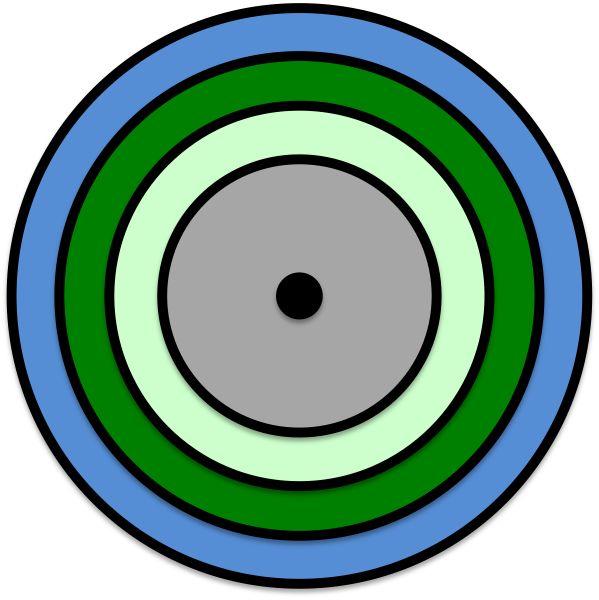
\includegraphics{Batches.png}
}
\end{center}
\caption{Pictorial representation of the integrand macrobatching scheme for the xc potential integration. 
Each of the colored regions represent a set of Lebedev spheres over several radial quadrature points, with the 
solid black dot representing the atomic nucleus. In the batching scheme, the scalar and matrix integrands
are evaluated over the entire batch simultaneously to improving caching and $\mu$-op behaviour.
}
\label{fig:Batching}       % Give a unique label
\end{figure}

\begin{figure}
\begin{center}
\resizebox{3.25in}{!}{%
  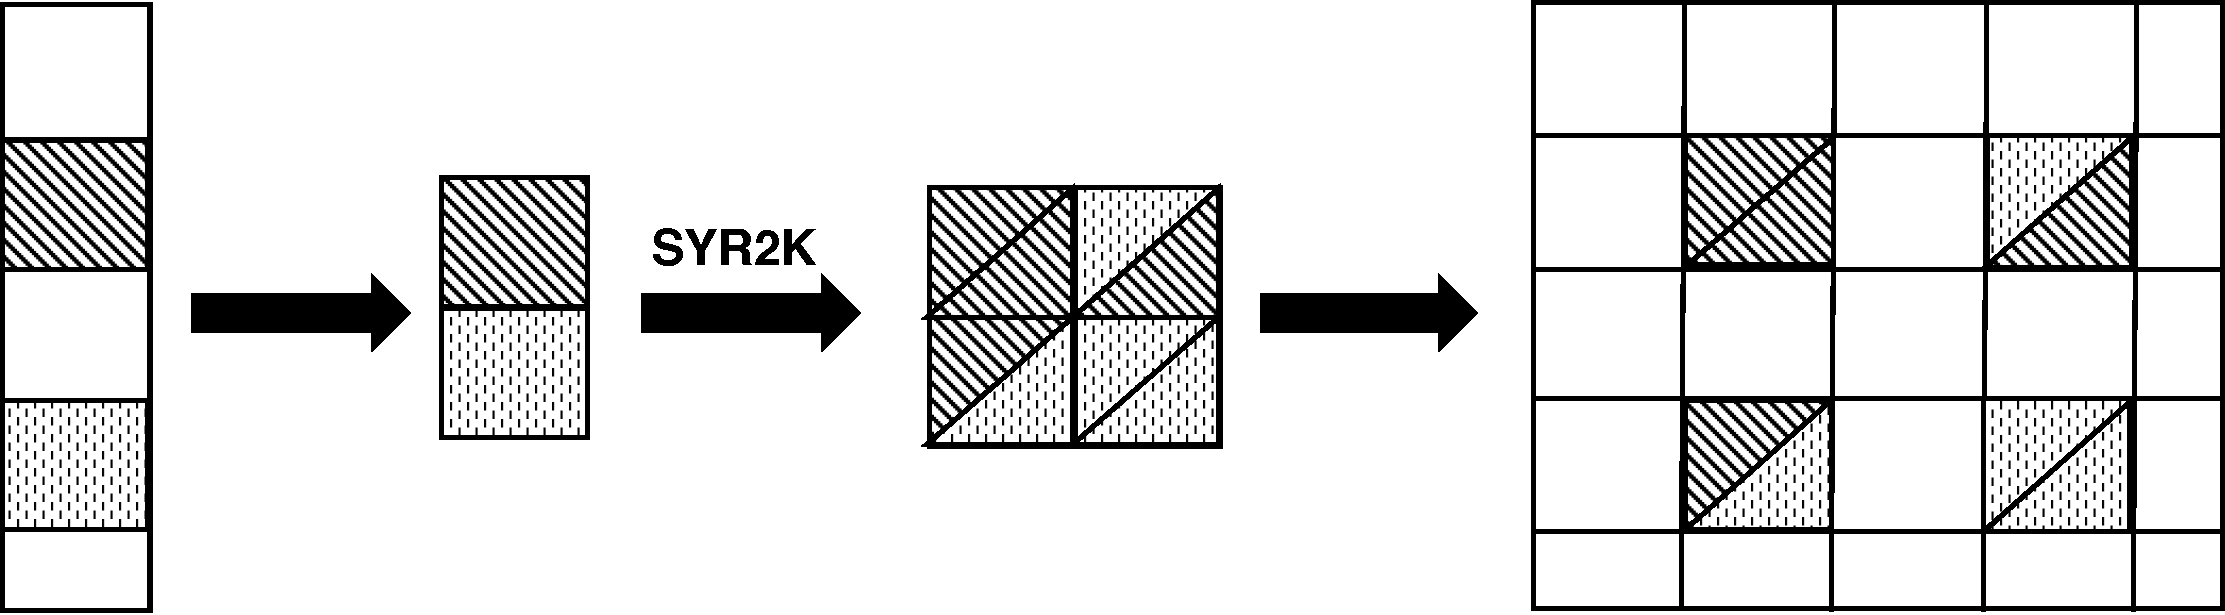
\includegraphics{Scheme2.pdf}
}
\end{center}
\caption{Pictorial representation of the screening and updating scheme for each
batch in the numerical integration of the xc potential.  A list of significant
basis functions in the batch (colored patterns in the figure) is selected and
than partitioned out for integration of that batch.  The accumulation of the
matrix integrand over the batch is evaluated by SYR2K  and then the final,
unscreened result is updated as shown. This scheme allows for only sequentional
memory access in the performance critical section of the integration and is
responsible for drastic performance increases.}
\label{fig:Integration}       % Give a unique label
\end{figure}

We may instead factor out a portion of the sum in \cref{eq:VXC_SYR2} such that
we may partition it into sum over batches of points.  In this work, we utilize a
macrobatch approach \cite{Frisch96_213}, where the grid points of each atoms are
grouped  into Lebedev spheres \cite{Lebedev77_99} of several radial quadrature points. This scheme
is pictorially represented in \cref{fig:Batching}. Denoting the set of all batches
as $\mathfrak B$, we obtain

\begin{align}
\label{eq:VXC_SYR2K}
\mathbf{V}^{GGA,I} &= \sum_{S_j \in \mathfrak B} \left(\sum_{i\in S_j} \mathbf{z}^I_i \boldsymbol{\chi}_i^T + \boldsymbol{\chi}_i \left(\mathbf{z}^I_i\right)^T \right) \nonumber \\
&= \sum_{S_j \in \mathfrak B} \mathbf{Z}^{I(j)} \left(\mathbf{X}^{(j)}\right)^T + \mathbf{X}^{(j)} \left(\mathbf{Z}^{I(j)}\right)^T
\end{align}
where
\begin{equation}
\mathbf{Y}^{(j)} = \begin{bmatrix} \mathbf{y}_1 & \mathbf{y}_{2} & \cdots & \mathbf{y}_i & \cdots &\mathbf{y}_{\vert S_j \vert} \end{bmatrix} \quad \forall i\in S_j,
\end{equation}
and $\mathbf{y}$ is either $\mathbf{z}$ or $\boldsymbol{\chi}$. \Cref{eq:VXC_SYR2K} is a sum over symmetric rank--2$k$ updates (SYR2K), where $k = \vert S_j \vert$. By tuning
$k$, one improves caching behavior dramatically. This is due to the fact that optimized implementations of SYR2K operations utilized efficient block
operations to optimize the flow of data to and from the computational caches. 
%  \todo{make a table / plot of cache misses + wall time for SYR2 and SYR2K}.}
 Similar schemes may
developed for the evaluation of the V variables (\cref{eq:VVarEval}) over batches using optimized matrix--matrix multiplication routines. However, while the caching behavior
is improved with increasing $k$, this is not the only consideration one needs take into account when partitioning the integration grid into batches.

The scheme in \cref{eq:VXC_SYR2K} may be further improved by recognizing the fact  that the basis functions typically used for molecular calculations carry 
a degree of spatial locality. 
A pictorial representation of the screening and updating scheme is given in \cref{fig:Integration}.
For each batch, we create a list of basis functions
that effectively overlaps it (colored subset of basis functions in \cref{fig:Integration}). 
This list of significant basis functions will be different for
each batch, but the number of basis
functions in each list becomes independent of size
for sufficiently large molecules, given the  spatial localization nature of Gaussian atomic centered basis sets.
%As such, not every basis function need be evaluated for every batch depending on the distance of the basis function to the points in the
%batch. Deciding which basis functions need to be evaluated are dependent on the characteristics of the basis set. \todo{explain / cite how we screen}. 
This reduced list of basis, evaluated for all points in the batch, is stored in contiguous blocks of memory, and used (along with the corresponding submatrices of the density-matrix, when required) for the evaluation of the potential, $\mathbf{Z}$ (see \cref{eq:ZKmu}), by exploiting a sub-sequential series of vectorized operations.
An important note here is that the maximum values for the batch of basis functions, $\chi_{max}(batch)$, and potential, $Z_{max}(batch)$, can be used to screen the entire contribution of the points in the batch to the integration. In this case, the integration can move to the next batch, avoiding the rank-2k update, that is the computationally most expensive part of the process,  without loosing accuracy.
Otherwise, recognizing that $\mathbf{Z}$ and $\mathbf{X}$ exhibit the same sparsity pattern, we may define
\begin{equation}
\tilde{\mathbf{V}}_{(j)}^{GGA,K} = \tilde{\mathbf{Z}}^{K(j)} \left(\tilde{\mathbf{X}}^{(j)}\right)^T + 
\tilde{\mathbf{X}}^{(j)} \left(\tilde{\mathbf{Z}}^{K(j)}\right)^T
\end{equation}
where moieties denoted with a tilde are the packed quantities where only the basis functions which have been chosen to be evaluated for the batch are represented.
The packed $\tilde{\mathbf{V}}_{(j)}^{GGA,K}$ may then be used to update the full $\mathbf{V}^{GGA,K}$ by mapping its elements to those in the full basis dimension.

\subsection{Discussion}

In this section, we will provide validation and computational performance
results for the proposed X2C-KS method. The proposed method was
implemented in a locally modified version of the open source
\texttt{ChronusQ} \cite{chronusq_beta2} electronic structure software package.
All calculations were performed using Intel Haswell compute nodes (14$\times$2
Intel\textregistered Xeon E5--2680 v4 CPUs @ 2.40 GHz, 32k L1 cache, 256k L2
cache, 35840k L3 cache) without the exploitation of molecular point group
symmetry. All numerical integrations were carried out with the Becke molecular
integration scheme using 100 Euler--Maclaurin~\cite{Laming93_997} quadrature points for the
radial integration and 302 Lebedev~\cite{Lebedev77_99} points for the angular integration around
each atom.

\subsubsection{Validation}
\label{sec:NCDFT_VALID}

A series of geometrically frustrated hydrogen rings were used to gauge the validity of the 
proposed X2C-KS implementation. Geometrically frustrated systems
provide an excellect test case for the validation of non--collinear electronic structure
methods as their lowest energy mean--field solutions break $\op{S}_z$ symmetry to minimize
Pauli repulsion \cite{Gross07_196405,Frisch07_125119,Frisch12_2193,Scuseria13_035117,Yamaguchi01_670,Blochl03_15772,Truhlar11_2629,Truhlar13_5349,Li15_154109} .
Unlike their collinear counter parts (such as RKS and UKS), X2C-KS (or more generally GKS)
is able to support this broken symmetry due to its explicit treatment of the full
spinor nature of the electronic density. To this end, a series of six Hydrogen rings ranging from 3 to
8 hydrogens were constructed such that each hydrogen was placed at 1 \AA~ spacing around 
an equidistant circle (see \cref{fig:rings}). Thus only the odd membered rings may be considered geometrically
frustrated. All calculations involving Hydrogen rings were performed using the X2C-B3LYP/6-311+G(D,P)
level of theory \cite{Becke93_5648,Parr88_785,Preuss89_200}. 
The scalar and spin densities of the Hydrogen rings solutions have been examined in \cref{fig:rings}. 


In comparison to the thorough discussion of geometric frustration of Hydrogren rings in Ref \cite{Li15_154109}, 
we can see that for the even numbered Hydrogren rings,
the symmetrical distribution of the spin and scalar densities indicates an anti--ferromagnetic spin
alignment; the same as one would get in a collinear solutions. This is further confirmed by the fact that
the expectation value of $\op{S}$ for these solutions was found to be zero, thus all spins must be antialligned.
While is this perhaps not the most
intetesting result in the context of non--collinear calculations, it does indicate that our implementation
collapses to the expected collinear behaviour if needed. Further, in the case that the spin density is small
in all space (the six membered Hydrogen ring), we can see that the the choice for the generalized auxillary
variables in \todo{reference eq} is a robust and accurate choice even in the worst case scenario.
The primary result of \cref{fig:rings} is that both the spin and scalar densities adopt a symmetrical
distribution even for the odd membered rings; a property which would be impossible in a collinear solution
due to the geometrical frustration of the system. An anti--ferromagnetic solution (the lowest energy
solution within the unrestricted formalism for the Slater determinant ground state) would yield an
asymmetric spin density \cite{Li15_154109}. Thus, our implementation of X2C-KS is able to reproduce the expected symmetries of
the non--collinear soltions for both even and odd membered Hydrogen rings, ensuring the robustness and 
reilability of the proposed method.





\begin{figure}
\begin{center}
\resizebox{6.5in}{!}{%
  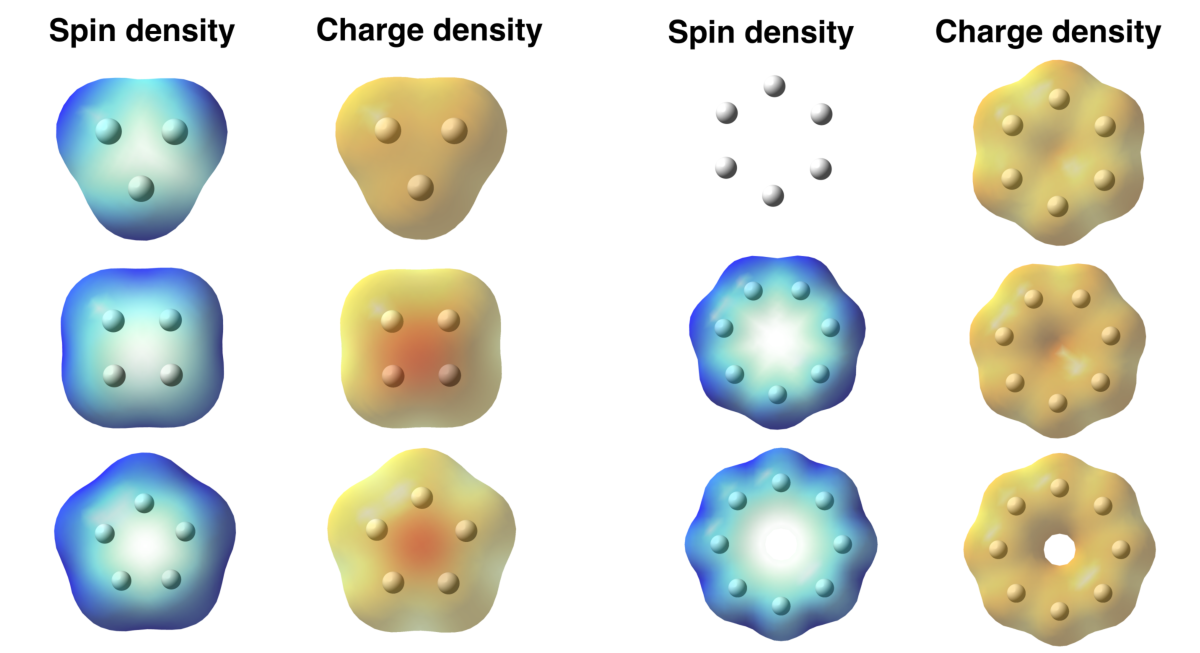
\includegraphics{rings.pdf}
}
\end{center}
\caption{X2C-B3LYP  6-311+g(D,P) spin ($\vert \vc{m}(\vc{r})\vert$, left) and scalar ($\rho^{1,0}(\vc{r})$, right) densities for a series of Hydrogen rings.
Blue and Red represent regions of greater density magnitude respectively.}
\label{fig:rings}       
\end{figure}

\subsubsection{Computational Performance}

\begin{figure}
\begin{center}
\resizebox{6.5in}{!}{%
  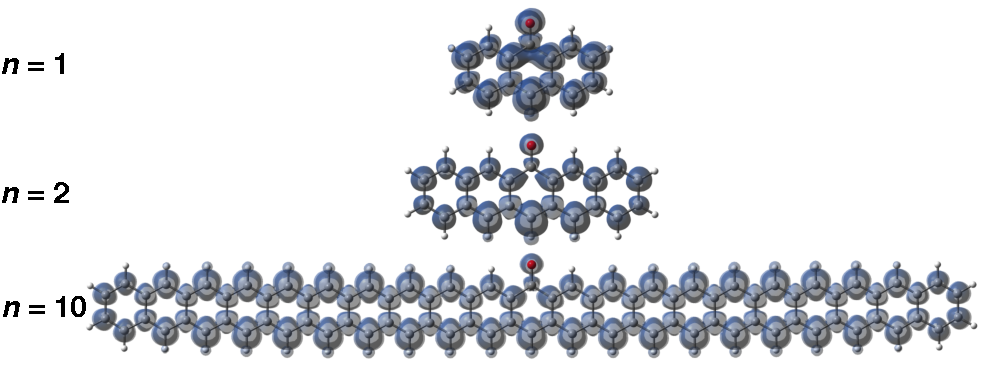
\includegraphics{radicals.pdf}
}
\end{center}
\caption{X2C-B3LYP 6-311+G(2D,P) spin densities ($\vert\vc{m}(\vc{r})\vert$) for phenoxy radicals with an increasing number of fused benzene rings 
($n$=1-10, where $n$ represents the number of fused benzene rings on each side).}
\label{fig:radicals}       
\end{figure}

In this section, we examine the computational performance of the proposed
X2C-KS method.  All the following tests presented were performed using
X2C-B3LYP/6-311+G(2D,P).  All times refer to the combined wall time for the
numerical evaluation of $ E^{GGA}$ and the matrix elements
$V^{GGA,K}_{\mu\nu}$ (\cref{eq:EXCGGA_num} and \cref{eq:VXCGGA_num}) as an
average over 5 SCF steps in the X2C-KS optimization.  

To demostrate the efficacy of our method relative to standard UKS methods,
we examine the relative scaling of UKS and X2C-KS with respect to system
size. For this numerical experiment we have choses a set of phenoxy radicals
shown in \cref{fig:radicals}. These systems were chosen as they exhibit highly
delocalized spin--density across their entire spatial extent. This allows for
a true comparison between UKS and X2C-KS as UKS will only support a particular
($z$) orientation of the magnetization vector while X2C-KS will not have this
restriction. Wall timings for single node (28 CPU core) performance on these systems are presented in \cref{fig:timing}.
As can be seen, the scaling of UKS and X2C-KS is identical with X2C-KS
having a slightly larger prefactor. In terms of raw wall timings, this increase in prefactor
does not ammount to a significant computational overhead over UKS. This is to be expected as there are (linearly)
more spin components of $\spvc V^{xc}$ is X2C-KS over UKS (per \cref{eq:DenFockConstraint}),
thus the only difference should amount to a prefactor.




To demostrate the scalability of the proposed method, we examine the parallel
performance of our implementation using the largest phenoxy radical from the
previous numerical experiment. Wall time as a function of the number of 
parallel processes utilized (1, 2, 4, 8, 12 nodes, for a total of 28, 56, 112, 224, 336 CPU cores)
for this system is are presented in \cref{fig:nodes}. The implementation of X2C-KS
is shown to exhibit linear scaling over parallel processors (a slope of -1.01).
As previously discussed in \cref{sec:NCDFT_IMPL}, this behaviour is expected
for a proper implementaion of any KS method as the operations which are to be performed
are completely independent. In out implementation, distributed memory parallelism
was achieved by placing each atomic integrand (per the Becke scheme) on
an individual MPI process while performing each atomic indegrand using shared
memory parallelism (OpenMP) of each node.

\begin{figure}
\begin{center}
\resizebox{3.25in}{!}{%
  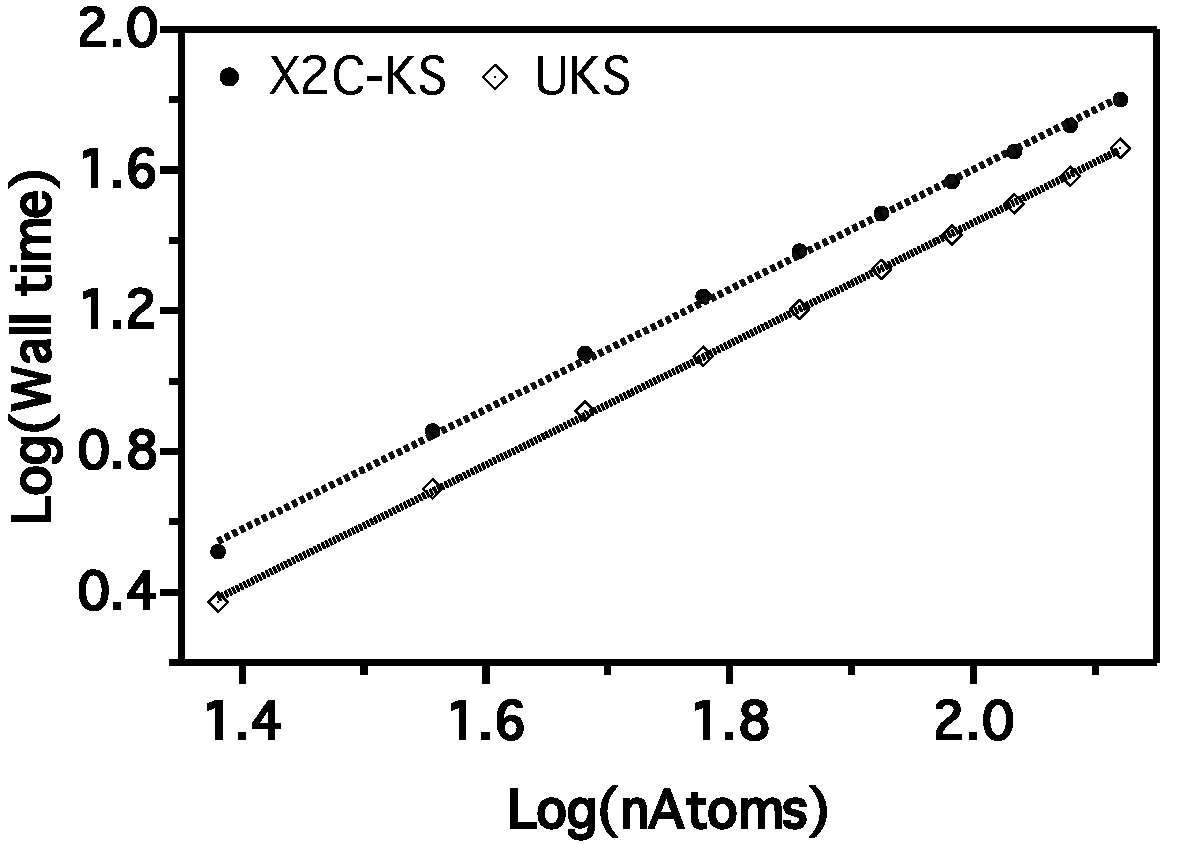
\includegraphics{timings_natoms.pdf}
}
\end{center}
\caption{
Relative scaling with respect to system size on a set of phenoxy radicals for
the UKS and proposed X2C-KS methods. Times are presented logarithmically to
demonstrate identical scaling with differing prefactors for the two methods.
Times presented are the average wall times for the numerical integration of
$E^{GGA}$ and $V_{\mu\nu}^{GGA,K}$ over 5 SCF steps.  
}
\label{fig:timing}     
\end{figure}

\begin{figure}
\begin{center}
\resizebox{3.25in}{!}{%
  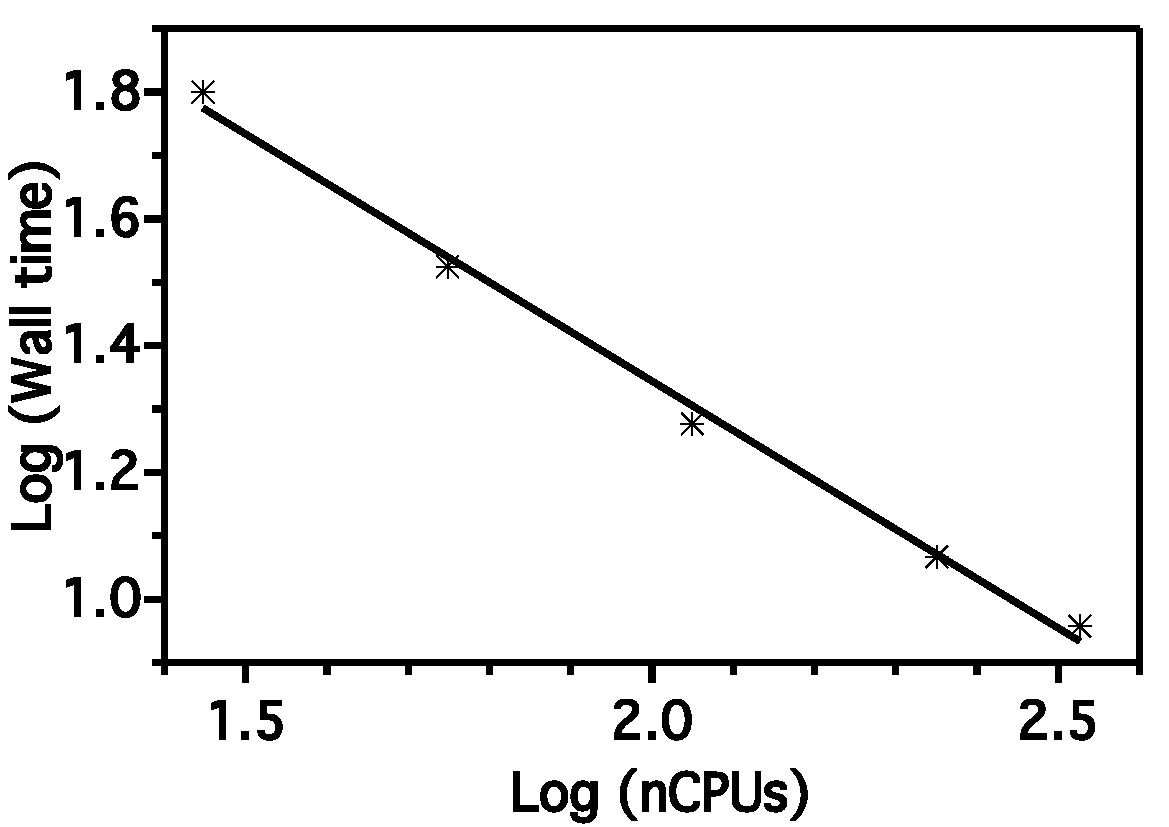
\includegraphics{cpus.pdf}
}
\end{center}
\caption{
Wall times for the distributed memory parallel performance of the proposed implementation of 
X2C-KS on a large phenoxy radical. Times are presented logarithmically to demonstrate the linear 
(-1.01) scaling of the proposed method.
Times presented are the average wall times for the numerical integration of
$E^{GGA}$ and $V_{\mu\nu}^{GGA,K}$ over 5 SCF steps.  
}
\label{fig:nodes}       
\end{figure}

\subsection{Conclusions}

In this work, we developed an efficient and scalable protocol for the
integration and assembly of the xc potential in non--collinear
KS-DFT. Initial numerical experiments demonstrate numerical stability
and robustness for the proposed method on a set of challengeing
molecular systems which exhibit non--collinearity due to geometrical
frustration. We have demonstrated excellent performance of
the proposed method both from the perspective of scaling with system
size and linear parallel scaling on distributed memory architechtures.
Further, we have shown that with the proposed algorithm, the computational 
cost relative to UKS is not significant. We hope that the proposed algorithm
will inspire development in relativistic DFT to move past proof of concept
and torwards leveraging the lastest advances in high--performance computing.




%In this work, we presented an integration and assembly strategy, 
%using a two-component spinor density, for efficient evaluation
%of the exchange correlation term using localized basis
%functions. 
%The presented formulation is suitable to exploit parallelism 
%along with optimal cache utilization and micro-architecture specific floating point operations.
%This leads to the evaluation of exchange correlation
%contributions with matrices of optimal sizes. 
%We also show that the proper choice of auxiliary variables 
%correctly give rise to nonzero local torque of the xc magnetic field on the magnetization
%while maintaining net zero global torque, as is expected from
%the exact functional. 
%Several tests were used to validate 
%the reliability and the performance of the proposed strategy.
%This approach can help to extend 
%the applicability of relativistic two-component DFT 
%to systems of large size ($>$ 100 atoms). 







\section{The Relativistic Particle--Particle Random Phase Approximation}

At times, the KS-DFT description is not sufficient for the proper description
of the electronic wave function. This case is encountered in general when
the wave function cannot be descibed properly as a single Slater determinant.
As such, in this section is oulined a two--component many--body expansion 
method (ala \cref{eq:ExcitationOp}) which includes relatativistic effects
and tackles the electron correlation problem though representing the wave function
as a linear combination of several Slater determinants. The following sections
have been adapted and reproduced with permission from David B. Williams--Young,
Franco Egidi, and Xiaosong Li. Relativistic Two--Component Particle--Particle
Tamm--Dancoff Approximation. \emph{J. Chem. Theory Comput.} \textbf{2016}, 12(11),
pp 5379-5384. Copyright 2016 American Chemical Society.




\subsection{Motivation}

The ability to accurately predict and characterize the electronically excited
states of molecular systems is paramount to a complete understanding of many
chemical phenomena. As such, excited states are the central focus of many
fields of physical chemistry, most prominent being that of spectroscopy. Due to
this centralized importance and the need to efficiently and accurately predict
excited states properties, much  effort has been devoted over the years towards
the modeling of excitation energies and oscillator strengths.


Recently, the particle-particle random phase approximation (pp-RPA) and 
Tamm-Dancoff approximation (pp-TDA), which have been standard trade tools of 
the nuclear physics community in the treatment of the many--body correlation energy for low matter density 
systems for some time \cite{SchuckBook_04}, 
have been extended to the treatment the correlation energy and excitation energies of quantum 
molecular systems within a finite basis set \cite{Yang13_224105,Yang13_18A522,
Yang13_174110,Yang13_104112,Yang13_030501,Yang09_066403,Bulik13_104113}.  Although the
introduction into the quantum chemistry community in relatively recent, a wealth 
of effort has been afforded to the rigorous investigation of these methods in a 
variety of different contexts, including the evaluation of excitation 
energies \cite{Yang13_224105,Yang13_18A522,Yang13_174110}, excited state properties 
and geometry optimizations \cite{Yang15_1025}, and the treatment of non-adiabatic 
phenomena such as non-adiabatic dynamics \cite{Liu14_244105} and the description 
of conical intersections \cite{Yang16_2407}.  So far in their development, however, 
these methods have only seen application in molecular systems using strictly 
collinear (RSCF and USCF) references, disallowing extension to systems with 
non--collinear (GSCF) reference, such as those that arise in spin-frustrated systems 
(see \cref{sec:NCDFT_VALID}) or whenever spin-orbit effects are included in the 
treatment of the electronic structure.


Recent years have also seen new developments in the realm of relativistic quantum 
chemistry.  Relativistic effects, while often neglected in most standard treatment
of electronic structure, can have profound consequences in chemical 
systems \cite{Pyykko12_45}.  Scalar relativistic effects cause the contraction of 
the core electron shells of heavy atoms, but perhaps of even more consequence is 
the introduction of spin couplings in the Hamiltonian.  Spin-spin and spin-orbit 
interactions can affect the electronic spin dynamics even in light atoms, and a 
direct consequence of these couplings on excited states is the loss of degeneracies
of spin-eigenstates, giving rise to fine structure splittings (FSS) in atoms and 
molecules with symmetry-induced degeneracies. It is therefore desirable to develop accurate and 
cost-effective relativistic electronic structure methods able to model such effects. 


Thus, in this work, we extend the pp-TDA formalism for use with 
relatvistic GSCF reference determinants, specifically the X2C-HF reference of \cref{sec:X2C,sec:MF2C}. 
However, the presented formalism may be employed in any case where the GSCF method must be
employed, such as the spin-frustrated systems explored in \cref{sec:NCDFT_VALID},
even in the absence of relativistic effects. 




\subsection{The Particle-Particle Tamm-Dancoff Approximation}
\label{subsec:ppTDA}
The pp-TDA is a non-particle-number conserving many--body expansion method, i.e. the
approximation of the excitation operator of \cref{eq:ExcitationOp} it employs does not commute with the number
operator.  To model a system with $N$ electrons, the pp-TDA starts from a
reference determinant for a system with $N-2$  electrons, and adds two
electrons back using an appropriate excitation operator.  The ground and
excited states of the $N$-particle system are thus obtained as ``excited
states'' of the $N-2$ electron reference, and the desired excitation energies
can be written as simple energy differences.  A general formalism for the
treatment of the pp-TDA within a finite basis of spin--collinear MOs has
described rigorously elsewhere
\cite{Yang13_224105,Yang13_18A522,Yang13_104112}.  Here, we review this
formalism for completeness and present the working expressions for the
relativistic X2C pp-TDA (X2C-pp-TDA) within the basis of MO spinors as well as
describe some caveats in the practical application of this method within the
context of a spinor reference.

From an (exact) $M$-particle ground state, $\ket{\Psi_0^M}$, the excitation operator
of \cref{eq:ExcitationOp} which constructs all ground and excited 
$N$-particle states ($\ket{\Psi_0^N}$ and $\ket{\Psi_n^N}$ respectively) may be written
convieniently as a projector $\op{R}^{N,M\dagger}_n = \ket{\Psi_n^N}\bra{\Psi_0^M}$, such that
\begin{equation}
  \ket{\Psi_n^N} = \op{R}^{N,M\dagger}_n \ket{\Psi_0^M}.
\end{equation}
Given such an ansatz, it is possible to construct an equation-of-motion (EOM) \cite{SchuckBook_04} 
for $\op{R}_n^{N,M\dagger}$, affording some corresponding
probing de-excitation operator $\delta \op{R}$ , to obtain the eigenenergies of $\ket{\Psi_n^N}$,
\begin{equation}
\label{eq:EOM}
  \left[ \delta \op{R},\left[ \op{H}, \op{R}_n^{N,M\dagger} \right]\right] = 
    (E^N_n - E^M_0)\left[\delta \op{R}, \op{R}^{N,M\dagger}_n \right].
\end{equation}

\Cref{eq:EOM} is formally exact and completely independent of the chosen
reference, provided one has access to the exact $N$- and $M$-particle states,
or eqivalently a closed form expression for the projector (such as \cref{eq:ExOpExp}).
In practice, one may take the expectation value of \cref{eq:EOM} using some
approximate $M$-particle ground state, which in the present work will be
a Slater determinant, $\ket{\Phi_0^M}$, to obtain
\emph{approximate} energy differences between $N$- and $M$-particle states
given some explicit (truncated) form of $\op{R}^{N,M\dagger}_n$.  As has been previously
discussed, if the $N$ and $M$ systems differ by exactly two particles ($M=N-
2$), the X2C-pp-TDA equation may be obtained by postulating that the excitation
operator take the form of all (unique) 2-particle additions to obtain
$N$-particle states from an $(N-2)$-particle reference,
\begin{equation}
  \op{R}_n^{N,(N-2)\dagger} = \sum_{a < b} X^n_{ab} \tau^{ab} , \label{eq:ppTDAExcitation}
\end{equation}
while the de-excitation operator takes the form
\begin{equation}
  \delta\op{R} = \tau_{ab}\quad.
\end{equation}
Here, $\tau$ is defined in \cref{eq:TauDef} and $X^n_{ab}$ is an expansion
coefficient that describes the contribution to the $n$-th $N$-particle state of
the addition of 2 particles into single-particle virtual states, $a$ and $b$,
of the $(N-2)$-particle ground state reference. By taking the expectation value
of \cref{eq:EOM} in a single X2C-HF Slater determinant (e.g. by using Wick's theorem) given
\cref{eq:ppTDAExcitation}, one obtains the Hermitian eigenvalue problem of the
X2C-pp-TDA
\begin{align}
\sum_{c < d} A_{ab,cd} X^n_{cd} &= \Omega_n X^n_{ab} \quad (a < b), \label{eq:ppTDA}\\
\Omega_n &= (E_n^N - E_0^{N-2}) \\
  A_{ab,cd} &= \delta_{ac}\delta_{bd} (\epsilon^\mathrm{X2C-HF}_a + \epsilon^\mathrm{X2C-HF}_b) + \innerop{ab}{r_{12}^{-1}}{cd} - \innerop{ab}{r_{12}^{-1}}{dc}  \quad \label{eq:AMat},
\end{align}
where  $\{\epsilon^\mathrm{X2C-HF}_p\}$ is the set of orbital
eigenenergies obtained from solving the X2C-HF equation in \cref{eq:X2CHFRH} and
\begin{equation}
  \innerop{ab}{r^{-1}_{12}}{cd} = \sum_{\mu\nu\lambda\kappa} \sum_{\sigma\sigma'} 
C^{\sigma*}_{\mu a}
C^{\sigma'*}_{\mu b}
C^{\sigma}_{\mu c}
C^{\sigma'}_{\mu d}
  \innerop{\mu\nu}{r^{-1}_{12}}{\lambda\kappa} \label{eq:ERI-MO}
\end{equation}
where $\innerop{\mu\nu}{r^{-1}_{12}}{\lambda\kappa}$ is defined in \cref{eq:ERIBasis} and $\spvc C = \spvc C^\mathrm{X2C-HF}$. 
One may obtain neutral $N$-particle excitations by examining the eigen spectrum of \cref{eq:ppTDA}. By
variationally optimizing the wave function of the $(N-2)$-particle system via
X2C-HF, both the $N$-particle ground and excited state energies are obtained
via
\begin{align}
E_n^N = E_0^{N-2} + \Omega_n \quad . \label{eq:ESEnergy}
\end{align}
Thus the excitation energy between $N$-particle ground and excited states, $\omega_n^N$, described via the X2C-pp-TDA may be written as differences of the eigenenergies,
\begin{equation}
\omega_n^N = E_n^N - E_0^N = \Omega_n - \Omega_0 \quad (n > 0). \label{eq:EXEnergy}
\end{equation}

These working expressions in \cref{eq:ppTDA,eq:AMat,eq:ESEnergy,eq:EXEnergy}
are similar to those previously expressed for the spin-collinear
reference \cite{Yang13_224105,Yang13_18A522,Yang13_104112}. The key difference
is that all of the above equations are expressed in a non--collinear GSCF spinor 
basis rather than a collinear (RSCF / USCF) orbital basis, and that the
orbitals have been optimized in the presence of relativistic spin-orbit
effects via the X2C method.
Unlike the collinear case, where significat simplification of \cref{eq:ppTDA} is
achieved through exploitation of the spin orthonality of the reference 
\cite{Yang13_224105,Yang13_174110}, the general non-collinear case presented in this
work cannot be further simplified.

\subsection{Results and Discussion}
\label{sec:ppX2CResults}

All calculations were performed with a locally modified version of the Gaussian
quantum chemistry suite of programs \cite{GDVI04}, and employed the
taug-cc-pVTZ-DK Gaussian basis set \cite{Dixon01_48} with the diffuse \emph{f}-functions
removed.  Relativistic effects were accounted for by means of the variational
X2C method outlined in \cref{sec:X2C,sec:MF2C}.
In order
to partially account for two-electron spin-orbit interaction in the
Hamiltonian, we employed a scheme based on the scaling of the nuclear charge
according to the angular momenta of the basis functions (\cref{eq:BScaling}). The atomic nuclei,
rather than being treated as point charges, were described using $s$-type
Gaussian charge distribution (\cref{eq:GauNuc}). The stability of the
two-component ground state wave function was also tested before X2C-pp-TDA
calculations were performed \cite{Li15_154109}.

\subsubsection{Single Excitations}
\label{subsec:SingleEx}
In order to highlight the capability of the pp-TDA method to describe excited
states within a relativistic framework, in this section we examine the FSS
of some atomic systems.  The presence of spin-orbit couplings 
lifts some of the energetic degeneracies that would be expected in the ground or
excited electronic states in non--relativistic theory.  
We therefore calculate the excitation energies of selected
atomic systems and compare the obtained fine structure splittings with
experimental reference values \cite{NIST_ASD} to asses the accuracy of the
method.  In this section we restrict ourselves to states describable by single
excitations (with respect to the $N$-electron system) which allows us to also
compare our results with the results obtained using the two-component
particle-hole Random-Phase Approximation (X2C-ph-RPA), also known as
Time-Dependent Hartree-Fock method (X2C-TDHF), as well as with results obtained
using the X2C-ph-TDA method \cite{Li16_3711}. Results for these FSS estimations 
are collected in \cref{tb:SingleEx}.

It can be seen that, in general, the three methods perform similarly with
respect to the reference values insofar as the order of magnitude of the error
is concerned. A general trend may be observed in that the X2C-pp-TDA
consistently overestimates the splittings as the atomic charge of the
underlying nucleus increases. This effect is magnified in the low energy
transitions while it is less apparent in the higher energy transitions. This is
due to the fact that the frontier orbitals of the ($N-2$)-reference being used
become sub-optimal in the proper description of the $N$-electron system due to
a contraction in the presence of higher nuclear charge. This leads to an
unphysically small energetic separation between the frontier orbitals of the
$N$-electron system which causes increasing errors due to an unphysical
increase in mixing. This problem is less obvious in higher energy excitation
because the higher lying orbitals are not as affected. These orbitals are
properly optimized in the X2C-ph-RPA/TDA due to orbital occupancy of the
resulting wave function. The general out-performance of the X2C-ph-TDA over the
X2C-ph-RPA may be attributed to an over estimation of electron correlation in
the ground and excited states via the RPA \cite{Dreuw05_4009}. The presence of
the de-excitation amplitudes in the X2C-ph-RPA allow for an over-mixing for the
low-lying excited states with the ground state which give rise to an
overestimate of the FSS, much the same as the case for the X2C-pp-TDA.
                                                                                                                                                 
 
                                                                                                                                                                                                                                                              
 
The main advantage of the particle-particle over the particle-hole formalism is
that, in the former, both the ground and electronically excited $N$-particle
states are described on equal footing with respect to correlation, being a
linear combination of several Slater determinants.  Conversely, in the ph-TDA
or ph-RPA method, the ground state is described as a single determinant, while
excited states are described as linear combinations of single excitations (and
possibly de-excitations).  That being said, the excitation space spanned by the
X2C-pp-TDA solutions does not include all chemically relevant excitations, many
of which can be found using the more traditional ph-RPA or ph-TDA methods.
This is due to the fact that the X2C-pp-TDA is, in its traditional form,
incapable of accessing excitations that involve contributions from below the
Fermi level.  Some work has been done in attempts to resolve this
problem \cite{Yang13_224105}, but these alterations to the pp-TDA method have
not been explored in this work.

\begin{table}[htbp]
  \caption{Calculated and reference \cite{NIST_ASD} excited-state fine structure splittings (in meV) for 
  single excitations of some atomic systems. The presence of a superscript ``$\circ$" in the term symbol 
  denotes an odd state with respect to space inversion.}
 \label{tb:SingleEx}
 \centering
 \begin{tabular}{llrrr}
  \hline
  Method     & Level                                              &  Mg   & Al$^+$ & Si$^{2+}$ \\ \hline
  X2C-ph-RPA & \multirow{3}{*}{$^3$P$^\circ_{1}-^3$P$^\circ_{0}$} &  4.89 & 10.49  & 19.85 \\
  X2C-ph-TDA &                                                    &  2.41 &  7.94  & 16.62 \\
  X2C-pp-TDA &                                                    &  2.77 &  9.13  & 18.97 \\
  Ref        &                                                    &  2.49 &  7.55  & 15.94 \\
  \hline
  X2C-ph-RPA & \multirow{3}{*}{$^3$P$^\circ_{2}-^3$P$^\circ_{1}$} &  9.75 & 21.02  & 39.96 \\
  X2C-ph-TDA &                                                    &  4.82 & 15.96  & 33.50 \\
  X2C-pp-TDA &                                                    &  5.55 & 18.40  & 38.40 \\
  Ref        &                                                    &  5.05 & 15.36  & 32.45 \\
  \hline
  X2C-ph-RPA & \multirow{3}{*}{$^3$P$^\circ_{1}-^3$P$^\circ_{0}$} &  0.33 &  1.82  &  4.43 \\
  X2C-ph-TDA &                                                    &  0.33 &  1.82  &  4.31 \\
  X2C-pp-TDA &                                                    &  0.42 &  2.17  &  5.08 \\
  Ref        &                                                    &  0.41 &  1.73  &  4.10 \\
  \hline
  X2C-ph-RPA & \multirow{3}{*}{$^3$P$^\circ_{2}-^3$P$^\circ_{1}$} &  0.67 &  3.67  &  9.09 \\
  X2C-ph-TDA &                                                    &  0.67 &  3.68  &  8.86 \\
  X2C-pp-TDA &                                                    &  0.84 &  4.50  & 11.04 \\
  Ref        &                                                    &  0.84 &  3.65  &  9.07 \\ 
  \hline
  \\
  \\
             &  &  MSE  &  MAE   & \\
  \hline
  X2C-ph-RPA &  &  2.32 &  2.28  & \\
  X2C-ph-TDA &  &  0.32 &  0.19  & \\
  X2C-pp-TDA &  &  1.55 &  1.55  & \\
  \hline
 \end{tabular}
\end{table}

\subsubsection{Triplet References and Double Excitations}
\label{subsec:DoubleEx}
In this section we wish to highlight other advantages of X2C-pp-TDA over
conventional X2C-ph-RPA.  In the previous section we presented results for
atomic systems that are characterized by being closed shell in both the $N$ and
$N-2$ systems.  This is important because if the reference state has unpaired
electrons then, as a consequence of the single reference nature of the
Hartree-Fock wave function, excited states will in general be
spin-contaminated, affecting one's ability to extract meaningful fine structure
splittings from the results, though adaptations to remedy this problem in the 
general case exist \cite{Liu10_064106,Suo11_134101,Liu11_194106,Liu12_024107,Liu13_3741}. By
using X2C-pp-TDA it is possible to treat systems with $N$ electrons
with any odd spin multiplicity, provided they become closed shell upon the
addition or removal of two electrons.  Molecules which possess triplet ground
states as well as diradical moieties may be taken as examples.  To demonstrate
this feature we compare the FSS of one set of excited states of molecular
oxygen with experimental data in \cref{tb:DoubleEx}.  The difference between
the calculated and measured value is just 2.5~meV, notwithstanding the
approximations intrinsic in our method (e.g.~the approximate treatment of
electron correlation and the two-electron spin-orbit contributions, or the
finite basis set).  Of course, the same reasoning can also be applied in
reverse: X2C-ph-RPA theory can be readily used to find excited-state FSS of
systems with a singlet ground state, however if the addition or removal of two
electrons produces an open-shell molecule, then X2C-pp-TDA will present some
spin-contamination in the computed excited-states.



One advantage that X2C-pp-TDA always has over X2C-ph-RPA theory, however, is
its ability to describe double excitations.  \Cref{tb:DoubleEx} compares
calculated and reference excited-state FSS of doubly-excited states of some
atomic moieties.  The performance of the method is similar as in the case of
single excitations presented in the previous section.  Such states cannot be
found among the excited states computed via X2C-ph-RPA.

\begin{table}[htbp]
 \caption{Excited-state fine structure splittings (in meV) for triplet
  and doubly excited electronic states calculated by the X2C-pp-TDA method.}
 \label{tb:DoubleEx}
 \centering
 \begin{tabular}{llrr}
  \hline
  System & Level & X2C-pp-TDA & Ref \cite{NIST_ASD,Krupenie72_423} \\ \hline
  O$_2$ & $^3\Delta_3-{^3\Delta_2}$ & 20.58 & 18.09 \\ \hline
  \multirow{2}{*}{Al$^+$} & $^3$P$_1-^3$P$_0$ & 9.20 & 7.75 \\ 
  & $^3$P$_2-^3$P$_1$ & 17.93 & 15.03 \\  \hline
  \multirow{2}{*}{Si$^{2+}$} & $^3$P$_1-^3$P$_0$ & 19.46 & 16.55 \\ 
  & $^3$P$_2-^3$P$_1$ & 37.88 & 32.06 \\    \hline
 \end{tabular}
\end{table}

%-------------------------------------------------------------------------------
% CONCLUSION
%-------------------------------------------------------------------------------
\subsection{Conclusion}

In this work, a scheme for the extension of the pp-TDA method to relativistic
two-component wave functions has been presented.  This scheme involves the
approximate decoupling of the large and small components of the relativistic
wave function by means of the X2C method, followed by an Hartree-Fock SCF
calculation on the system obtained by removing two electrons, in order to
obtain a set of complex spinor molecular orbitals.  The two-component reference
system is then used in the X2C-pp-TDA calculation that yields the ground and
excited states for the $N$-electron system.  The extension of the pp-TDA to a
two-component reference comes at the cost of the employing complex spinor
orbitals, and not being able to separate the problem into smaller sub-problems
as is done in the case of RHF or UHF references via spin integration.  The
increased computational cost highlights the ever pressing need for direct and
parallel implementations of post-SCF electronic structure methods, which is
exaggerated in the case of relativistic electronic structure calculations.

It has been shown that the X2C-pp-TDA method exhibits excellent results in the
prediction of the fine-structure splittings of the atomic and molecular species
considered here.  The results are comparable and at times better than those
obtained using X2C-ph-RPA \cite{Li16_3711}. In addition, the X2C-pp-TDA is able
to capture electronic excitations traditionally inaccessible by the
X2C-ph-RPA/TDA thanks to the 2-particle reference shift, such as double
excitations and those that would be described as spin-contaminated in
particle-number conserving methods.  While these results are promising, the
general applicability of the X2C-pp-TDA method, as with the spin-collinear
variant, is limited as it is traditionally unable to capture excitations that
involve contributions of orbitals from below the Fermi level.  That being said,
there are many systems, such as triplet and diradical systems, that the
X2C-pp-TDA provides a suitable method for the accurate description of the
electronic manifold.


\chapter{Molecular Response Properties Through Model Order Reduction}
\label{ch:MOR}


The previous sections have developed the formal theory to practically obtain the stationary 
(\cref{eq:TIQWave}) electronic ground and excited states of molecular systems.
While such developments provide the basis of any practical quantum theory, the majority of interesting chemical
phenomena result for the departure from the a stationary state through the action of some external perturbation,
i.e. light. In this chapter we will focus on the interaction and response of molecular systems with external 
electromagnetic fields which will allow us to probe many physically observable quantities such as
the photoabsorption cross section. The following sections have been adapted and reproduced in part with
permission from Roel van Beeumen, David B. Williams-Young, Joeseph M. Kasper, Chao Yang, Esmond G. Ng,
and Xiaosong Li. Model Order Reduction Algorithm for Estimating the Absorption Spectrum. 
\emph{J. Chem. Theory Comput.} \textbf{2017}, 13(10), pp 4950-4961. Copyright 2017 American Chemical
Society.


\section{Motivation}

With recent advances in  laser light source technology, X-ray
absorption spectroscopy (XAS) has become an important probative tool in
chemical physics.\cite{Stohr13_book} The ability of XAS to simultaneously
characterize both the electronic and geometrical structure of chemical systems
has made it indispensable in the fields of catalysis and
photophysics.\cite{Koch87_519,Chasse12_4870,Solomon95_2259,Hodgson00_5775,Hessler01_262}
However, despite the capability of XAS to obtain a wealth of chemically
relevant information, the complexity of experimentally obtained XAS spectra
often requires a theoretical supplement to obtain a meaningful interpretation
of the query phenomenon.\cite{Li16_639,Li16_JA2} Thus, the ability to properly
describe the high-energy electronic excitations of molecular systems
theoretically is critical in modern electronic structure theory.

In light of its importance in physical chemistry, the prediction of XAS properties poses an interesting challenge for traditional electronic structure methods. 
This challenge is rooted in the fact that the X-Ray region is buried deep within the eigenspectrum of the Hamiltonian and is often spectrally dense. 
For example, in near edge X-Ray absorption fine structure (NEXAFS) spectroscopy, the spectrum consists of many excited states that correspond to excitations of core electrons to diffuse quasi bound levels. 
Thus, as system sizes increase, the number of states in the given energy region increases dramatically. 
Further, it is important to note that, because very large basis sets are often required to properly describe the rather diffuse nature of these excited states, the increase in complexity leads to poor scaling with system size.

Many electronic structure methods have been extended to the
description of high-energy, X-ray electronic excitations in recent years. In
the time domain, real-time density functional theory\cite{Li05_233,Li07_199,Li11_184102} has been shown to
excellently reproduce the X-ray \emph{K}-edge for molecules within relatively
short simulation times.\cite{Govind12_3284,Lopata16_3741} For large systems,
however, time-domain methods have difficulty taking full advantage of
concurrency on modern computing architectures, and are thus not yet a
sustainable avenue in routine theoretical inquiry of these phenomena. In contrast,
frequency domain approaches are often favored in these types of calculations as
they may be cast as computationally scalable linear algebra problems which are
well suited for massive concurrency. Frequency domain approaches to treat
electronic excitations may be separated into two categories which obtain equivalent information:
methods which aim to obtain a spectral decomposition of the quantum propagator, i.e., eigenproblem based methods, and methods which solve the response problem directly through the solution of linear systems of equations. 

Recasting electronic structure methods into eigenproblems has long been the de facto standard frequency domain method for electronically excited states. Through knowledge of the poles (eigenroots) of the quantum propagator, one has direct access to information regarding the electronic excitations (resonances) of the molecular system. In addition, such a spectral decomposition may be used to treat off-resonant perturbations through interpolation schemes known as sum-over-states expressions\cite{Yeager84_33}.
Much work has gone into the development of these methods in both wave function theory, such as those based on
the 
coupled-cluster (CC)\cite{olje1988,Monkhorst77_421,Jorgensen90_3333,Bartlett93_7029,Bartlett93_414} 
and algebraic diagrammatic construction (ADC)\cite{Dreuw14_4583,Dreuw14_1900} 
expansions of the many-body wave function,
and self-consistent field theory, such as the linear response time-dependent Hartree--Fock (TD-HF)\cite{Hattig98_1,Ring_book,Jorgensen_book,Rowe68_153} and density functional theory
(TD-DFT)\cite{Casida95_book,HeadGordon05_4009}. These methods have been shown to accurately predict and reproduce both low-\cite{Ruud12_543,Bartlett09_Book} and high-energy\cite{Li11_3540,Li15_2994,Li15_4146,DeSimone03_115,Neese07_2783,Asmuruf10_12024,Govind12_3284} electronic excitations in molecular systems.  Despite
their accuracy, however, eigenproblem based methods possess an inherent challenge in the
description of high-energy excited states when the eigenroots of interest
are buried deep in the eigenspectrum.  Traditional methods used to partially
diagonalize the propagator, such as the
block-Davidson method\cite{Davidson75_87,Scott86_817,Morgan92_287}, are designed to converge to the extreme ends of the
eigenspectrum with no built-in mechanism to establish the spectrum's interior. 
Several approaches have been described to overcome this problem~\cite{zuev_etal2015}, including
energy specific\cite{Li11_3540,Li15_4146} and
restricted energy window methods\cite{DeSimone03_115,Neese07_2783,Asmuruf10_12024} when the eigenroots of interest are well-separated. Further, in spectrally dense regions of the propagator's eigenspectrum, iterative diagonalization algorithms require the resolution of many more roots than is often practical to ensure smooth convergence.

Methods which solve the response problem through the solutions of linear systems offer an attractive alternative to eigenproblem based approaches in the description of high-energy excitations because they have an intrinsic
mechanism to probe the interior of the energy spectrum. In these methods, the
probing frequency of the applied perturbation is a chosen parameter.\cite{Hattig98_1,Ruud12_543} Thus,
the interior of the spectrum is easily probed through a number of solutions
of linear system of equations in the desired frequency domain. This simplicity 
does, however, come at a seemly significant computational cost compared to eigenproblem based methods.
While eigenproblems are able to directly obtain many poles of the eigenspectrum
simultaneously, one must solve the linear problem many times
over some discretization of the frequency domain to obtain similar results.
In general, this discretization must be quite dense to achieve a reasonable 
accuracy and thus can be more expensive than their eigenproblem based counterparts. Approaches using linear systems and based on the complex
polarization propagator (CPP), such as CPP-CC\cite{Norman12_1616,Norman13_124311,Coriani13_211102} and CPP-SCF,\cite{Rubio_Book,Ruud12_543,Yeager84_33,Oddershede01_JCP}
have been shown to be successful in the description of both high\cite{Norman16_1991,Norman12_022507,Norman10_5096,Agren06_143001,Norman16_13591} and low\cite{Mathieu15_21866} energy properties of molecular systems and have been extended to relativistic Hamiltonians as well\cite{Norman10_064105}.

In this work, we introduce a general framework for the prediction of spectrally interior molecular response properties based on model order reduction (MOR) via interpolation. MOR techniques have been successfully applied in different fields of computation science and engineering, where it reduces the computational complexity of mathematical models in numerical simulations. Examples include structural dynamics, sound and vibration analysis, and control theory \cite{Antoulas2005}. The MOR algorithm proposed in this paper aims to overcome the large computational overhead associated with the spectral discretization required by linear system based methods while maintaining the accuracy associated with eigenproblem based methods. Further, the proposed algorithm will be shown to allow for the massively scalable parallelism that is well suited for modern computing architectures.

% ============================================= %
% == LINEAR RESPONSE AND ABSORPTION SPECTRUM == %
% ============================================= %
\section{Linear response and absorption spectrum}
\label{sec:lras}

In the semi-classical theory of molecular light-matter interaction within the electric dipole approximation, the isotropic absorption cross section for the interaction with plane-polarized light, $\sigma(\omega)$, at a particular perturbing frequency, $\omega$, is proportional to the trace of the dynamic polarizability tensor, $\bfalpha(\omega)$,
\begin{equation}
  \sigma(\omega) \propto \omega \imag\left(\trace\left[ \bfalpha(\omegat) \right]\right), \qquad \omegat = \omega + i\eta,
  \label{eq:abs-spectrum}
\end{equation}
where $\eta > 0$ is a small damping parameter to ensure the convergence of $\bfalpha$ in the spectral neighborhoods of resonant perturbations. Within the linear response regime of the first-order polarization propagator approximation (FOPPA)\cite{Yeager84_33}, the dynamic polarizability tensor may be written as
\begin{equation}
  \bfalpha(\omegat) = \bfd\T \bG\inv(\omegat) \bfd, \qquad 
  \bfd = \begin{bmatrix}
    \bfd_x & \bfd_y & \bfd_z \\
    \bfd_x & \bfd_y & \bfd_z
  \end{bmatrix}.
  \label{eq:polar-tensor}
\end{equation}
Here, $\{ \bfd_\xi\text{ } \vert\text{ } \xi \in \{ x,y,z \} \}$ is the set of
dipole operators expressed in the MO basis.
In the following algorithmic developments, we restrict the discussion to the FOPPA using a
Hartree--Fock reference (TD-HF), although the algorithm presented is completely
general to any choice of propagator or reference. Within TD-HF, $\bG(\omegat)$
may be written as
\begin{equation}
  \bG(\omegat) = \bH - \omegat\bS,
  \label{eq:defG}
\end{equation}
where
\begin{equation}
  \bH = \begin{bmatrix}
    \bA & \bB \\
    \bB & \bA
  \end{bmatrix}, \qquad
  \bS = \begin{bmatrix*}
    \bI & \vc 0 \\
    \vc 0 & -\bI
  \end{bmatrix*},
  \label{eq:defH}
\end{equation}
with $\bS = \bS\T = \bS\inv$ and
\begin{subequations}
  \label{eq:FOPPA-defs}
\begin{align}
  &A_{ai,bj} = \innerop{0^\HF}{[\tau^i_a,[\op H^\BO_{el}, \tau_j^b]]}{0^\HF} = 
    \delta_{ij}\delta_{ab}(\epsilon^\HF_a - \epsilon^\HF_i) + \innerop{aj}{r_{12}^{-1}}{ib} - \innerop{aj}{r_{12}^{-1}}{bi} \\
  &B_{ai,bj} = \innerop{0^\HF}{[\tau^a_i,[\op H^\BO_{el}, \tau_j^b]]}{0^\HF} = 
    \innerop{ab}{r_{12}^{-1}}{ij} - \innerop{ab}{r_{12}^{-1}}{ji} \\
  &d_{\xi,ai} = \innerop{0^\HF}{[\op O^1,\tau^{a}_i]}{0^\HF} = \innerop{\phi_a}{\op r_\xi }{\phi_i}
\end{align}
\end{subequations}
Here, we have denoted $\ket{0^\HF}$ as the HF ground state and $\{\op r_\xi\}$ as to components of the position
operator. $\{\epsilon^\HF_p\}$ is obtained by solving \cref{eq:RHEq} and the integrals $\innerop{\cdot}{r^{-1}_{12}}{\cdot}$
are given as in \cref{eq:ERI-MO}. Further, we have adopted the index convention for occupied and unoccupied HF-MOs
as in \cref{sec:SQ}. The definitions in \cref{eq:FOPPA-defs} are general to both two-component relativistic and 
non-relativistic HF references. However, in the following, we will restrict our treatment to that of non-relativistic theory
such that we may emply the use of strictly real HF-MOs. This will allow for signification simpliciation of the resulting
expressions.


In order to study the spectrum of the pencil $(\bH,\bS)$ let
\begin{equation}
  \bOmega = \bS\inv\bH = \begin{bmatrix*}
    \bA & \bB \\
    -\bB & -\bA
  \end{bmatrix*}.
  \label{eq:defOmega}
\end{equation}
Although the matrix $\bOmega$ is non-symmetric, it has a number of special properties \cite{olje1988,beme1998,bali2012}. 
If $\bH$ is positive definite, it may be shown that $\bOmega$ possesses a structured eigendecomposition \cite{Jorgensen_book,SJYDL2016}, i.e.,
\begin{equation}
  \begin{bmatrix*} \bA & \bB \\ -\bB & -\bA \end{bmatrix*}
  = \begin{bmatrix*} \bU & \bV \\ \bV & \bU \end{bmatrix*}
    \begin{bmatrix*} \bLambda & \vc 0 \\ \vc 0 & -\bLambda \end{bmatrix*}
    \begin{bmatrix*} \bU & -\bV \\ -\bV & \bU \end{bmatrix*}\T
\end{equation}
where $\bLambda = \diag(\lambda_1,\dotsc,\lambda_n)$ consists of strictly positive eigenvalues, 
and the eigenvectors are normalized with respect to the metric $\bS$,
\begin{equation}
  \begin{bmatrix*} \bU & -\bV \\ -\bV & \bU \end{bmatrix*}\T
  \begin{bmatrix*} \bU &  \bV \\  \bV & \bU \end{bmatrix*} = \bI.
  \label{eq:eigvec-normalization}
\end{equation}

As $\bH$ is taken to be real in this work, it possesses additional properties that may be exploited in the development of efficient algorithms for estimating the absorption spectrum of the target system. In particular, we may apply the following similarity transformation
\begin{equation}
  \bT = \frac{1}{\sqrt{2}} \begin{bmatrix*}
     \bI & \bI \\
    -\bI & \bI
  \end{bmatrix*}, \qquad \bT\inv = \bT\T,
\label{eq:defT}
\end{equation}
to $\bG(\omegat)$, yielding
\begin{equation}
  \bT\T \bG(\omegat) \bT = \begin{bmatrix}
    \bK & \vc 0 \\
    \vc 0 & \bM
  \end{bmatrix} - \omegat \begin{bmatrix}
    \vc 0 & \bI \\
    \bI & \vc 0
  \end{bmatrix},
  \label{eq:}
\end{equation}
where
\begin{align}
  \bM &\equiv \bA + \bB, \label{eq:defM} \\
  \bK &\equiv \bA - \bB, \label{eq:defK}
\end{align}
which are, in most cases, positive definite. In this case, the polarizability tensor may be reformulated as
\begin{equation}
  \bfalpha(\omegat) = \bfdt\T \bGt\inv(\omegat) \bfdt, \qquad \bfdt = \begin{bmatrix}
    \bfd_x & \bfd_y & \bfd_z
  \end{bmatrix},
  \label{eq:polar-tensor-MK}
\end{equation}
where
\begin{equation}
  \bGt(\omegat) = \bM\bK - \omegat^2\bI.
  \label{eq:defGt}
\end{equation}
Note that the dimension of $\bGt(\omegat)$ is only half the dimension of $\bG(\omegat)$. Furthermore, it can be shown that
\begin{align}
 \bM &= (\bX - \bY) \bLambda (\bX - \bY)\T, \\
 \bK &= (\bX + \bY) \bLambda (\bX + \bY)\T,
\end{align}
and
\begin{equation}
  (\bX - \bY)\T (\bX + \bY) = \bI,
\end{equation}
such that the eigenvalues $\pm\bLambda$ may be computed by
\begin{equation}
  \bM\bK = (\bX - \bY) \bLambda^2 (\bX + \bY)\T.
\end{equation}
Remark that by making use of $\bM\bK$, the dimension of the eigenvalue problem is also reduced by a factor of 2.\cite{Haser93_1262,Frisch98_8218}


\section{Interpolatory Model Order Reduction of Linear Dynamical Systems}
\label{lds:dyn-sys}

In this section, we briefly review the theory of model order reduction for
linear dynamical systems. The next section will examine its connection to the
computation of the absorption spectrum within the FOPPA.

% --- Linear dynamical systems --- %
\subsection{Linear dynamical systems}
\label{lds:mimo}

We consider the linear multiple-input multiple-output (MIMO) system
\begin{equation}
  \bSigma = \left\{\begin{aligned}
    \left( \bH - s\bS \right) \bfx(s) &= \bfb\,u(s) \\
                              \bfy(s) &= \bfc\T \bfx(s)
  \end{aligned}\right.,
  \label{eq:siso}
\end{equation}
where $s$ is a derivative or shift operator, $\bH \inRR{n}$ and $\bS \inRR{n}$ are the system matrices, $\bfb \inR[n][m]$, and $\bfc \inR[n][p]$. We call $n$ the dimension  (order) of the system $\bSigma$, $\bfx \inR[n][m]$ the state vector, $u \inR$ the input, and $\bfy \inR[p][m]$ the output \cite{Antoulas2005}. Note that the system $\bSigma$ is completely characterized by the quadruple $(\bH,\bS,\bfb,\bfc)$.

The transfer function, $\bfvarpi(s)$, of $\bSigma$ is defined as
\begin{equation}
  \bfvarpi(s) = \bfc\T \left( \bH - s\bS \right)\inv \bfb,
  \label{eq:siso-tf}
\end{equation}
and describes the relation between the input and output of $\bSigma$, i.e., $\bfy(s) = \bfvarpi(s) u(s)$. For the remainder, we will assume that $n \gg 1$, $m \ll n$, $p \ll n$, and $u(s) \equiv 1$ for all $s$.

% --- State space transformation --- %
\subsection{State space transformation}
\label{lds:ss-transf}

In some cases, it might be more advantageous to describe the system from a different point of view as the original one. In these cases, we may perform a non-singular state transformation $\bT$, i.e., $\det(\bT) \neq 0$, yielding the transformed state
\begin{equation}
  \bfxt = \bT\inv \bfx,
  \label{eq:defxtil}
\end{equation}
of the transformed system
\begin{equation}
  \bSigmat = \left\{\begin{aligned}
    \left( \bHt - s\bSt \right) \bfxt(s) &= \bfbt\,u(s) \\
                                 \bfy(s) &= \bfct\T \bfxt(s)
  \end{aligned}\right.,
\end{equation}
where $\bHt = \bT\inv \bH \bT$, $\bSt = \bT\inv \bS \bT$, $\bfbt = \bT\inv \bfb$, and $\bfct\T = \bfc\T \bT$. Remark that $\bSigma$ and $\bSigmat$ admit the same transfer function as well as the same output. Therefore, we call the systems $\bSigma$ and $\bSigmat$ equivalent.

% --- Reduced order models --- %
\subsection{Reduced order models}
\label{lds:mor}

The evaluation of the transfer function of a system $\bSigma$ requires a linear system solve for every value of $s$. In cases where the system dimension $n$ is large and a high resolution is required, i.e., a high number of values of $s$, the evaluation of the transfer function is very expensive. In this work, we examine the effectiveness of model order reduction (MOR) techniques to circumvent this expense. MOR for linear dynamical systems is a technique that approximates a system $\bSigma$ by another system $\bSigmah$ of the same form but of a much lower dimension (order) $k \ll n$. Consequently, evaluating the transfer function of $\bSigmah$ is relatively inexpensive as it only involves linear system solves of dimension $k$ instead of linear system solves of dimension $n$ for $\bSigma$.

Let the system $\bSigma$ be given by \eqref{eq:siso} and define a non-singular matrix $\bV \inR[n][k]$ with orthonormal columns, i.e., $\bV\T \bV = \bI$. Then, a reduced order model $\bSigmah$ can be constructed by applying a Galerkin projection $\bP = \bV\bV\T$ onto $\bSigma$, yielding
\begin{equation}
  \bSigmah = \left\{\begin{aligned}
    \left( \bHh - s\bSh \right) \bfxh(s) &= \bfbh\,u(s) \\
                                \bfyh(s) &= \bfch\T \bfxh(s)
  \end{aligned}\right.,
\end{equation}
where $\bHh = \bV\T \bH \bV$, $\bSh = \bV\T \bS \bV$, $\bfbh = \bV\T \bfb$, and $\bfch\T = \bfc\T \bV$. Note that the length of the state vector $\bfxh$ and the dimension of $\bSigmah$ are only $k \ll n$. The purpose of MOR is to construct a $\bV$ such that the transfer function of $\bSigmah$ approximates very well the one of $\bSigma$,
\begin{equation}
  \bfvarpi_\bSigma(s) \approx \bfvarpi_{\bSigmah}(s),
  \label{eq:tf-match}
\end{equation}
for all query $s$.

% --- Model order reduction via moment matching --- %
\subsection{Model order reduction via moment matching}
\label{lds:mm}

One way to construct a matrix $\bV$ such that \eqref{eq:tf-match} holds is by examining the concepts of moments and moment matching\cite{Antoulas2005}. Let the transfer function $\bfvarpi$ of $\bSigma$ be given by \eqref{eq:siso-tf}. Then the $\ell$th moment of $\bfvarpi$ around the point $s = s_\star$ is defined as the $\ell$th derivative of $\bfvarpi$ evaluated at $s_\star$, i.e.,
\begin{equation}
  \bfm_\ell(s_\star) := (-1)^\ell \left.\frac{d^\ell}{ds^\ell} \bfvarpi(s) \right|_{s=s_\star},
  \label{eq:moment}
\end{equation}
for $\ell \geq 0$. Consequently, since $\bfvarpi(s) = \bfc\T \left( \bH - s\bS \right)\inv \bfb$, the moments at $s_\star$ are
$$
  \bfm_\ell(s_\star) = \bfc\T \left( \bH - s_\star \bS \right)^{-(\ell+1)} \bfb, \qquad \ell > 0.
$$
Note also that the moments determine the coefficients of the Taylor series expansion of the transfer function $\bfvarpi$ in the neighborhood of $s_\star$
\begin{equation}
  \bfvarpi(s) = \bfm_0(s_\star) + \bfm_1(s_\star) \frac{s - s_\star}{1!} + \bfm_2(s_\star) \frac{(s - s_\star)^2}{2!} + \cdots
\end{equation}

Model order reduction via moment matching consists of constructing a subspace $\bV \inR[n][km]$ such that the original and reduced order model match moments
\begin{equation}
  \bfm_{i_j}(s_j) = \bfmh_{i_j}(s_j), \qquad j = 1,\ldots,k.
  \label{eq:mor-mm}
\end{equation}
If all moments to be matched are chosen at zero, i.e., $s_j = 0$ for $j = 1,2,\ldots,k$, the corresponding model is known as a Pad\'{e} approximation. In the general case, the problem \eqref{eq:mor-mm} is known as rational interpolation and can be solved by choosing the projection matrix $\bV$ such that
\begin{equation}
  \bV = \Span { \left( \bH - s_1\bS \right)\inv \bfb \quad
                   \left( \bH - s_2\bS \right)\inv \bfb \quad
                    \cdots \quad
                   \left( \bH - s_k\bS \right)\inv \bfb }.
  \label{eq:defV-app}
\end{equation}
It can be shown that the matrix $\bV$ defined in \eqref{eq:defV-app} spans a rational Krylov subspace and matches all the $0$th moments at $s_j$. For more information about the connections between moment matching and rational interpolation, we refer the interested reader to Section~11 of Antoulas' model order reduction book \cite{Antoulas2005}.

\section{Estimating absorption spectrum without explicitly computing eigenvalues and eigenvectors}
\label{sec:est}

The most straightforward way to evaluate the absorption spectrum is to compute eigenvalues and the corresponding eigenvectors of $(\bH,\bS)$. However, as we indicated earlier, when the dimension of $\bH$ and $\bS$ becomes large (spectrally dense), this approach can be prohibitively expensive (complicated). 

It has been shown\cite{brabec_etal2015} that a special $\bK$-inner product
Lanczos algorithm can be used to provide a good approximation to the overall
structure of the absorption spectrum without explicitly computing the
eigenvalues and eigenvectors of $(\bH,\bS)$.  In particular, the Lanczos
algorithm can reveal major absorption peaks in the low frequency region of the
spectrum without too many iterations. However, the algorithm gives limited
resolution of the absorption spectrum in the spectral interior as the
Krylov subspace constructed by the Lanczos iteration contains little spectral
information associated with interior eigenvalues of $(\bH,\bS)$.

We now propose an alternative way to evaluate the absorption spectrum without explicitly computing the eigenvalues and eigenvectors of $(\bH,\bS)$. This scheme focuses on approximating the dynamic polarizability tensor $\bfalpha(\omegat)$ defined in \eqref{eq:polar-tensor} and the absorption spectrum $\sigma(\omega)$ defined in \eqref{eq:abs-spectrum} within a specific energy window directly.

Firstly, observe that the dynamic polarizability tensor \eqref{eq:polar-tensor} may be viewed simply as the expectation value of the inverse of $\bH -\omegat \bS$. Hence, the evaluation of $\bfalpha(\omegat)$ may be recast into a problem of solving linear equations, i.e., for a specific frequency $\omega$, we can directly evaluate the absorption spectrum \eqref{eq:abs-spectrum} as follows
\begin{equation}
  \sigma(\omega) \propto \omega \imag\left(\trace\left[ \bfd\T \bfx(\omegat) \right]\right),
\end{equation}
where $\bfx$ is the solution of the linear system
\begin{equation}
  \left( \bH - \omegat\bS \right) \bfx(\omegat) = \bfd.
  \label{eq:lin-sys}
\end{equation}

Secondly, the dynamic polarizability tensor \eqref{eq:polar-tensor} may also be viewed as the transfer function, i.e., the relation between input and output, of the linear dynamical system (see \cref{lds:mimo})
\begin{equation}
  \left\{\begin{aligned}
    \left( \bH - \omegat\bS \right) \bfx(\omegat) &= \bfd \\
                                     \bfy(\omega) &= \bfd\T \bfx(\omegat)
  \end{aligned}\right..
  \label{eq:MIMO}
\end{equation}
Consequently, the absorption spectrum can directly be obtained from the output variable $\bfy$
\begin{equation}
  \sigma(\omega) \propto \omega \imag\left(\trace\left[ \bfy(\omega) \right]\right).
\end{equation}
In order to evaluate the output $\bfy$ of system \eqref{eq:MIMO} for a given frequency, we again need to solve a linear system of the form \eqref{eq:lin-sys}.

Finally, by exploiting the block structure of $\bH$ and performing a state space transformation with \eqref{eq:defT} (see \cref{lds:ss-transf}), we obtain an equivalent linear dynamical system for \eqref{eq:MIMO}, but with a halved order,
\begin{equation}
  \left\{\begin{aligned}
    \left( \bM\bK - \omegat^2\bI \right) \bfxt(\omegat) &= \bfdt \\
                                           \bfy(\omega) &= 2\,\bfdt\T \bK\,\bfxt(\omegat)
  \end{aligned}\right.,
  \label{eq:MIMO-MK}
\end{equation}
such that we obtain the following, compact expressions for the dynamic polarizability tensor
\begin{equation}
  \bfalpha(\omegat) = 2\,\bfdt\T \bK \left( \bM\bK - \omegat^2\bI \right)\inv \bfdt,
  \label{eq:polar-tensor-lin-MK}
\end{equation}
and the absorption spectrum
\begin{equation}
  \sigma(\omega) \propto \omega \imag\left(\trace\left[ \bfdt\T \bK \left( \bM\bK - \omegat^2\bI \right)\inv \bfdt \right]\right).
  \label{eq:abs-spectrum-lin-MK}
\end{equation}
Note that the dimension of the linear systems to be solved in \eqref{eq:abs-spectrum-lin-MK} is only half of the dimension of the linear system shown in \eqref{eq:lin-sys}.

Clearly, we cannot afford to evaluate $\sigma(\omega)$ for all $\omega$'s of interest. However, this connection to linear dynamical systems allows us to employ MOR techniques (see \cref{lds:mor}) to reduce the number of $\sigma(\omega)$ evaluations in the full dimension. More precisely, we construct a function $\hat{\sigma}(\omega)$ that approximates $\sigma(\omega)$ within a specific energy window $[\omega_\mathrm{min},\omega_\mathrm{max}]$, but is much cheaper to evaluate.  The construction of such an approximate function only requires solving a few linear systems of the form \eqref{eq:lin-sys} or \eqref{eq:MIMO-MK} at a few selected frequencies $\tau_j$, $j = 1,2,\ldots,k$. The solutions of these linear systems are then used to construct a reduced order model which interpolates the full dynamic polarizability at $\tau_j$, and provides an approximation to the dynamic polarizability tensor \eqref{eq:polar-tensor} at other frequencies within the predefined energy window. When $k$ is small, both the construction and the evaluation of the reduced order model is significantly lower than other approaches that are either based on solving an eigenvalue problem or \eqref{eq:lin-sys} at many different frequencies.

% ==================================== %
% == INTERPOLATION BASED ALGORITHMS == %
% ==================================== %
\section{Interpolation based algorithms}
\label{sec:mor}

Let the dimension of the matrix $\bH$ defined in \eqref{eq:defH} be $2n \times 2n$. The dimension of the lower dimensional matrix $\bHh$ that we construct for the reduced order model is $3k \times 3k$, where $k \ll n$. One way to construct such a matrix is to first construct a subspace spanned by orthonormal columns of a matrix $\bV \inR[2n][3k]$ and then project $\bH$ onto such a subspace $\bV$, i.e.,
\begin{equation}
  \bHh = \bV\T \bH \bV.
\end{equation}
If we also let $\bSh = \bV\T \bS \bV$ and $\bfdh = \bV\T \bfd$, then the absorption spectrum can be approximated by
\begin{equation}
  \sigmah(\omega) \propto \omega \imag\left(\trace\left[ \bfdh\T \left( \bHh - \omegat\bSh \right)\inv \bfdh \right]\right).
  \label{eq:abs-spectrum-k}
\end{equation}

Clearly, the choice of the subspace $\bV$ is crucial in maintaining the 
fidelity of the reduced order model.  The subspace we use to construct the reduced order model takes the form
\begin{equation}
  \bV = \Span{\left( \bH - \tau_1\bS \right)\inv \bfd \quad \left( \bH - \tau_2\bS \right)\inv \bfd \quad \cdots \quad \left( \bH - \tau_k\bS \right)\inv \bfd },
  \label{eq:defV}
\end{equation}
where $\tau_j$, $j = 1,2,\ldots,k$, are the interpolation frequencies carefully 
chosen within the energy window of interest to ensure that
\begin{equation}
  \sigma(\omega) \approx \sigmah(\omega),
\end{equation}
for all $\omega$ in the energy window of interest. It follows from the way $\bV$ is constructed in \eqref{eq:defV} that $\bfalphah$ interpolates $\bfalpha$ at the interpolation frequencies, i.e.,
\begin{equation}
  \bfalpha(\tau_j) = \bfalphah(\tau_j), \qquad j = 1,2,\ldots,k.
\end{equation}

Furthermore, since the linear systems \eqref{eq:MIMO} and \eqref{eq:MIMO-MK} have symmetric system matrices $(\bH,\bS)$ and $\bM\bK$, respectively, and the input and output matrices $\bfb$ and $\bfc$ are linearly dependent, the Galerkin projection becomes a Petrov--Galerkin projection\cite{Antoulas2005}. Hence, the original systems \eqref{eq:MIMO} and \eqref{eq:MIMO-MK} and its corresponding reduced order systems of dimension $k$ match $2k$ moments instead of only $k$ moments in the general case\cite{Antoulas2005}. In order words, we can obtain the same accuracy for the reduced order models with fewer interpolation frequencies than the general (non-linearly dependent) case.

\Algref{alg:mor} summarizes the construction of the reduced order model and how it is used to obtain an approximation of the absorption spectrum within an energy window of interest. Clearly, the higher the model order $k$, the more accurate the approximation. In the next section, we will show that even for a relatively small $k$, we can obtain a quite accurate approximation for $\sigma(\omega)$ in an interior spectral window that contains thousands of eigenvalues. 

%%% ALGORITHM %%%
\begin{algorithm2e}[hbtp]
\caption{Absorption spectrum via model order reduction}%
\label{alg:mor}%
\SetKwInOut{input}{Input}
\SetKwInOut{output}{Output}
\BlankLine
\input{Matrices $\bH,\bS,\bfd$, \\
       Interpolation frequencies $\tau_1,\tau_2\ldots,\tau_k$, \\
       Frequencies $\omega_1,\omega_2,\ldots,\omega_N$, and $\eta$.}
\BlankLine
\output{Absorption spectrum $\sigmah(\omega_1),\sigmah(\omega_2),\ldots,\sigmah(\omega_N)$.}
\BlankLine
\BlankLine
\For{$j=1,2,\ldots,k$}{
  \vspace{2pt}
  \nl Linear system solve $\bfx_j = \left( \bH - \tau_j\bS \right)\inv \bfd$.
}
\nl QR factorization $\bX = \bV\bR$.\\
\nl Construct $\bHh = \bV\T \bH \bV$, $\bSh = \bV\T \bS \bV$, and $\bfdh = \bV\T \bfd$. \\
\BlankLine
\For{$j=1,2,\ldots,N$}{
  \vspace{2pt}
  \nl Compute $\sigmah(\omega_j) = \omega \imag\left(\trace\left[ \bfdh\T \left( \bHh - (\omega_j + i\eta)\bSh \right)\inv \bfdh \right]\right)$.
}
\end{algorithm2e}

Although \algref{alg:mor} provides a general framework for constructing a reduced order model for estimating the absorption spectrum defined by $(\bH,\bS)$, it is more efficient to exploit the structure of $(\bH,\bS)$ and construct a reduced order model for \eqref{eq:MIMO-MK} instead. Such a reduced order model may be obtained by projecting \eqref{eq:MIMO-MK} onto a subspace defined by
\begin{equation}
  \bVt = \Span{ \left( \bM\bK - \tau_1^2\bI \right)\inv \bfdt \quad
                    \left( \bM\bK - \tau_2^2\bI \right)\inv \bfdt \quad
                     \cdots \quad
                    \left( \bM\bK - \tau_k^2\bI \right)\inv \bfdt },
  \label{eq:defV-MK}
\end{equation}
where $\tau_j$, $j = 1,2,\ldots,k$, are again the interpolation frequencies. Because the matrix $\bM\bK$ is self-adjoint with respect to the $\bK$-inner product, it is more convenient to carry out the projection using the $\bK$-inner product and projecting $\bM\bK$ onto a subspace spanned by a $\bK$-orthonormal basis, i.e., $\bVt\T \bK \bVt = \bI$ is satisfied. If we let
\begin{align}
  \widehat{\bM\bK} &= \bVt\T \bK \bM \bK \bVt, \\
  \bfdh &= \bVt\T \bK \bfdt,
\end{align}
then the approximation to the absorption spectrum provided by the structure exploiting reduced order model can be expressed by
\begin{equation}
  \sigmah(\omega) \propto \omega \imag\left(\trace\left[ \bfdh\T \left( \widehat{\bM\bK} - \omegat^2\bI \right)\inv \bfdh \right]\right).
  \label{eq:abs-spectrum-k-MK}
\end{equation}
By exploiting the block structure of $\bH$, we can prove that \eqref{eq:abs-spectrum-k} and \eqref{eq:abs-spectrum-k-MK} are equivalent. However, the latter is cheaper to construct, both in terms of the number of floating point operations and memory usage, since it only involves matrices of size $n\times n$ and vectors of size $n$. The structure exploiting model order reduction algorithm for approximating the absorption spectrum is outlined in \algref{alg:mor-MK}.

%%% ALGORITHM %%%
\begin{algorithm2e}[hbtp]
\caption{Absorption spectrum via structure exploiting model order reduction}%
\label{alg:mor-MK}%
\SetKwInOut{input}{Input}
\SetKwInOut{output}{Output}
\BlankLine
\input{Matrices $\bM,\bK,\bfdt$, \\
       Interpolation frequencies $\tau_1,\tau_2\ldots,\tau_k$, \\
       Frequencies $\omega_1,\omega_2,\ldots,\omega_N$, and $\eta$.}
\BlankLine
\output{Absorption spectrum $\sigmah(\omega_1),\sigmah(\omega_2),\ldots,\sigmah(\omega_N)$.}
\BlankLine
\BlankLine
\For{$j=1,2,\ldots,k$}{
  \vspace{2pt}
  \nl Linear system solve $\bfxt_j = \left( \bM\bK - \tau_j^2\bI \right)\inv \bfdt$.
}
\nl QR factorization $\bXt = \bVt\bRt$, with $\bVt\T \bK \bVt = \bI$.\\
\nl Construct $\widehat{\bM\bK} = \bVt\T \bK\bM\bK \bVt$ and $\bfdh = \bVt\T \bK \bfdt$. \\
\BlankLine
\For{$j=1,2,\ldots,N$}{
  \vspace{2pt}
  \nl Compute $\sigmah(\omega_j) = \omega \imag\left(\trace\left[ \bfdh\T \left( \widehat{\bM\bK} - (\omega_j + i\eta)^2\bI \right)\inv \bfdh \right]\right)$.
}
\end{algorithm2e}

Note that both \algref{alg:mor,alg:mor-MK} require a choice of the interpolation frequencies $\tau_j$. The number of these interpolation frequencies and their locations solely determine the quality of the absorption spectrum approximations. The simplest way to choose these interpolation frequencies is to partition the energy window of interest evenly by a uniform interpolation grid. However, because the absorption spectrum can be highly oscillatory in certain regions within the energy window, a very fine grid may be needed to resolve the high oscillation. As a result, the order of the reduced order model, which is proportional to the number of interpolation frequencies, can be exceedingly high.

%%% FIGURE %%%
\begin{figure}[hbtp]
\figname{adaptive}
\begin{tikzpicture}
\begin{axis}[%
 width=\textwidth,%
 height=0.5\textwidth,%
 axis x line=bottom,%
 axis y line=left,%
 xmin=0,%
 xmax=9,%
 ymin=0,%
 ymax=5,%
 xtick={0.5,...,8.5},%
 xticklabels={$\omega_\mathrm{min}$,,,,,,,,$\omega_\mathrm{max}$},%
 ytick={-1},%
 ylabel={error estimate},%
 grid=major,%
 label style={font=\small},%
 tick label style={font=\small},
]
\addplot[only marks,mark=square*]
  coordinates {
    (0.5,0)
    (2.5,0)
    (4.5,0)
    (6.5,0)
    (8.5,0)
  };
\addplot[only marks,mark=triangle*,mark size=3pt]
  coordinates {
    (1.5,0)
    (3.5,0)
    (5.5,0)
    (7.5,0)
  };
\addplot[only marks,mark=*,fill=white]
  coordinates {
    (1,0)
    (2,0)
    (3,0)
    (4,0)
    (5,0)
    (6,0)
    (7,0)
    (8,0)
  };
\addplot[only marks,mark=*] plot
  coordinates {
    (2,0)
    (3,0)
    (4,0)
    (7,0)
    (8,0)
  };
\legend{added in level 1,added in level 2,candidates for level 3,added in level 3}
%
\addplot[fill=white!95!black,draw=none] (1.51,0.01) -- (1.51,5) -- (2.49,5) -- (2.49,0.01);
\addplot[fill=white!95!black,draw=none] (2.51,0.01) -- (2.51,5) -- (3.49,5) -- (3.49,0.01);
\addplot[fill=white!95!black,draw=none] (3.51,0.01) -- (3.51,5) -- (4.49,5) -- (4.49,0.01);
\addplot[fill=white!95!black,draw=none] (6.51,0.01) -- (6.51,5) -- (7.49,5) -- (7.49,0.01);
\addplot[fill=white!95!black,draw=none] (7.51,0.01) -- (7.51,5) -- (8.49,5) -- (8.49,0.01);
\addplot[dotted,black] (2,0) -- (2,5);
\addplot[dotted,black] (3,0) -- (3,5);
\addplot[dotted,black] (4,0) -- (4,5);
\addplot[dotted,black] (7,0) -- (7,5);
\addplot[dotted,black] (8,0) -- (8,5);
%
\addplot[no marks,dashed,black] (0,3) -- (9,3);
\addplot[no marks] (0.5,3) node[above] {\scriptsize tolerance};
%
\addplot[blue,thick] expression[domain=0.5:8.5,samples=300] {2.5*sin(deg(x/2.25-0.5))*sin(2*deg(x/2.25-0.25)) + 2.5 + x/10};
%
\end{axis}
\end{tikzpicture}
\caption{Adaptive refinement strategy for selecting the interpolation frequencies.}
\label{fig:adaptive-strategy}
\end{figure}

A more effective strategy for choosing the interpolation frequencies is to choose these frequencies in an adaptive fashion. We now propose a refinement strategy, which is graphically illustrated in \figref{fig:adaptive-strategy}. To start this procedure, we choose in the first level a coarse, uniform grid of interpolation frequencies (marked by {\scriptsize$\blacksquare$}) to construct the level-1 reduced order model. The set of interpolation frequencies is refined by adding the midpoints (marked by {\footnotesize$\blacktriangle$}) between two adjacent level-1 interpolation frequencies. This enlarged set forms the second level of interpolation frequencies, yielding a more accurate level-2 reduced order model. Next, we choose the midpoints between two adjacent level-2 interpolation frequencies as candidates (marked by $\circ$) to enlarge the set in the third level. We also estimate the approximation error by computing the relative difference between the level-1 and level-2 reduced order models for the entire energy window. If the error estimate at an interval between two adjacent level-2 interpolation frequencies is above a prescribed error tolerance, the midpoint (marked by $\bullet$) is added to the existing set of interpolation frequencies. The enlarge set results in an even more accurate level-3 reduced order model. This refinement process continues until the error estimate at the entire energy window is below the threshold or when the refined model order exceeds an prescribed upper bound.

\section{Computational results}
\label{sec:MORresults}

The proposed automatic MOR algorithm has been implemented in the Chronus
Quantum software package\cite{chronusq_beta2} and in
MATLAB\footnote[4]{https://bitbucket.org/roelvb/mor4absspectrum}.
The following numerical experiments were performed using a single
Sandy--Bridge Intel Xeon compute node (E5-2650 v2 @ 2.60 GHz) with 16
cores and 512 GB DDR3 RAM. All of the water cluster test cases were performed
using the 6-31G(d) basis set without the use of molecular symmetry and
were chosen for their dense spectral character in the X-Ray spectral domain.
All of the geometries for the water clusters used in this work may be
found in the supplemental information.

The implementation of the MOR utilizes a synchronized approach to the
Generalized Minimum Residual (GMRES)\cite{Walker88_152} algorithm for the
solution of the linear systems. In this approach \cite{shak2016}, each linear
system is solved individually via the standard GMRES algorithm but its
matrix-vector products (GEMVs), which constitutes the dominant cost, are synchronized
and performed in batches. Hence, the GEMVs become matrix-matrix
products (GEMMs) and allow for optimal efficiency and cache utilization through
the use of Level 3 BLAS operations. In all experiments we used a block size of
12, coming from combining the 3 dipole vectors at 4 interpolation frequencies.

Several numerical experiments were performed to demonstrate the performance and accuracy of the proposed MOR algorithms. Since the interpolation points are merely used to construct a reduced order model, it is conceivable that we may choose them to be real numbers instead of complex numbers that contain a small imaginary damping factor.  The advantage of choosing real interpolation points is that all linear systems can be solved in real arithmetic. However, as we will see below, this approach may not lead to any performance gain and can even lead to a performance degradation.

We also examined how the order of the reduced order model changes as the damping factor $\eta$ changes and as the size of the molecular system increases as well as the overall computational scaling of the proposed method using the aforementioned water clusters. Numerical comparisons are made to the Lorentzian broadened poles of the propagator using the oscillator strengths \cite{Ball64_844,Harris69_3947,McKoy75_1168}. The eigenvalues and oscillator strengths were computed via BSEPACK\cite{bsepack,SJYDL2016} on a Cray XC40 with Haswell Intel Xeon compute nodes (E5-2698 v3 @2.3 GHz, 2x16 cores, 128 GB DDR4 RAM). The broadening factor was set equal to $\eta$ for comparison with the approximate MOR experiments.

% --- Real versus complex interpolation frequencies --- %
\subsection{Real versus complex interpolation frequencies}
\label{sec:MORresults-points}

We start with a cluster of 5 water molecules and are interested in computing
the absorption spectrum in the energy window $[540\,\eV,600\,\eV]$. The
dimension of the matrix $\mathbf{H}$ \cref{eq:defH} was $2n = 6$,500 and $\mathbf{H}$ had
394 eigenvalues in the energy window. The damping factor was $\eta = 1\,\eV$
and the tolerance for solving the linear systems was set to $10^{-6}$. The
damping factor was chosen to roughly mimic the effects of the core-hole
lifetime of the $K$-edge transitions in oxygen and vibrational
broadening\cite{Stohr_book}. It is important to note that the broadening due to
the damping parameter in these simulations is purely phenomenological, as no
vibronic effects are being explicitly treated.

\begin{figure}[hbtp]
\fignames{fixed-}
\subfloat[\Cref{alg:mor}: real $\tau_j$]      {\plotfixed{2}{$k = 32$}}%
\subfloat[\Cref{alg:mor}: complex $\tau_j$]   {\plotfixed{3}{$k = 32$}}\\[10pt]
\subfloat[\Cref{alg:mor-MK}: real $\tau_j$]   {\plotfixed{4}{$k = 32$}}%
\subfloat[\Cref{alg:mor-MK}: complex $\tau_j$]{\plotfixed{5}{$k = 32$}}\\[10pt]
\caption{Numerical experiments for the evaluation of the XAS spectrum of 5 H$_2$O
clusters by the proposed MOR algorithms using a fixed model order ($k = 32$).
The MOR results are compared to the Lorentzian broadened poles of the
propagator, labelled Eigensystem. A damping parameter of $1\,\eV$ was chosen both
for the MOR calculations and the broadening factor of the Lorentzians for the
reference. It can be seen that the use of complex interpolation frequencies
for the construction of the model basis is important in spectrally dense
regions.}
\label{fig:fixed}
\end{figure}

In the first experiment, we used a fixed order $k = 32$ for the reduced order models and only changed the interpolation frequencies $\tau_j$, $j = 1,2,\ldots,k$. We computed the absorption spectrum by \cref{alg:mor,alg:mor-MK} for both real $\tau_j = \omega_j$ and complex $\tau_j = \omega_j + i\eta$, where $\omega_j$ were uniformly selected in the energy window. The corresponding results are presented in \cref{fig:fixed} and in the top part of \cref{tab:real-vs-complex}. Note that by using complex interpolation frequencies $\tau_j$, we obtained  good approximations to the absorption spectrum from both \cref{alg:mor,alg:mor-MK} even with such a small model size. On the other hand, the use of real $\tau_j$ resulted in poor approximations for both algorithms. This is due to the fact that the (real) interpolation frequencies are often very close to the (real) eigenvalues of $(\mathbf{H},\mathbf{S})$ or $\mathbf{M}\mathbf{K}$, resulting in ill-conditioned linear systems to be solved. However, this can be avoided with complex interpolation frequencies.

%%% TABLE %%%
\begin{table}[!b]
\caption{The effect of using real and complex interpolation frequencies $\tau_j$ on the MOR evaluation of XAS spectra for 5 H$_2$O clusters. Computational expense for \cref{alg:mor,alg:mor-MK}. Here $k$ is the reduced order, GEMMs is the total number of matrix-matrix products, and the total wall-clock time is given in seconds.%
\label{tab:real-vs-complex}}
\vspace{-0.5em}
\begin{center} \small
\begin{tabularx}{0.7\textwidth}{l|crc|crc|crc}
\toprule
\multicolumn{1}{c|}{Algorithm} &
 \multicolumn{3}{c|}{$k$} &
 \multicolumn{3}{c|}{GEMMs} &
 \multicolumn{3}{c}{Wall (s)} \\
\midrule
\Cref{alg:mor}: real $\tau_j$       &&  32 &&& 1,052 &&& 19.76 & \\
\Cref{alg:mor}: complex $\tau_j$    &&  32 &&& 776 &&& 40.97 & \\
\Cref{alg:mor-MK}: real $\tau_j$    &&  32 &&& 985 &&& 9.78 & \\
\Cref{alg:mor-MK}: complex $\tau_j$ &&  32 &&& 646 &&& 17.5 & \\
\midrule
\Cref{alg:mor}: real $\tau_j$       && 218 &&& 7,440 &&& 137.01 & \\
\Cref{alg:mor}: complex $\tau_j$    &&  87 &&& 2,285 &&& 115.50 & \\
\Cref{alg:mor-MK}: real $\tau_j$    && 211 &&& 6,541 &&& 65.31 & \\
\Cref{alg:mor-MK}: complex $\tau_j$ &&  87 &&& 2,026 &&& 52.70 & \\
\midrule
\multicolumn{4}{l|}{Conventional CPP (1,000 points)}          &&   18,126   &&&   538.90   & \\
\bottomrule
\end{tabularx}
\vspace{-1em}
\end{center}
\end{table}

Next, we repeated the previous experiment but chose the interpolation
frequencies via the adaptive refinement strategy introduced in
\cref{sec:mor}. As the error estimates, we used the difference of
the normalized absorption spectrum between two consecutive refinement
levels. The tolerance was set to $0.01$, which corresponds to a 1
percent change in the overall absorption spectrum on the window
$[540\,\eV,600\,\eV]$. This resulted in reduced order models of different
orders $k$, reported in the middle part of
\cref{tab:real-vs-complex}. We observe that in terms of the order
$k$, the use of complex interpolation frequencies has a significant advantage
over the use of real frequencies. Further, we also observe that the adaptive refinement strategy
for \cref{alg:mor,alg:mor-MK} resulted in very similar orders $k$ when the
same type of interpolation frequencies are used.

The corresponding computational expense for the previous two experiments is reported in \cref{tab:real-vs-complex} using various metrics. We observe that for both fixed and adaptive model orders, the computational cost required for \cref{alg:mor-MK} was significantly lower than that of \cref{alg:mor}. This is expected as both methods are mathematically equivalent and the former only deals with linear systems of half the dimension of the latter. Furthermore, although \emph{real} interpolation frequencies allow us to solve only \emph{real} linear systems, we observe that in case of adaptively chosen model orders, the drastic decrease in model order required for complex interpolation frequencies over real frequencies offsets this advantage. Finally, we note at the bottom of \cref{tab:real-vs-complex} that the use of \cref{alg:mor-MK} with complex interpolation frequencies reduces the computational expense by a factor of almost 10 compared to conventional complex polarization propagator calculations on a fine grid.

% --- Computational scaling --- %
\subsection{Computational scaling}
\label{sec:MORresults-scaling}

We now consider water clusters consisting of 5, 10, 15, 20, and 25 water molecules. The corresponding matrix dimensions are shown in \cref{tab:waters}. The energy window $[540\,\eV,600\,\eV]$ and damping factor $\eta = 1\,\eV$ were the same as for the previous experiments. We computed the absorption spectrum via \cref{alg:mor-MK} with complex interpolation frequencies chosen adaptively. The obtained absorption spectra are shown in \cref{fig:water}.

%%% FIGURE %%%
\begin{figure}[hbtp]
\centering
\figname{water_cluster_10H2O}%
\subfloat[Water cluster 10\,H$_2$O]{\plotspectrumos{water_cluster_10H2O_cq}{1}{$k = 82$}{10H2O}}
\figname{water_cluster_15H2O}%
\subfloat[Water cluster 15\,H$_2$O]{\plotspectrumos{water_cluster_15H2O_cq}{1}{$k = 82$}{15H2O}}\\[10pt]
\figname{water_cluster_20H2O}%
\subfloat[Water cluster 20\,H$_2$O]{\plotspectrumos{water_cluster_20H2O_cq}{1}{$k = 91$}{20H2O}}%
\figname{water_cluster_25H2O}%
\subfloat[Water cluster 25\,H$_2$O]{\plotspectrumos{water_cluster_25H2O_cq}{1}{$k = 94$}{25H2O}}\\[10pt]
\caption{Numerical experiments for the evaluation of the XAS spectrum of variably sized
H$_2$O clusters via \cref{alg:mor-MK} with adaptively chosen complex interpolation
frequencies. The MOR results are compared to the Lorentzian broadened poles of the
propagator, labelled Eigensystem. A damping parameter of $1\,\eV$ was chosen both
for the MOR calculations and the broadening factor of the Lorentzians for the
reference.}
\label{fig:water}
\end{figure}

%%% TABLE %%%
\begin{table}[hbtp]
\caption{Numerical experiments for the evaluation of the XAS spectrum of variably sized
H$_2$O clusters via \cref{alg:mor-MK} with adaptively chosen complex interpolation
frequencies. Here, $\mathbf{M}\mathbf{K}$ is of dimension $n$
with $\#\lambda$ eigenvalues lying within the energy window
$[540\,\eV,600\,\eV]$. The comparisons are made for GMRES convergence
tolerances of $10^{-4}$, $10^{-5}$, and $10^{-6}$, with $k$ as the reduced model order,
GEMMs as the total number of matrix-matrix products, and the total wall-clock time is given in
seconds.%
\label{tab:waters}}
\vspace{-0.5em}
\begin{center} \small
\begin{tabularx}{\textwidth}{rrr|rrr|rrr|rrr}
\toprule
\multicolumn{3}{c|}{Waters} &
 \multicolumn{3}{c|}{GMRES tol = $10^{-4}$} &
 \multicolumn{3}{c|}{GMRES tol = $10^{-5}$} &
 \multicolumn{3}{c}{GMRES tol = $10^{-6}$} \\[2pt]
\multicolumn{1}{c}{\#} &
 \multicolumn{1}{c}{$n$} &
 \multicolumn{1}{c|}{\#$\lambda$} &
 \multicolumn{3}{l|}{\ \,$k$ \hfill GEMMs \hfill Wall (s)} &
 \multicolumn{3}{l|}{\ \,$k$ \hfill GEMMs \hfill Wall (s)} &
 \multicolumn{3}{l}{\ \,$k$ \hfill GEMMs \hfill Wall (s)} \\
\midrule
 5 &  3,250 &   394 & \ 76 &   968 &     27.2 & \ 87 & 1,654 &     43.4 & \ 87 & 2,025 &     52.7 \\
10 & 13,000 & 1,456 &   99 & 1,749 &    636.2 &   83 & 2,404 &    867.1 &   82 & 3,235 &  1,157.0 \\
15 & 29,250 & 3,183 &   99 & 2,221 &  4,141.8 &   82 & 2,946 &  5,511.9 &   82 & 4,018 &  7,534.4 \\
20 & 52,000 & 5,524 &  123 & 2,742 & 14,665.8 &   89 & 3,317 & 17,807.0 &   91 & 4,594 & 25,656.5 \\
25 & 81,250 & 8,530 &  123 & 2,610 & 34,128.8 &   95 & 3,694 & 47,697.1 &   94 & 5,020 & 65,284.1 \\
\bottomrule
\end{tabularx}
\vspace{-1em}
\end{center}
\end{table}

The MOR results are given in \cref{tab:waters}, where we present the orders $k$ of the reduced order models, the total number of GEMMs, and the total wall-clock time for different GMRES convergence tolerances. Firstly, we observe that the order $k$ of the reduced order models increases sub-linearly with the number of waters, whereas the number of eigenvalues inside the energy window, \#$\lambda$, grows linearly with respect to the problem dimension. Secondly, the order $k$ decreases for increasing GMRES convergence tolerances. This is due to the fact that if we solve the linear systems less accurately, we match the moments less accurately and hence we need more interpolation points (a higher value of $k$) for the same accuracy of the reduced order model and the corresponding absorption spectra. Moreover, the order $k$ seems to stagnate around GMRES tolerance $10^{-5}$ and there were no visual differences any more between the obtained absorption spectra for GMRES tolerances $10^{-5}$ and $10^{-6}$.

%%% FIGURE %%%
\begin{figure}[hbtp]
\centering
\subfloat[Wall time]{%
\figname{water_clusters_walltime}%
\begin{tikzpicture}
\begin{loglogaxis}[%
 width=0.49\textwidth,%
 xlabel={$n$},%
 ylabel={Wall (s)},%
 xmin=1e3,xmax=1e5,%
 ymin=1e1,ymax=1e5,%
 legend pos=north west,%
]
\addplot[thick,mark=*,blue]         table[x index=1,y index=4]{\datfile{water_clusters}};
\addplot[thick,mark=square*,red]    table[x index=1,y index=7]{\datfile{water_clusters}};
\addplot[thick,mark=triangle*,cyan] table[x index=1,y index=10]{\datfile{water_clusters}};
\addplot[no marks,gray,densely dotted] plot coordinates { (1e3,1e1) (1e5,1e3) };
\addplot[no marks,gray,densely dashed] plot coordinates { (1e3,1e1) (1e5,1e5) };
\addplot[no marks,gray] plot coordinates { (1e3,1e1) (1e5,1e7) };
\legend{$10^{-4}$,$10^{-5}$,$10^{-6}$,$\cO(n)$,$\cO(n^2)$,$\cO(n^3)$};
\end{loglogaxis}
\end{tikzpicture}%
}\hfill%
\subfloat[Total number of GEMMs]{%
\figname{water_clusters_gemms}%
\begin{tikzpicture}
\begin{loglogaxis}[%
 width=0.49\textwidth,%
 xlabel={$n$},%
 ylabel={GEMMs},%
 xmin=1e3,xmax=1e5,%
 ymin=1e2,ymax=1e6,%
 legend pos=north west,%
]
\addplot[thick,mark=*,blue]         table[x index=1,y index=3]{\datfile{water_clusters}};
\addplot[thick,mark=square*,red]    table[x index=1,y index=6]{\datfile{water_clusters}};
\addplot[thick,mark=triangle*,cyan] table[x index=1,y index=9]{\datfile{water_clusters}};
\addplot[no marks,gray,densely dotted] plot coordinates { (1e3,1e3) (1e5,1e5) };
\addplot[no marks,gray,densely dashdotted] table[x index=0,y index=1]{\datfile{O_log10}};
\legend{$10^{-4}$,$10^{-5}$,$10^{-6}$,$\cO(n)$,$\cO(\log_{10}(n))$};
\end{loglogaxis}
\end{tikzpicture}%
}%
\caption{Cluster of H$_2$O molecules: MOR results for the absorption spectra computed via \cref{alg:mor-MK} with adaptively chosen complex interpolation frequencies. The comparisons are made for GMRES convergence tolerances of $10^{-4}$, $10^{-5}$, and $10^{-6}$.}
\label{fig:scaling}
\end{figure}

The total wall-clock time and number of GEMMs are also shown in \cref{fig:scaling}.
The left figure illustrates that the wall-clock time scales quadratically with
respect to the problem dimension, compared to a cubic scaling for a full
diagonalization. Moreover, the right figure shows that the number of GEMMs only
scales logarithmically, compared to an expected linear scaling for iterative
eigensolvers since the number of eigenvalues inside the energy window grows
linearly.
It is worth noting that the vector space dimension of the linear problem
also scales quadratically with system size.

% --- Effect of damping factor --- %
\subsection{Effect of damping factor}
\label{sec:MORbroad}

We examine the effect of the damping factor on the overall effectiveness of the proposed MOR algorithm in the low damping limit. We revisit the case of water clusters containing 5 water molecules from the previous subsections over the same energy widow. Specifically, we examine the effect on the damping parameter $\eta\in[0.1,1]\,\eV$ on the model order required to achieve a convergence of 1 percent in the absorption spectrum. The MOR results were obtains via \cref{alg:mor-MK} using adaptively chosen complex interpolation frequencies. The resulting spectra are presented in \cref{fig:damping}(a)--(c).

%%% FIGURE %%%
\begin{figure}[hbtp]
\centering
\figname{water_cluster_eta_0.5}%
\subfloat[$\eta = 0.5\,\eV$]{\plotspectrumos{water_cluster_eta_0.5}{1}{$k = 104$}{eta_0.5}}
\figname{water_cluster_eta_0.3}%
\subfloat[$\eta = 0.3\,\eV$]{\plotspectrumos{water_cluster_eta_0.3}{1}{$k = 157$}{eta_0.3}}\\[10pt]
\figname{water_cluster_eta_0.1}%
\subfloat[$\eta = 0.1\,\eV$]{\plotspectrumos{water_cluster_eta_0.1}{1}{$k = 214$}{eta_0.1}}
\figname{water_clusters_damping}%
\subfloat[$k$ as a function of $\eta$]{\begin{tikzpicture}
\begin{axis}[%
 width=0.5\textwidth,%
 xlabel={damping factor $\eta$ (eV)},%
 ylabel={reduced model order $k$},%
 xmin=0.1,xmax=1,%
 xtick={0.1,0.2,...,1},%
 ymin=0,ymax=250,%
 x dir=reverse,%
]
\addplot[thick,mark=*,blue] table[x index=0,y index=1]{\datfile{water_cluster_damping}};
\end{axis}
\end{tikzpicture}}\\[10pt]
\caption{Numerical experiments for the evaluation of the XAS spectrum of 5 H$_2$O clusters by \cref{alg:mor-MK} using different damping factors $\eta$. (a)--(c) The MOR results are compared to the Lorentzian broadened poles of the propagator, labelled Eigensystem. (d) Effect of the damping factor $\eta$ on the reduced model order $k$.}
\label{fig:damping}
\end{figure}

The effect of the damping factor on the automatically selected model order is illustrated in \cref{fig:damping}(d). In this figure, we observe that by decreasing the damping factor the reduced model order $k$ first remains almost constant until $0.5\,\eV$ and then slightly starts to increase for smaller values of $\eta$. Even in the low damping limit ($0.1\,\eV$), when the obtained absorption spectrum is exceptionally complicated and oscillatory relative to the previous experiments ($1\,\eV$), the required model order is still well within the realm of practicality for routine calculations. Thus the proposed MOR algorithm may be used as a general procedure which requires no assumption of (the smoothness of) the underlying absorption spectrum.

% ================ %
% == CONCLUSION == %
% ================ %
\section{Conclusion}
\label{sec:MORconclusion}
In this work, we have presented a novel, adaptive algorithm for the \emph{ab
initio} prediction of the absorption spectrum based on model order reduction
techniques applied to the quantum propagator. While this approach is general to
any spectral domain, the power of the proposed method is in those spectral
domains which are dense and interior in the propagator's eigenspectrum. The
accuracy and efficiency of this method to predict the X-Ray absorption spectrum
have been demonstrated using a series of water clusters. Water clusters were
chosen as an especially challenging case study as the propagator is spectrally
dense in the spectral neighborhood of the water's oxygen $K$-Edge. The
numerical experiments have shown that complex interpolation frequencies should
be preferred over real ones and that in this case the order of the reduced
order models only slightly increases with the problem dimension, in contrast to
the rapid growth of the number of eigenvalues inside the energy window.
Moreover, the wall-clock time for the proposed model order reduction algorithm scales
only quadratically with respect to the dimension of the problem,
compared to cubic scaling for eigenvalue based algorithms.
Further, it was shown that, even in the limit of highly oscillatory and low
damping absorption spectra, the proposed algorithm remains practical and thus
may be treated as agnostic to the underlying nature of the spectrum.
While results were presented only
for the TD-HF method, the proposed adaptive MOR algorithm is general to any
choice reference, propagator, or perturbation. Further, although it is not
expressly considered in this work, this technique is well suited for
parallelism on a massive scale as each of the linear system solutions is
completely independent from the other, thus allowing for minimal communication.
With the proposed MOR algorithm, routine study of X-Ray absorption spectra for
medium-to-large sized systems is simplified.



% Bibliography
\bibliographystyle{unsrt}
\bibliography{Journal_Short_Name,Li_Group_References,my_refs,MORRefs,Petrone_References,pp-X2C}

% Appendix
\appendix
\raggedbottom\sloppy

\chapter{Spin Algebra on Even Rank Spinors}
\label{apx:SpinorOp}

In this section, we review the necessary spin--algebra to supplement the development of non--collinear electronic structure methods.
Let $\spinor{2}{X}$ be a rank-2 spinor, such that
\begin{equation}
\label{eq:XSpinBlock}
\spinor{2}{X} = 
  \begin{bmatrix}
    \spinor{2}{X}^{\alpha\alpha} & \spinor{2}{X}^{\alpha\beta} \\
    \spinor{2}{X}^{\beta\alpha}  & \spinor{2}{X}^{\beta\beta} \\
  \end{bmatrix}, 
\end{equation}
where $\left\lbrace\spinor{2}{X}^{\sigma\sigma'} \in \GL{C}{N}
\text{ }\vert\text{ } \sigma,\sigma' \in \{\alpha,\beta\} \right\rbrace$ is a
set of $N$-by-$N$ complex matrices. Thus $\spinor{2}{X} \in \GL{C}{N} \times \GL{C}{2}$.
Choosing the standard basis of $\GL{C}{2}$ as $U^2 \times U^2$,
we may recast \cref{eq:XSpinBlock} as
\begin{equation}
\label{eq:XSpinComp}
  \spinor{2}{X} = \sum_{\sigma\sigma'} \spinor{2}{X}^{\sigma\sigma'} \otimes \mathbf{e}_\sigma \otimes \mathbf{e}_{\sigma'} 
  \qquad 
  \mathbf{e}_\alpha = \begin{bmatrix} 1 \\ 0 \end{bmatrix}, \quad 
  \mathbf{e}_\beta  = \begin{bmatrix} 0 \\ 1 \end{bmatrix},
\end{equation}
and such is the standard treatment of spin non--collinearity in the literature, exemplified by treating the binary spin 
blocks of $\spinor{2}{X}$ explicitly.

In this work, we rely on a change of basis to simplify the subsequent derivations and arithmetic in the development
of non--collinear electronic structure. We choose the basis of the Pauli matricies (\cref{eq:pauli}), for which it may
be shown that 
%\begin{equation}
%\mathrm{span}\left[ \{ \vc{I}_2, \vc{\sigma}_z, \vc{\sigma}_y, \vc{\sigma}_x \} \right] = \GL{C}{2},
%\end{equation}
i.e. $\{ \vc{I}_2 \} \cup \left\lbrace \vc{\sigma}_k \text{ }\vert\text{ } k \in \{x,y,z\} \right\rbrace$ forms a basis of  $\GL{C}{2}$.
Because the Pauli matricies form a basis for $\GL{C}{2}$, there must exist $\{ \spinor{2}{X}^S, \spinor{2}{X}^z, \spinor{2}{X}^y, \spinor{2}{X}^x \}$
such that
\begin{equation}
\label{eq:XPauliBasis}
\spinor{2}{X} = \spinor{2}{X}^S \otimes \vc{I}_2 + \sum_{k \in \{x,y,z\} } \spinor{2}{X}^k \otimes \vc{\sigma}_k \quad.
\end{equation}
From the definitions in \cref{eq:pauli}, we may define linear transformations ($\mathscr{T}$ and $\mathscr{T}^{-1}$) between the two bases and their
components (the other being that of \cref{eq:XSpinComp}),
\begin{subequations}
\begin{align}
% Basis transformation
\label{eq:BasisTrans}
&\begin{bmatrix}
  \vc{I}_2 \\
  \vc{\sigma}_z \\
  \vc{\sigma}_y \\
  \vc{\sigma}_x
\end{bmatrix} = \mathscr{T} 
\begin{bmatrix}
  \mathbf{e}_\alpha \otimes \mathbf{e}_\alpha  \\
  \mathbf{e}_\alpha \otimes \mathbf{e}_\beta  \\
  \mathbf{e}_\beta  \otimes \mathbf{e}_\alpha   \\
  \mathbf{e}_\beta  \otimes \mathbf{e}_\beta
\end{bmatrix} \qquad
%
\mathscr{T} = 
\begin{bmatrix}
1 &  0 & 0 &  1 \\
1 &  0 & 0 & -1 \\
0 & -i & i &  0 \\
0 &  1 & 1 &  0 \\
\end{bmatrix} \quad, \\
\nonumber\\
% Component transformation
\label{eq:CompTrans}
&\begin{bmatrix}
  \spinor{2}{X}^S \\
  \spinor{2}{X}^z \\
  \spinor{2}{X}^y \\
  \spinor{2}{X}^x
\end{bmatrix} = \mathscr{T}^{-T} 
\begin{bmatrix}
  \spinor{2}{X}^{\alpha \alpha}  \\
  \spinor{2}{X}^{\alpha \beta} \\
  \spinor{2}{X}^{\beta  \alpha}   \\
  \spinor{2}{X}^{\beta  \beta}
\end{bmatrix} \qquad
%
\mathscr{T}^{-1} = \frac{1}{2} \mathscr{T}^\dagger \quad.
%\begin{bmatrix}
%1 &  1 &  0 & 0 \\
%0 &  0 &  i & 1 \\
%0 &  0 & -i & 1 \\
%1 & -1 &  0 & 0 \\
%\end{bmatrix}
\end{align}
\end{subequations}
By resolving the identity with $\mathscr{T}$ in \cref{eq:XSpinComp}, we arrive at \cref{eq:XPauliBasis}.

As a consequence of \cref{eq:XPauliBasis,eq:BasisTrans,eq:CompTrans}, and number of properties are immediately evident. Firstly,
suppose there is another rank-2 spinor $\spinor{2}{Y}$ described as in \cref{eq:XPauliBasis}, the product of $\spinor{2}{X}$ and 
$\spinor{2}{Y}$ takes on a component form
\begin{align}
\label{eq:XYSpinorProd}
\spinor{2}{XY} &= \left(\spinor{2}{X}^S \spinor{2}{Y}^S +  \sum_{k \in \{x,y,z\} } \spinor{2}{X}^I \spinor{2}{Y}^I\right) \otimes \vc{I}_2   \nonumber \\
&\quad  + \sum_{k \in \{x,y,z\}} \left( \spinor{2}{X}^S \spinor{2}{Y}^k + \spinor{2}{X}^k \spinor{2}{Y}^S + \sum_{j,l \in \{x,y,z\}} i\epsilon_{kjl}\spinor{2}{X}^j \spinor{2}{Y}^l \right) 
    \otimes \vc{\sigma}_k
    \quad.
\end{align}
This form is convenient for a number of reasons, however in the context of electronic structure, \cref{eq:XYSpinorProd} exhibits particular utility in the
context of operator traces, i.e. property evaluation. Using the product ansatz of \cref{eq:XYSpinorProd}, we may write the trace of $\spinor{2}{X}$ and
$\spinor{2}{Y}$ (denoted $\mathrm{Tr}[\spinor{2}{X}\spinor{2}{Y}]$) simply as
\begin{equation}
\mathrm{Tr}[\spinor{2}{X}\spinor{2}{Y}] = 2\left( \mathrm{Tr}\left[\spinor{2}{X}^S\spinor{2}{Y}^S\right] + \sum_{k \in \{x,y,z\} } \mathrm{Tr}\left[\spinor{2}{X}^k\spinor{2}{Y}^k\right]\right) 
\end{equation}
This simplicity of this expression is due to the fact that the trace operation over the Kronecker product is given by
\begin{equation}
\mathrm{Tr}[\mathbf{A} \otimes \mathbf{B}] = \mathrm{Tr}[\mathbf{A}]\mathrm{Tr}[\mathbf{B}]
\end{equation}
and that the Pauli matricies are traceless with the exception of $\vc{I}_2$ which has a trace of 2.

\chapter{Proof of Zero Torque Theorem Using Generalized Density Variables} \label{apx:ZeroTorque}

In this appendix, we validate that the zero torque theorem for the xc magnetic field is satisfied in the generalized gradient approximation
given the transformation rules of \cref{eq:NCtrans}. 
The local torque does not need to vanish identically at every point in space and this local contribution is required to obtain accurate spin dynamics and a proper time-evolution of the magnetization \cite{Gyorffy01_206403,Gyorffy03_354,Frisch07_125119,Frisch12_2193,Scuseria13_035117,Li17_2591}.
The local torque of the xc magnetic field is the tensor field defined by \cite{Gyorffy01_206403}
\begin{equation}
\label{eq:localT}
\mathscr{T}_i(\vc{r}) = \sum_{j,k = 1}^3 \varepsilon_{ijk} \rho^j(\vc{r}) B_{GGA}^k(\vc{r}), \quad i \in \{1,2,3\},
\end{equation}
where $\varepsilon_{ijk}$ is the rank-3 Levi-Civita tensor and the xc magnetic field is given by
\begin{equation}
\label{eq:xcMagField}
B_{GGA}^k(\vc{r}) = \frac{\delta E^{GGA}[\rho,\nabla\rho]}{\delta \rho^k(\vc{r})} .
\end{equation}
From \cref{eq:localT}, we may define the global torque of the xc magnetic field as
\begin{equation}
\mathscr{T}_i^{global} = \int \mathrm{d}^3 \vc r \text{ } \mathscr{T}_i(\vc{r}) .
\end{equation}
Remark that the set of U variables in \cref{eq:NCtrans} is partitioned by those variables which depend on
$\mathbf{m}(\vc{r})$ and those which depend on $\nabla\mathbf{m}(\vc{r})$. Recognizing that our choice of U variables
are local functions and
applying the Euler--Lagrange formula for functional derivatives to \cref{eq:xcMagField}, we obtain
\begin{align}
B_{GGA}^{k}(\vc{r}) &= \frac{\partial f}{\partial \rho^k(\vc{r})} - \nabla \cdot \frac{\partial f}{\partial \nabla \rho^k(\vc{r})}  = B^{(\rho),k}_{GGA}(\vc r) - B^{(\nabla),k}_{GGA}(\vc r)
\end{align}
where
\begin{align}
&B^{(\rho),k}_{GGA}(\vc r) = \frac{\partial f}{\partial n^+(\vc{r})} \frac{\partial n^+(\vc{r})}{\partial \rho^k(\vc{r})} + 
  \frac{\partial f}{\partial n^-(\vc{r})} \frac{\partial n^-(\vc{r})}{\partial \rho^k(\vc{r})} \label{eq:BxcR}, \\ 
&B^{(\nabla),k}_{GGA}(\vc r)= \nabla \cdot 
  \left(
    \frac{\partial f}{\partial \varphi^{++}(\vc{r})}\frac{\partial \varphi^{++}(\vc r)}{\partial \nabla \rho^k(\vc{r})} + 
    \frac{\partial f}{\partial \varphi^{+-}(\vc{r})}\frac{\partial \varphi^{+-}(\vc r)}{\partial \nabla \rho^k(\vc{r})} + 
    \frac{\partial f}{\partial \varphi^{--}(\vc{r})}\frac{\partial \varphi^{--}(\vc r)}{\partial \nabla \rho^k(\vc{r})}   
  \right) . \label{eq:BxcGR}
\end{align}
We refer the reader to the Appendix of Ref. \cite{Li17_2591} for explicit expressions for the partial derivatives of $\{U^{NC}(\vc{r})\}$
given by \cref{eq:NCAuxVar}.
Thus, the local and global torque expressions may also be similarly as they are linear in $\mathbf{B}_{GGA}(\vc r)$,
\begin{align}
&\mathscr{T}_i(\vc r) = \mathscr{T}^\rho_i(\vc r) + \mathscr{T}^\nabla_i(\vc r),\\
&\mathscr{T}^\rho_i(\vc r) = \sum_{jk}\varepsilon_{ijk} \rho^j(\vc r) B^{(\rho),k}_{GGA}(\vc r), \qquad \mathscr{T}_i^{(\rho), global} = \int \mathrm{d}^3\vc r\text{ } \mathscr{T}_i^{\rho}(\vc{r}) \label{eq:localTRho},\\
&\mathscr{T}^\nabla_i(\vc r) = \sum_{jk}\varepsilon_{ijk} \rho^j(\vc r) B^{(\nabla),k}_{GGA}(\vc r), \qquad \mathscr{T}_i^{(\nabla), global} = \int \mathrm{d}^3\vc r\text{ } \mathscr{T}_i^{\nabla}(\vc{r}) \label{eq:localTG}.
\end{align}

To identify the local and global torque contributions from \cref{eq:BxcR}, we  may consolidate it with the magnetization components of \cref{eq:ZrhoVar},
\begin{equation}
B^{(\rho),k}_{GGA}(\vc r) = \mathcal{Z}^k_{\rho}(\vc r) = \frac{1}{2} \left(\dfrac{\partial f}{\partial n^+(\vc r)} - \dfrac{\partial f}{\partial n^-(\vc r)}\right) 
  \frac{\rho^k(\vc r)}{\vert \mathbf{m}(\vc r) \vert} . \label{eq:BxcR_eval}
\end{equation}
Substituting into \cref{eq:localTRho}, we obtain,
\begin{equation}
\mathscr{T}^\rho_i(\vc r) = \frac{1}{2} \left(\dfrac{\partial f}{\partial n^+(\vc r)} - \dfrac{\partial f}{\partial n^-(\vc r)}\right) 
  \sum_{jk} \frac{\varepsilon_{ijk}\rho^j(\vc r)\rho^k(\vc r)}{\vert\mathbf{m}(\vc r)\vert}  = 0, \quad \Longrightarrow \quad \mathscr{T}_i^{(\rho), global} = 0 \label{eq:torR}
\end{equation}
where we have utilized the fact that $\sum_{jk}\varepsilon_{ijk}\rho^j(\vc r)\rho^k(\vc r) = 0$. Thus the local torque contribution of this term is zero in all space, implying that
its global torque contribution is zero as well.

Similarly, we may identify \cref{eq:BxcGR} with the magnetization components of \cref{eq:ZvarphiVar},
\begin{equation}
B^{(\rho),k}_{GGA}(\vc r) = \sum_\xi \nabla_\xi \mathcal{Z}^k_{\nabla,\xi}(\vc r) \label{eq:BxcGR_eval} .
\end{equation}
However, unlike  \cref{eq:torR}, the torque arising from \cref{eq:BxcGR_eval} is \emph{not} zero in all space. We must them examine its global torque contribution,
\begin{align}
  \mathscr{T}_i^{(\nabla), global} 
    &= \sum_{jk} \sum_\xi \varepsilon_{ijk} \int\mathrm{d}^3\vc r\text{   } \rho^j(\vc r) \text{ }\nabla_\xi \mathcal{Z}^k_{\nabla,\xi}(\vc r) \nonumber \\
    &= -\sum_{jk} \sum_\xi \varepsilon_{ijk} \int\mathrm{d}^3\vc r\text{   } \mathcal{Z}^k_{\nabla,\xi}(\vc r) \left(\nabla_\xi \rho^j(\vc r)\right) .
\end{align}
Here, we have integrated the first line by parts and utilized the fact that the density and its derivatives disappear at the boundary by definition.
Substituting in the expressions from \cref{eq:ZvarphiVar},
\begin{align}
  \mathscr{T}_i^{(\nabla), global} 
    = -\frac{1}{2}\sum_{jk} \sum_\xi \varepsilon_{ijk} \int\mathrm{d}^3\vc r\text{   } 
    \nabla_\xi \rho^j(\vc r)
    &\left(
      \nabla_\xi\rho^S(\vc r) \mathfrak H^k(\vc r)  \left( \dfrac{\partial f}{\partial \varphi^{++}(\vc r)} - \dfrac{\partial f}{\partial \varphi^{--}(\vc r)} \right) 
       \right. +\nonumber\\ & \quad \left. \nabla_\xi\rho^k(\vc r)
      \left(\dfrac{\partial f}{\partial \varphi^{++}(\vc r)} - \dfrac{\partial f}{\partial \varphi^{+-}(\vc r)} + \dfrac{\partial f}{\partial \varphi^{--}(\vc r)} \right)
    \right) \nonumber \\
   % &= -\frac{1}{2}\sum_{jk} \sum_\xi \varepsilon_{ijk} \left(
   %   \int\mathrm{d}^3r\text{   } \left( \dfrac{\partial f}{\partial \varphi^{++}} - \dfrac{\partial f}{\partial \varphi^{--}} \right) 
   %     \nabla_\xi\rho^S \nabla_\xi \rho^j \mathfrak H^k + 
   %   \int\mathrm{d}^3r\text{   } \left(\dfrac{\partial f}{\partial \varphi^{++}} - \dfrac{\partial f}{\partial \varphi^{+-}} + \dfrac{\partial f}{\partial \varphi^{--}} \right)
   %     \nabla_\xi \rho^j \nabla_\xi\rho^k
   % \right) \nonumber \\
    &= 0,
\end{align}
where we have used the following relations
\begin{align}
&\nabla \rho^S(\vc r) \cdot \nabla \rho^j(\vc r) \mathfrak H^k(\vc r) = \nabla \rho^S(\vc r) \cdot \nabla \rho^k (\vc r)H^j(\vc r)  \quad \Longrightarrow \quad
  \sum_{jk} \varepsilon_{ijk} \nabla \rho^S(\vc r) \cdot \nabla \rho^j(\vc r) \mathfrak H^k(\vc r) = 0, \\
& \sum_{jk}\varepsilon_{ijk} \nabla \rho^j(\vc r) \cdot \nabla \rho^k(\vc r) = 0.
\end{align}
 


\end{document}
